\documentclass[
]{jss}

%% recommended packages
\usepackage{orcidlink,thumbpdf,lmodern}

\usepackage[utf8]{inputenc}

\author{
FirstName
LastName~\orcidlink{0000-0000-0000-0000}\\University/Company \And Second
Author\\Affiliation \AND Third Author\\Universitat Autònoma\\
de Barcelona
}
\title{The \pkg{RGCCA} package for Regularized/Sparse Generalized
Canonical Correlation Analysis}

\Plainauthor{FirstName LastName, Second Author, Third Author}
\Plaintitle{A Capitalized Title: Something about a Package foo}
\Shorttitle{Regularized/Sparse Generalized Canonical Correlation
Analysis}


\Abstract{
The RGCCA package aims to propose a unified and flexible framework for
multiblock component methods. The RGCCA package aims to propose a
unified and flexible framework for multiblock component methods. The
RGCCA package aims to propose a unified and flexible framework for
multiblock component methods. The RGCCA package aims to propose a
unified and flexible framework for multiblock component methods. The
RGCCA package aims to propose a unified and flexible framework for
multiblock component methods. The RGCCA package aims to propose a
unified and flexible framework for multiblock component methods. The
RGCCA package aims to propose a unified and flexible framework for
multiblock component methods.
}

\Keywords{Multiblock component methods, RGCCA, data integration}
\Plainkeywords{Multiblock component methods, RGCCA, data integration}

%% publication information
%% \Volume{50}
%% \Issue{9}
%% \Month{June}
%% \Year{2012}
%% \Submitdate{}
%% \Acceptdate{2012-06-04}

\Address{
    FirstName LastName\\
    University/Company\\
    First line\\
Second line\\
  E-mail: \email{name@company.com}\\
  URL: \url{http://rstudio.com}\\~\\
        Third Author\\
    Universitat Autònoma de Barcelona\\
    Department of Statistics and Mathematics,\\
Faculty of Biosciences,\\
Universitat Autònoma de Barcelona\\
  
  
  }


% tightlist command for lists without linebreak
\providecommand{\tightlist}{%
  \setlength{\itemsep}{0pt}\setlength{\parskip}{0pt}}

% From pandoc table feature
\usepackage{longtable,booktabs,array}
\usepackage{calc} % for calculating minipage widths
% Correct order of tables after \paragraph or \subparagraph
\usepackage{etoolbox}
\makeatletter
\patchcmd\longtable{\par}{\if@noskipsec\mbox{}\fi\par}{}{}
\makeatother
% Allow footnotes in longtable head/foot
\IfFileExists{footnotehyper.sty}{\usepackage{footnotehyper}}{\usepackage{footnote}}
\makesavenoteenv{longtable}



\usepackage{amsmath} \usepackage{amsfonts} \usepackage{times} \usepackage{bm} \usepackage{soul} \usepackage{epsfig} \usepackage{amssymb} \usepackage{natbib} \usepackage{lscape} \usepackage{graphicx} \usepackage{amsmath} \usepackage{color} \usepackage{float} \usepackage{amsfonts} \usepackage{latexsym} \usepackage{graphicx,psfrag,color} \usepackage{amssymb} \usepackage{multirow}  \usepackage[space]{grffile} \usepackage{amsthm} \usepackage{enumerate} \usepackage{enumitem} \usepackage{setspace} \usepackage{subfigure} \usepackage{longtable} \usepackage{etoolbox}  \usepackage{pdfpages} \usepackage[mathscr]{euscript} \usepackage[T1]{fontenc} \usepackage[misc]{ifsym} \usepackage{wasysym} \usepackage{hyperref} \usepackage[width=\textwidth]{caption} \usepackage{algorithmic, algorithm}

\begin{document}



\newcommand{\ma}[1]{\ensuremath{\mathbf{#1}}}
\newcommand{\sign}{\ensuremath{\mathrm{sign}}}
\newcommand{\mat}[1]{\textbf{\text{#1}}}
\newcommand{\cov}{\ensuremath{\text{cov}}}
\newcommand{\var}{\ensuremath{\mathrm{var}}}
\newcommand{\tr}{\ensuremath{\mathrm{tr}}}
\newcommand{\argmin}{\ensuremath{\mathrm{argmin}}}
\newcommand{\argmax}{\ensuremath{\mathrm{argmax}}}
\newcommand{\X}{\mathbf{X}}
\newcommand{\A}{\mathbf{A}}
\newcommand{\Q}{\mathbf{Q}}
\newcommand{\M}{\mathbf{M}}
\newcommand{\C}{\mathbf{C}}
\newcommand{\mbc}{\mathbf{c}}
\newcommand{\I}{\mathbf{I}}
\newcommand{\mbP}{\mathbf{P}}
\newcommand{\mba}{\mathbf{a}}
\newcommand{\z}{\mathbf{z}}
\newcommand{\w}{\mathbf{w}}
\newcommand{\y}{\mathbf{y}}
\newcommand{\mbb}{\mathbf{b}}
\newcommand{\Xu}{\underline{\mathbf{X}}}
\newcommand{\Pu}{\underline{\mathbf{P}}}
\newcommand{\x}{\mathbf{x}}
\newcommand{\K}{\mathbf{K}}
\newcommand{\mcH}{\mathcal{H}}
\newcommand{\bsx}{\boldsymbol{x}}
\newcommand{\bsxi}{\boldsymbol{\xi}}
\newcommand{\bsa}{\boldsymbol{\alpha}}

\newtheorem{theorem}{theorem}[section]%
\newtheorem{lemma}[theorem]{Lemma}
\newtheorem{proposition}[theorem]{Proposition}
\newtheorem{corollary}[theorem]{Corollary}
\newtheorem{remark}[theorem]{Remark}

\hypertarget{introduction}{%
\section{Introduction}\label{introduction}}

A challenging problem in multivariate statistics is to study
relationships between several sets of variables measured on the same set
of individuals. In the scientific literature, this paradigm can be
stated under several names as ``learning from multimodal data'', ``data
integration'', ``multiview data'', ``multisource data'', ``data fusion''
or ``multiblock data analysis''. Appropriate statistical methods and
dedicated softwares able to cope with these multiple highly multivariate
datasets constitute key issues for effective analysis leading to
valuable knowledge. Regularized Generalized Canonical Correlation
Analysis is a unified and flexible framework for multiblock component
methods. The RGCCA package implements this framework and its usefulness
is illustrated in this paper.

\hypertarget{optimization-background}{%
\section{Optimization background}\label{optimization-background}}

The goal of this section is to present the optimization framework under
which most of the algorithms proposed in the RGCCA framework were
designed. The RGCCA framework gathers several algorithm that has already
been presented in \citep[\citet{Tenenhaus2014}, \citet{Tenenhaus2015},
\citet{Tenenhaus2017}]{Tenenhaus2011}. It is recalled here for a broader
class of constraints.

The RGCCA framework relies on a master algorithm for maximizing a
continuously differentiable multi-convex function
\(f(\ma a_1, \ldots,\ma a_J):\mathbb{R}^{p_1}\times \ldots \times \mathbb{R}^{p_J} \xrightarrow{}\mathbb{R}\)
(i.e.~for each \(j\), \(f\) is a convex function of \(\ma a_j\) while
all the other \(\ma a_k\) are fixed) under the constraint that each
\(\ma a_j\) belongs to a compact set
\(\Omega_j\subset \mathbb{R}^{p_j}\). This general optimization problem
can be formulated as follows:

\begin{align}
\underset{\ma a_1, \ldots,\ma a_J}{\text{max}} f(\ma a_1, \ldots,\ma a_J)
\text{~s.t.~} \ma a_j \in \Omega_j, ~ j = 1, \ldots, J.
\label{master_optim}
\end{align}

For such function defined over a set of parameter vectors
\((\ma a_1, \ldots,\ma a_J)\), we make no difference between the
notations \(f(\ma a_1, \ldots,\ma a_J)\) and \(f(\ma a)\), where
\(\ma a\) is the column vector
\(\ma a = \left( \ma a_1^\top, \ldots, \ma a_J^\top\right)^\top\) of
size \(p = \sum_{j=1}^{J}p_j\). Moreover, the vertical concatenation of
column vectors is denoted
\(\ma a = \left( \ma a_1; \ldots; \ma a_J \right)\) for the sake of
simplification of notation.

\hypertarget{algorithm}{%
\subsection{Algorithm}\label{algorithm}}

A simple, monotonically and globally convergent algorithm is presented
for solving optimization problem (\ref{master_optim}). The maximization
of the function \(f\) defined over different parameter vectors
(\(\ma a_1, \ldots,\ma a_J\)), is approached by updating each of the
parameter vectors in turn, keeping the others fixed. This update rule
was recommended in \citep{DeLeeuw1994} and is called Block Relaxation or
cyclic Block Coordinate Ascent (BCA).

Let \(\nabla_j f(\ma a)\) be the partial gradient of \(f(\ma a)\) with
respect to \(\ma a_j\). We assume \(\nabla_j f(\ma a) \neq \mathbf{0}\)
in this manuscript. This assumption is not too binding as
\(\nabla_j f(\ma a) = \mathbf{0}\) characterizes the global minimum of
\(f(\ma a_1 , \ldots , \ma a_J )\) with respect to \(\ma a_j\) when the
other vectors
\(\ma a_1 , \ldots , \ma a_{j-1} , \ma a_{j+1} , \ldots , \ma a_J\) are
fixed.

We want to find an update \(\hat{\ma a}_j\in \Omega_j\) such that
\(f(\ma a)\leq f(\ma a_1, ..., \ma a_{j-1}, \hat{\ma a}_j, \ma a_{j+1}, ..., \ma a_J)\).
As \(f\) is a continuously differentiable multi-convex function and
considering that a convex function lies above its linear approximation
at \(\ma a_j\) for any \(\tilde{\ma a}_j\in\Omega_j\), the following
inequality holds:

\begin{equation}
\begin{gathered}
f(\ma a_1, ..., \ma a_{j-1}, \tilde{\ma a}_j, \ma a_{j+1}, \ldots, \ma a_J) \geq f(\ma a) + \nabla_jf(\ma a)^\top(\tilde{\ma a}_j - \ma a_j).
\label{minorizing_ineq}
\end{gathered}
\end{equation}

On the right-hand side of the inequality (\ref{minorizing_ineq}), only
the term \(\nabla_jf(\ma a)^\top\tilde{\ma a}_j\) is relevant to
\(\tilde{\ma a}_j\) and the solution that maximizes the minorizing
function over \(\tilde{\ma a}_j\in\Omega_j\) is obtained by considering
the following optimization problem:

\begin{equation}
\hat{\ma a}_j = \underset{\tilde{\ma a}_j\in\Omega_j}{\mathrm{argmax~}} \nabla_j f(\ma a)^\top \tilde{\ma a}_j := r_j(\ma a).
\label{core_update}
\end{equation}

The entire algorithm is subsumed in Algorithm \ref{master_algo}.

\begin{algorithm}[!ht]
    \caption{Algorithm for the maximization of a continuously differentiable multi-convex function}
    \begin{algorithmic}[1]
        \STATE {\bfseries Result:} {$\ma a_1^s, \ldots, \ma a_J^s$ (approximate solution of (\ref{master_optim}))}
        \STATE {\bfseries Initialization:} {choose random vector $\ma a_j^0\in\Omega_j, j =1, \ldots, J$, $\varepsilon$;}
        \STATE$s = 0$ ;
        \REPEAT
        \FOR{$j=1$ {\bfseries to} $J$}
        \STATE \hspace{-2cm}$\vcenter{\begin{equation}
            \ma a_j^{s+1} = r_j\left( \ma a_1^{s+1}, \ldots, \ma a_{j-1}^{s+1}, \ma a_j^{s}, \ldots, \ma a_J^{s}\right).
        \end{equation}}$
        \ENDFOR
        \STATE$s = s + 1$ ;
        \UNTIL{$ f(\ma a_1^{s+1}, \ldots, \ma a_J^{s+1})-f(\ma a_1^s, \ldots, \ma a_J^s) < \varepsilon$}
    \end{algorithmic}
    \label{master_algo}
\end{algorithm}

We need to introduce some extra notations to present the convergence
properties of Algorithm \ref{master_optim}:
\(\Omega = \Omega_1 \times \ldots \times \Omega_J\),
\(\ma a = \left(\ma a_1; \ldots;\ma a_J\right) \in \Omega\),
\(c_l~:~\Omega\mapsto\Omega\) is an operator defined as
\(c_l(\ma a) = \left(\ma a_1; \ldots; \ma a_{j-1} ; r_j(\ma a) ; \ma a_{j+1} ; \ldots; \ma a_J\right)\)
with \(r_j(\ma a)\) introduced in equation (\ref{core_update}) and
\(c~:~\Omega\mapsto\Omega\) is defined as
\(c = c_L\circ c_{L-1}\circ ... \circ c_1\), where \(\circ\) stands for
the composition operator. Using the operator \(c\), the
\guillemotleft for loop\guillemotright{} inside Algorithm
\ref{master_optim} can be replaced by the following recurrence relation:
\(\ma a^{s+1} = c(\ma a^s)\). The convergence properties of Algorithm
\ref{master_optim} are summarized in the following proposition:

\begin{proposition}
    Let $\left\lbrace \ma a^s\right\rbrace_{s=0}^{\infty}$ be any sequence 
    generated by the recurrence relation $\ma a^{s+1} = c(\ma a^s)$ with 
    $\ma a^0\in\Omega$. Then, the following properties hold:
    \begin{enumerate}[topsep=0pt,itemsep=-0.75ex,partopsep=1ex,parsep=1ex, label = {(\alph*)}]
        \item  \label{prop_pt1} The sequence $\left\lbrace f(\ma a^s)\right\rbrace $ is monotonically increasing and therefore convergent as $f$ is bounded on $\Omega$. This result implies the monotonic convergence of Algorithm \ref{master_algo}.
        \item  \label{prop_pt2} If the infinite sequence $\left\lbrace f(\ma a^s)\right\rbrace $ involves a finite number of distinct terms, then the last distinct point satisfies $c(\ma a^s) = \ma a^s$ and therefore is a stationary point of problem \ref{master_algo} 
    \item  \label{prop_pt3} $\underset{s\xrightarrow[]{}\infty}\lim{f(\ma a^s) = f(\ma{a})}$, where $\ma a$ is a fixed point of $c$.
        \item  \label{prop_pt4} The limit of any convergent subsequence of $\left\lbrace \ma a^s\right\rbrace $ is a fixed point of $c$.
        \item  \label{prop_pt5} The sequence $\left\lbrace \ma a^s \right\rbrace $ is asymptotically regular: $\underset{s\xrightarrow[]{}\infty}\lim{\sum_{j=1}^{J} \Vert \ma a_j^{s+1} - \ma a_j^s \Vert} = 0$. This result implies that if the threshold $\varepsilon$ for the stopping criterion in Algorithm \ref{master_algo} is made sufficiently small, the output of Algorithm \ref{master_algo} will be as close as wanted to a stationary point of \ref{master_optim}. 
        \item  \label{prop_pt6} If the equation $\ma a = c(\ma a)$ has a finite number of solutions, then the sequence $\left\lbrace \ma a^s\right\rbrace $ converges to one of them.
    \end{enumerate}
    \label{cv_prop}
\end{proposition}

Proposition \ref{cv_prop} gathers all the convergence properties of
Algorithm \ref{master_algo}. The three first points of Proposition
\ref{cv_prop} concern the behavior of the sequence values
\(\left\lbrace f(\ma a^s) \right\rbrace\) of the objective function,
whereas the three last points are about the behaviour of the sequence
\(\left\lbrace \ma a^s \right\rbrace\). The full proof of these
properties is given \citet{Tenenhaus2017}.

\hypertarget{the-rgcca-framework}{%
\section{The RGCCA framework}\label{the-rgcca-framework}}

The theoretical foundations of the Regularized Generalized Canonical
Correlation Analysis (RGCCA) framework - that were previously published
\citetext{\citealp[ ]{Tenenhaus2011}; \citealp[
]{Tenenhaus2014}; \citealp[ ]{Tenenhaus2015}; \citealp{Tenenhaus2017}} -
are briefly summarized.

\hypertarget{optimization-problem}{%
\subsection{Optimization problem}\label{optimization-problem}}

A random column vector \(\boldsymbol x\) of \(p\) variables is assumed
to exist with finite moments of at least order two. The random vector
\(\boldsymbol x\) has zero mean and a covariance matrix \(\ma \Sigma\).
The vector \(\boldsymbol x\) is composed of \(J\) subvectors
\(\boldsymbol x_j = (x_{j1}, \ldots, x_{jp_j})^\top\). The covariance
matrix matrix \(\ma \Sigma\) is composed of \(J^2\) submatrices
\(\ma \Sigma_{jk} = \mathbb{E}\left[\boldsymbol x_j \boldsymbol x_k^\top\right]\).
Let \(\ma a_j = (a_{j1}, \ldots, a_{jp_j})^\top\) be a non-random
\(p_j\)-dimensional column vector. A composite variable \(\eta_j\) is
defined as the linear combination of the elements of
\(\boldsymbol x_j\): \(\eta_j = \ma a_j^\top \boldsymbol x_j\).
Therefore the covariance between two composite variables is
\(\mathbf{a}_j^\top \ma \Sigma_{jk} \mathbf{a}_k\). The RGCCA framework
aims at extracting the information which is shared by the \(J\) random
composite variables taking into account an undirected graph of
connections between them. The RGCCA framework is defined by the
optimization problem (\ref{opti_theo}) and consists in maximizing the
sum of convex functions of the covariances between ``connected''
composites \(\eta_j\) and \(\eta_k\) subject to specific constraints on
the weights \(\ma a_j\)s.

\begin{equation}
\underset{\mathbf{a}_1, \mathbf{a}_2, \ldots,\mathbf{a}_J}{\text{max~}}  f(\ma a_1, \ldots \ma a_J) = \displaystyle  \sum_{j, k = 1}^J c_{jk} \text{
g}\left(\mathbf{a}_j^\top \ma \Sigma_{jk} \mathbf{a}_k\right)\\
\mathrm{~s.t.~} \mathbf{a}_j \in \Omega_j, j =1, \ldots, J,
\label{opti_theo}
\end{equation} where

\begin{itemize}
\item each $\Omega_j$ is a compact set.

\item the function $g$ is any continuously differentiable convex function. 
Typical choices of $g$ are the identity (horst scheme, leading to maximizing 
the sum of covariances between block components), the absolute 
value\footnote{The scheme $g(x) = \vert x \vert$ can be included in this class 
of functions because the case $x=0$ never appears in practical applications.} 
(centroid scheme, yielding maximization of the sum of the absolute values of 
the covariances), the square function (factorial scheme, thereby maximizing the 
sum of squared covariances), or, more generally, for any even integer $m$, 
$g(x) = x^m$ (m-scheme, maximizing the power of $m$ of the sum of covariances). 
The horst scheme penalizes structural negative correlation between block 
components while both the centroid scheme and the m-scheme enable two 
components to be negatively correlated. 

\item The design matrix $\ma C = \lbrace c_{jk}\rbrace$ is a symmetric 
$J \times J$ matrix of non-negative elements describing the network of 
connections between blocks that the user wants to take into account. 
Usually $c_{jk} = 1$ to two connected blocks and $0$ otherwise. 
\end{itemize}

When the diagonal of \(\ma{C}\) is null, the convexity and continuous
differentiability of the function g imply that the objective function
\(f\) itself is multi-convex continuously differentiable. When at least
one element of the diagonal of \(\ma{C}\) is different from \(0\),
additional conditions have to be imposed on g to keep the desired
property on \(f\). For example, when g is twice differentiable, a
sufficient condition is that
\(\forall x\in\mathbb{R}_+, ~~g'(x)\geq 0\). This condition guarantees
that the second derivative of
\(g\left(\mathbf{a}_j^\top \mathbf{\Sigma}_{jj} \mathbf{a}_j\right)\) is
positive definite:

\begin{equation}
\frac{\partial^2 g\left(\mathbf a_j^\top \ma \Sigma_{jj} \mathbf a_j \right)}{\partial \mathbf a_j \partial \mathbf a_j^\top} = 2 \left[ g'\left(\ma \mathbf a_j^\top \ma \Sigma_{jj} \mathbf a_j \right)\ma \Sigma_{jj} + 2 g''\left(\mathbf a_j^\top \ma \Sigma_{jj} \mathbf a_j\right) \ma \Sigma_{jj}\mathbf a_j\mathbf a_j^\top\ma \Sigma_{jj} \right]. 
\end{equation}

All functions g considered in this paper satisfy this condition.
Consequently, the optimization problem (\ref{opti_theo}) falls under the
umbrella of the general optimization framework presented in Section
\ref{master_algo}.

\hypertarget{regularized-generalized-canonical-correlation-analysis-rgcca}{%
\subsection{Regularized Generalized Canonical Correlation Analysis
(RGCCA)}\label{regularized-generalized-canonical-correlation-analysis-rgcca}}

Several instantiations of the RGCCA framework were proposed in \citep[
\citet{Tenenhaus2015}, \citet{Tenenhaus2017}]{Tenenhaus2011} with
\(\Omega_j=\left\lbrace \mathbf a_j \in \mathbb{R}^{p_j}; \mathbf{a}_j^\top \mathbf M_j \mathbf{a}_j = 1 \right\rbrace\)
where \(\mathbf{M}_j\) is positive definite matrix of order \(p_j\). The
optimization problem (\ref{opti_theo}) boils down to:

\begin{equation}
\underset{\ma a_1, \ldots \ma a_J}{\text{maximize~}} f(\ma a_1, \ldots \ma a_J) = \sum_{j,k=1}^J c_{jk} \text{g}\left(\ma a_j^\top \ma \Sigma_{jk} \mathbf{a}_k \right) \text{~s.t.~} \ma a_j^\top \M_j \ma a_j = 1,  j=1, \ldots, J.
\label{RGCCA_optim_pop}
\end{equation}

Algorithm \ref{master_algo} can be used to solve the optimization
problem (\ref{RGCCA_optim_pop}). This is done by updating each of the
parameter vectors in turn, keeping the others fixed. Hence, we want to
find an update
\(\hat{\mathbf{a}}_j\in \Omega_j=\left\lbrace \mathbf a_j \in \mathbb{R}^{p_j}; \mathbf{a}_j^\top \mathbf M_j \mathbf{a}_j = 1 \right\rbrace\)
such that
\(f(\mathbf{a})\leq f(\mathbf{a}_1, \ldots, \mathbf{a}_{j-1}, \hat{\mathbf{a}}_j, \mathbf{a}_{j+1}, \ldots, \mathbf{a}_J)\).
the RGCCA update is obtained by considering the following optimization
problem:

\begin{equation}
\hat{\mathbf{a}}_j = \underset{\tilde{\mathbf{a}}_j\in\Omega_j}{\mathrm{argmax~}}  \nabla_j f(\mathbf{a})^\top \tilde{\mathbf{a}}_j = \frac{\ma M_j^{-1}\ma \nabla_j f(\ma a)}{\Vert \ma M_j^{-1/2}\ma \nabla_j f(\ma a) \Vert} := r_j(\ma a) , j=1, \ldots, J.
\label{RGCCA_update}
\end{equation} where the partial gradient \(\ma \nabla_j f(\ma a)\) of
\(f(\ma a)\) with respect to \(\ma a_j\) is a \(p_j\)-dimensional column
vector given by:

\begin{equation}
\ma \nabla_j f(\ma a)=2\sum_{k=1}^{J}c_{jk}g'\left(\ma a_j^\top \ma \Sigma_{jk} \ma a_k \right) \ma \Sigma_{jk} \ma a_k
\label{grad_obj_function}
\end{equation}

A sample-based optimization problem related to (\ref{RGCCA_optim_pop})
is derived by considering a column partition
\(\X = [\X_1, \ldots, \X_j, \ldots, \X_J]\). In this case, each
\(n \times p_j\) data matrix \(\X_j\) is called a block and represents a
set of \(p_j\) variables observed on \(n\) individuals. The number and
the nature of the variables may differ from one block to another, but
the individuals must be the same across blocks. We assume that all
variables are centered. The most recent formulation of RGCCA
\citep{Tenenhaus2017} subsumes fifty years of multiblock component
methods. It provides improvements to the initial version of RGCCA
\citep{Tenenhaus2011} and is defined as the following optimization
problem:

\begin{equation}
\underset{\ma a_1, \ldots, \ma a_J}{\text{maximize~}}
\sum_{j, k = 1}^J c_{jk} g\left(\ma a_j^\top
\widehat{\mathbf{\Sigma}}_{jk}\ma a_k \right)\\ \mathrm{~s.t.~}\ma a_j^\top\widehat{\mathbf{\Sigma}}_{jj}\ma a_j=1, j =1, \ldots, J
\label{opti_RGCCA_emp}
\end{equation}

where \(\widehat{\mathbf{\Sigma}}_{jk} = n^{-1}\ma X_j^\top \ma X_k\) is
an estimate of the inter-block covariance matrix
\(\mathbf{\Sigma}_{jk}= \mathbb{E}[\bsx_j\bsx_k^\top]\) and
\(\widehat{\mathbf{\Sigma}}_{jj}\) is an estimate of the intra-block
covariance matrix
\(\mathbf{\Sigma}_{jj} = \mathbb{E}[\bsx_j\bsx_j^\top]\). In cases
involving multi-collinearity within blocks or in high dimensional
settings, one way of obtaining an estimate for the true covariance
matrix \(\mathbf{\Sigma}_{jj}\) is to consider the class of linear
convex combinations of the identity matrix \(\ma I\) and the sample
covariance matrix \(\mathbf{S}_{jj} = n^{-1}\ma X_j^\top \ma X_j\). We
then consider a version of optimization problem (\ref{opti_RGCCA_emp})
with
\(\widehat{\mathbf{\Sigma}}_{jj} = \tau_j\mathbf{I} + (1-\tau_j)\mathbf{S}_{jj}\)
with \(\tau_j \in [0,1]\) (shrinkage estimator of
\(\mathbf{\Sigma}_{jj}\)). This plug-in approach leads to the RGCCA
optimization problem \citep{Tenenhaus2011}. It is worth pointing out
that for each block \(j\), an appropriate shrinkage parameter \(\tau_j\)
can be obtained using various analytical formulae (see for instance
\citep[\citet{Schafer2005}, \citet{Chen2011}]{Ledoit2004}). As
\(\mathbf{M}_j\) must be positive definite, \(\tau_j = 0\) can only be
selected for a full rank data matrix \(\mathbf{X}_j\).

An equivalent formulation of optimization problem (\ref{opti_RGCCA_emp})
is given hereafter and enables a better characterization of the
objective of RGCCA. \begin{equation}
\displaystyle \underset{\mathbf{a}_1,\mathbf{a}_2, \ldots,\mathbf{a}_J}{\text{maximize~}} \sum_{j, k = 1}^J c_{jk}g(\mathrm{cov}(\mathbf{X}_j\mathbf{a}_j, \mathbf{X}_k\mathbf{a}_k)) \mathrm{~~s.t.~~} (1-\tau_j)\mathrm{var}(\mathbf{X}_j\mathbf{a}_j) + \tau_j\Vert \mathbf{a}_j \Vert^2 = 1, j=1, \ldots,J
\label{optim_RGCCA}
\end{equation} Hence, the objective of RGCCA is to find block components
\(\ma y_j = \ma X_j \ma a_j, j = 1, \ldots, J\) (where \(\ma a_j\) is a
block weight vector of size \(p_j\)) summarizing the relevant
information between and within the blocks. The \(\tau_j\)s are called
shrinkage parameters ranging from \(0\) to \(1\) and interpolate
smoothly between maximizing the covariance and maximizing the
correlation. Setting the \(\tau_j\) to 0 will force the block components
to unit variance (\(\mathrm{var}(\mathbf{X}_j\mathbf{a}_j) = 1\)), in
which case the covariance criterion boils down to the correlation.
Setting \(\tau_j\) to 1 will normalize the block weight vectors
(\(\mathbf{a}_j^\top\mathbf{a}_j = 1\) ), which applies the covariance
criterion. A value between \(0\) and \(1\) will lead to a compromise
between the two first options and correspond to the following constraint
\((1-\tau_j)\mathrm{var}(\mathbf{X}_j\mathbf{a}_j) + \tau_j \Vert \mathbf{a}_j \Vert^2 = 1\).
We can discuss the choice of the shrinkage parameters by providing
interpretations on the properties of the resulting block components:

\begin{itemize}
\item   $\tau_j=1$ is recommended when the user wants a stable component (large 
variance) while simultaneously taking into account the correlations between 
blocks. The user must, however, be aware that variance dominates over 
correlation.

\item   $\tau_j=0$ is recommended when the user wants to maximize correlations 
between connected components. This option can yield unstable solutions in case 
of multi-collinearity and cannot be used when a data block is rank deficient 
(e.g. $n<p_j$).

\item   $0<\tau_j<1$ is a good compromise between variance and correlation: the 
block components are simultaneously stable and as well correlated as possible 
with their connected block components. This setting can be used when the data 
block is rank deficient.
\end{itemize}

In the RGCCA package, for each block, the determination of the shrinkage
parameter can be made fully automatic by using the analytical formula
proposed by \citep{Schafer2005}, or guiding by the context of
application by cross-validation or permutation.

From optimization problem (\ref{optim_RGCCA}), the term ``generalized''
in the acronym of RGCCA embraces at least four notions. The first one
relates to the generalization of two-block methods - including Canonical
Correlation Analysis \citep{Hotelling1936} Interbattery Factor Analysis
\citep{Tucker1958} and Redundancy Analysis \citep{Wollenberg1977} - to
three or more sets of variables. The second one relates to the ability
of taking into account some hypotheses on between-block connections: the
user decides which blocks are connected and which ones are not. The
third one relies on the choices of the shrinkage parameters allowing to
capture both correlation or covariance-based criteria. The fourth one
relates to the function \(g\) that enables to consider different
functions of the covariance. This generalization is embodied by a
triplet of parameters: (g, \(\tau_j, \mathbf C\)) and by the fact that
an arbitrary number of blocks can be handled. This triplet of parameters
offers a flexibility to RGCCA and allows to encompass a large number of
multiblock component methods that were published for fifty years. Table
\ref{twoblock_methods}-\ref{multiblock_hierarchical} gives the
correspondences between the triplet (g, \(\tau_j, \mathbf C\)) and the
multiblock component methods. For a complete overview see
\citep{Tenenhaus2017}.

\hypertarget{special-cases}{%
\subsubsection{Special cases}\label{special-cases}}

Two families of methods have come to the fore in the field of multiblock
data analysis. These methods rely on correlation-based or
covariance-based criteria. Canonical correlation analysis
\citep{Hotelling1936} is the seminal paper for the first family and
Tucker's inter-battery factor analysis \citep{Tucker1958} for the second
one. These two methods have been extended to more than two blocks in
many ways:

\begin{itemize}
\item
  Main contributions for generalized canonical correlation analysis
  (GCCA) are found in \citep[\citet{Carroll1968a},
  \citet{Kettenring1971}, \citet{Wold1982}, \citet{Wold1985},
  \citet{Hanafi2007}]{Horst1961}.\textbackslash{}
\item
  Main contributions for extending Tucker's method to more than two
  blocks come from \citep[\citet{Chessel1996}, \citet{Hanafi2006},
  \citet{Hanafi2010}, \citet{Hanafi2011}, \citet{Hanafi2006},
  \citet{Kramer2007}, \citet{Smilde2003}, \citet{TenBerge1988},
  \citet{VandeGeer1984}, \citet{Westerhuis1998}, \citet{Wold1982},
  \citet{Wold1985}]{Carroll1968b}.\textbackslash{}
\item
  \citep{Carroll1968b} proposed the ``mixed'' correlation and covariance
  criterion. \citep{Wollenberg1977} combined correlation and variance
  for the two-block situation (redundancy analysis). This method is
  extended to the multiblock situation in
  \citep[\citet{Tenenhaus2017}]{Tenenhaus2011}.
\end{itemize}

In the two block case, optimization problem (\ref{optim_RGCCA}) reduces
to: \begin{equation}
\underset{\ma a_1, \ma a_2}{\text{maximize}} \text{
cov}\left(\X_1\ma a_1, \X_2\ma a_2 \right) \mathrm{~s.t.~} \tau_j
\Vert \ma a_j \Vert^2 + (1-\tau_j)\text{var}(\X_j\ma a_j) = 1, j =1,2 
\label{rCCA} 
\end{equation}

This problem has been introduced under the name of Regularized Canonical
Correlation Analysis \citep[\citet{Leurgans1993},
\citet{Shawe2004}]{Vinod1976}. For various extreme cases \(\tau_1 = 0\)
or \(1\) and \(\tau_2 = 0\) or \(1\), optimization problem (\ref{rCCA})
covers a situation which goes from Tucker's interbattery factor analysis
\citep{Tucker1958} to Canonical Correlation Analysis
\citep{Hotelling1933} while passing through redundancy analysis
\citep{Wollenberg1977}. This framework corresponds exactly to the one
proposed by \citep{Borga1997} and \citep{Burnham1996} and is reported in
Table \ref{twoblock_methods}.

\begin{longtable}[]{@{}
  >{\raggedright\arraybackslash}p{(\columnwidth - 6\tabcolsep) * \real{0.3750}}
  >{\centering\arraybackslash}p{(\columnwidth - 6\tabcolsep) * \real{0.0982}}
  >{\raggedright\arraybackslash}p{(\columnwidth - 6\tabcolsep) * \real{0.2411}}
  >{\centering\arraybackslash}p{(\columnwidth - 6\tabcolsep) * \real{0.2857}}@{}}
\caption{two-block component methods.
\label{twoblock_methods}}\tabularnewline
\toprule()
\begin{minipage}[b]{\linewidth}\raggedright
\textbf{Methods}
\end{minipage} & \begin{minipage}[b]{\linewidth}\centering
\(g(x)\)
\end{minipage} & \begin{minipage}[b]{\linewidth}\raggedright
\(\tau_j\)
\end{minipage} & \begin{minipage}[b]{\linewidth}\centering
\(\mathbf{C}\)
\end{minipage} \\
\midrule()
\endfirsthead
\toprule()
\begin{minipage}[b]{\linewidth}\raggedright
\textbf{Methods}
\end{minipage} & \begin{minipage}[b]{\linewidth}\centering
\(g(x)\)
\end{minipage} & \begin{minipage}[b]{\linewidth}\raggedright
\(\tau_j\)
\end{minipage} & \begin{minipage}[b]{\linewidth}\centering
\(\mathbf{C}\)
\end{minipage} \\
\midrule()
\endhead
\textbf{Canonical Correlation Analysis} \citep{Hotelling1936} & \(x\) &
\(\tau_1 = \tau_2 = 0\) &
\(\mathbf{C}_1 = \begin{pmatrix} 0 & 1 \\ 1 & 0 \end{pmatrix}\) \\
\textbf{Interbattery Factor Analysis} \citep{Tucker1958} or \textbf{PLS
Regression} \citep{Wold1983} & \(x\) & \(\tau_1 = \tau_2 = 1\) &
\(\mathbf{C}_1\) \\
\textbf{Redundancy Analysis} \citep{Wollenberg1977} & \(x\) &
\(\tau_1 = 1\) ; \(\tau_2 = 0\) & \(\mathbf{C}_1\) \\
\textbf{Regularized Redundancy Analysis}
\citetext{\citealp{Takane2007}; \citealp[
]{Bougeard2008}; \citealp{Qannari2005}} & \(x\) & \(0 \le \tau_1 \le 1\)
; \(\tau_2 = 0\) & \(\mathbf{C}_1\) \\
\textbf{Regularized Canonical Correlation Analysis}
\citep[\citet{Leurgans1993}, \citet{Shawe2004}]{Vinod1976} & \(x\) &
\(0 \le \tau_1 \le 1\) ; \(0 \le \tau_2 \le 1\) & \(\mathbf{C}_1\) \\
\bottomrule()
\end{longtable}

In the multiblock data analysis literature, all blocks
\(\X_j ,j = 1,\ldots,J\) are assumed to be connected and many criteria
were proposed in the literature with the objective of finding block
components satisfying some kind of covariance or correlation based
optimality. Most of them are special cases of optimization problem
(\ref{optim_RGCCA}). These multiblock component methods are listed in
Table \ref{multiblock_methods}. PLS path modeling is also mentioned in
this table. The great flexibility of PLS path modeling lies in the
possibility of taking into account certain hypotheses on connections
between blocks: the researcher decides which blocks are connected and
which are not.

\begin{longtable}[]{@{}
  >{\raggedright\arraybackslash}p{(\columnwidth - 6\tabcolsep) * \real{0.3304}}
  >{\centering\arraybackslash}p{(\columnwidth - 6\tabcolsep) * \real{0.0982}}
  >{\raggedright\arraybackslash}p{(\columnwidth - 6\tabcolsep) * \real{0.2857}}
  >{\centering\arraybackslash}p{(\columnwidth - 6\tabcolsep) * \real{0.2857}}@{}}
\caption{Multiblock component methods as special cases of
RGCCA.\label{multiblock_methods}}\tabularnewline
\toprule()
\begin{minipage}[b]{\linewidth}\raggedright
\textbf{Methods}
\end{minipage} & \begin{minipage}[b]{\linewidth}\centering
\(g(x)\)
\end{minipage} & \begin{minipage}[b]{\linewidth}\raggedright
\(\tau_j\)
\end{minipage} & \begin{minipage}[b]{\linewidth}\centering
\(\mathbf{C}\)
\end{minipage} \\
\midrule()
\endfirsthead
\toprule()
\begin{minipage}[b]{\linewidth}\raggedright
\textbf{Methods}
\end{minipage} & \begin{minipage}[b]{\linewidth}\centering
\(g(x)\)
\end{minipage} & \begin{minipage}[b]{\linewidth}\raggedright
\(\tau_j\)
\end{minipage} & \begin{minipage}[b]{\linewidth}\centering
\(\mathbf{C}\)
\end{minipage} \\
\midrule()
\endhead
\textbf{SUMCOR} \citep{Horst1961} & \(x\) &
\(\tau_j = 0, j=1, \ldots, J\) &
\(\mathbf{C}_2 = \begin{pmatrix} 1 & 1 & \cdots & 1 \\ 1 & 1 & \ddots & \vdots \\ \vdots & \ddots& \ddots & 1\\ 1 & \cdots & 1 & 1 \end{pmatrix}\) \\
\textbf{SSQCOR} \citep{Kettenring1971} & \(x^2\) &
\(\tau_j = 0, j=1, \ldots, J\) & \(\mathbf{C}_2\) \\
\textbf{SABSCOR} \citep{Hanafi2007} & \(|x|\) &
\(\tau_j = 0, j=1, \ldots, J\) & \(\mathbf{C}_2\) \\
\textbf{SUMCOV-1} \citep{VandeGeer1984} & \(x\) &
\(\tau_j = 1, j=1, \ldots, J\) & \(\mathbf{C}_2\) \\
\textbf{SSQCOV-1} \citep{Hanafi2006} & \(x^2\) &
\(\tau_j = 1, j=1, \ldots, J\) & \(\mathbf{C}_2\) \\
\textbf{SABSCOV-1} \citetext{\citealp[
]{Tenenhaus2011}; \citealp{Kramer2007}} & \(|x|\) &
\(\tau_j = 1, j=1, \ldots, J\) & \(\mathbf{C}_2\) \\
\textbf{SUMCOV-2} \citep{VandeGeer1984} & \(x\) &
\(\tau_j = 1, j=1, \ldots, J\) &
\(\mathbf{C}_3 = \begin{pmatrix} 0 & 1 & \cdots & 1 \\ 1 & 0 & \ddots & \vdots\\ \vdots & \ddots& \ddots& 1\\ 1 & \cdots & 1 & 0 \end{pmatrix}\) \\
\textbf{SSQCOV-2} \citep{Hanafi2006} & \(x^2\) &
\(\tau_j = 1, j=1, \ldots, J\) & \(\mathbf{C}_3\) \\
\textbf{PLS path modeling - mode B} \citep{Wold1982} & \(|x|\) &
\(\tau_j = 0, j=1, \ldots, J\) & \(c_{jk}=1\) for two connected block
and \(c_{jk} = 0\) otherwise \\
\bottomrule()
\end{longtable}

\newpage

The goal of many multiblock component methods is to find simultaneously
block components and a global component. For that purpose, we consider
\(J\) blocks, \(\ma X_1, \ldots, \ma X_J\) connected to a \((J + 1)\)th
block defined as the concatenation of the blocks,
\(\ma X_{J+1} = [\ma X_1 , \ma X_2, \ldots, \ma X_J ]\). Several
criteria were introduced in the literature and many of them are listed
below.

\begin{longtable}[]{@{}
  >{\raggedright\arraybackslash}p{(\columnwidth - 6\tabcolsep) * \real{0.3304}}
  >{\centering\arraybackslash}p{(\columnwidth - 6\tabcolsep) * \real{0.0982}}
  >{\raggedright\arraybackslash}p{(\columnwidth - 6\tabcolsep) * \real{0.2857}}
  >{\centering\arraybackslash}p{(\columnwidth - 6\tabcolsep) * \real{0.2857}}@{}}
\caption{Multiblock component methods in a situation of \(J\) blocks,
\(\ma X_1, \ldots, \ma X_J\) connected to a \((J + 1)\)th block defined
as the concatenation of the blocks,
\(\ma X_{J+1} = [\ma X_1 , \ma X_2, \ldots, \ma X_J]\).\label{multiblock_hierarchical}}\tabularnewline
\toprule()
\begin{minipage}[b]{\linewidth}\raggedright
\textbf{Methods}
\end{minipage} & \begin{minipage}[b]{\linewidth}\centering
\(g(x)\)
\end{minipage} & \begin{minipage}[b]{\linewidth}\raggedright
\(\tau_j\)
\end{minipage} & \begin{minipage}[b]{\linewidth}\centering
\(\mathbf{C}\)
\end{minipage} \\
\midrule()
\endfirsthead
\toprule()
\begin{minipage}[b]{\linewidth}\raggedright
\textbf{Methods}
\end{minipage} & \begin{minipage}[b]{\linewidth}\centering
\(g(x)\)
\end{minipage} & \begin{minipage}[b]{\linewidth}\raggedright
\(\tau_j\)
\end{minipage} & \begin{minipage}[b]{\linewidth}\centering
\(\mathbf{C}\)
\end{minipage} \\
\midrule()
\endhead
\textbf{Generalized CCA} \citep{Carroll1968a} & \(x^2\) &
\(\tau_j = 0, j=1, \ldots, J+1\) &
\(\mathbf{C}_4 = \begin{pmatrix} 0 & \cdots & 0 & 1 \\ \vdots & \ddots & \vdots & \vdots\\ 0 & \cdots & 0 & 1\\ 1 & \cdots & 1 & 0 \end{pmatrix}\) \\
\textbf{Generalized CCA} \citep{Carroll1968b} & \(x^2\) &
\(\tau_j=0, j=1, \ldots, J_1\) ; \(\tau_j = 1, j=J_1+1, \ldots, J\) &
\(\mathbf{C}_4\) \\
\textbf{Hierarchical PCA} \citep{Wold1996} & \(x^4\) &
\(\tau_j = 1, j=1, \ldots, J\) ; \(\tau_{J+1} = 0\) &
\(\mathbf{C}_4\) \\
\textbf{Multiple Co-Inertia Analysis} \citep[\citet{Westerhuis1998},
\citet{Smilde2003}]{Chessel1996} & \(x^2\) &
\(\tau_j = 1, j=1, \ldots, J\) ; \(\tau_{J+1} = 0\) &
\(\mathbf{C}_4\) \\
\textbf{Multiple Factor Analysis} \citep{Escofier1994} & \(x^2\) &
\(\tau_j = 1, j=1, \ldots, J+1\) & \(\mathbf{C}_4\) \\
\bottomrule()
\end{longtable}

The list of pre-specified multiblock component methods than can be used
within the RGCCA package are reported below:

\footnotesize

\begin{CodeChunk}
\begin{CodeInput}
R> RGCCA:::available_methods()
\end{CodeInput}
\begin{CodeOutput}
 [1] "rgcca"     "sgcca"     "pca"       "spca"      "pls"       "spls"     
 [7] "cca"       "ifa"       "ra"        "gcca"      "maxvar"    "maxvar-b" 
[13] "maxvar-a"  "mfa"       "mcia"      "mcoa"      "cpca-1"    "cpca-2"   
[19] "cpca-4"    "hpca"      "maxbet-b"  "maxbet"    "maxdiff-b" "maxdiff"  
[25] "sabscor"   "ssqcor"    "ssqcov-1"  "ssqcov-2"  "ssqcov"    "sumcor"   
[31] "sumcov-1"  "sumcov-2"  "sumcov"    "sabscov-1" "sabscov-2"
\end{CodeOutput}
\end{CodeChunk}

\normalsize

It is quite remarkable that the single optimization problem
(\ref{optim_RGCCA}) offers a framework for all the multiblock component
methods referenced in Table
\ref{twoblock_methods}-\ref{multiblock_hierarchical}. From these
perspectives, RGCCA provides a general framework for exploratory data
analysis of multiblock datasets that has immediate practical
consequences for a unified statistical analysis and implementation
strategy. The very simple gradient-based Algorithm \ref{master_algo} is
monotonically convergent and hits at convergence a stationary point. Two
numerically equivalent approaches for solving the RGCCA optimization
problem are available. A primal formulation described in
\citep[\citet{Tenenhaus2017}]{Tenenhaus2011} requires the handling of
matrices of dimension \(p_j \times p_j\). A dual formulation described
in \citep{Tenenhaus2015} requires the handling of matrices of dimension
\(n \times n\) . Therefore, the primal formulation of the RGCCA
algorithm will be preferred when \(n>p_j\) and the dual form will be
used when \(n \le p_j\). The \texttt{rgcca()} function of the RGCCA
package implements these two formulations and selects automatically the
best one.

RGCCA is a component-based approach which aims to study the
relationships between several sets of variables. The quality and
interpretability of the RGCCA components are likely to be affected by
the usefulness and relevance of the variables in each block. Therefore,
it is an important issue to identify within each block which subsets of
significant variables are active in the relationships between blocks.
For instance, biomedical data are known to be measurements of
intrinsically parsimonious processes. In order to account for this
parsimony and to improve the interpretability, RGCCA has been extended
to address the issue of variable selection. Specifically, Sparse GCCA
(SGCCA) is proposed to combine RGCCA with an \(\ell_1\)-penalty
promoting sparsity.

\hypertarget{sparse-generalized-canonical-correlation-analysis}{%
\subsection{Sparse Generalized Canonical Correlation
Analysis}\label{sparse-generalized-canonical-correlation-analysis}}

The quality and interpretability of the RGCCA block components
\(\mathbf{y}_j= \mathbf{X}_j \mathbf{a}_j,j=1, \ldots,J\) are likely
affected by the usefulness and relevance of the variables of each block.
Accordingly, it is an important issue to identify within each block a
subset of significant variables which are active in the relationships
between blocks. SGCCA extends RGCCA to address this issue of variable
selection \citep{Tenenhaus2014b}. The SGCCA optimization problem is
defined as follows:

\begin{equation}
\displaystyle \underset{\mathbf{a}_1,\mathbf{a}_2, \ldots,\mathbf{a}_J}{\text{maximize~}} \sum_{j, k = 1}^J c_{jk}g(\mathrm{cov}(\mathbf{X}_j\mathbf{a}_j, \mathbf{X}_k\mathbf{a}_k)) \mathrm{~~s.t.~~} \Vert \mathbf{a}_j \Vert_2 \le 1 \text{~and~} \Vert \mathbf{a}_j \Vert_1 \le s_j, j=1,\ldots,J
\label{optim_SGCCA}
\end{equation}

where \(s_j\) is a user defined positive constant that determines the
amount of sparsity for \(\mathbf{a}_j, j=1, \ldots,J\). The smaller the
\(s_j\), the larger the degree of sparsity for \(\mathbf{a}_j\). The
sparsity parameter \(s_j\) is usually set by cross-validation or
permutation procedures. Alternatively, values of \(s_j\) can simply be
chosen to result in desired amounts of sparsity.

SGCCA offers a sparse counterpart for all the covariance-based methods
cited above.

The optimization problem (\ref{optim_SGCCA}) falls into the RGCCA
framework with
\(\Omega_j = \lbrace \ma{a}_j\in\mathbb{R}^{p_j}; \Vert \ma{a}_j \Vert_2 \leq 1; \Vert \ma{a}_j \Vert_1 \leq s_l\rbrace\).
\(\Omega_j\) is defined as the intersection between the \(\ell_2\)-ball
of radius \(1\) and the \(\ell_1\)-ball of radius
\(s_l \in \mathbb{R}_+^\star\) which are two compact sets. Hence,
\(\Omega_j\) is a compact set. Therefore, we can consider the following
update for SGCCA:

\begin{equation}
    \hat{\ma a}_j = \underset{\Vert \tilde{\ma a}_j \Vert_2 \leq 1 ; \Vert \tilde{\ma a}_j \Vert_1 \leq s_j}{\mathrm{argmax~}} \nabla_j f(\ma a)^\top \tilde{\ma a}_j := r_j(\ma a) 
\label{update_SGCCA}
\end{equation}

According to \citep{Witten2009a}, solution of (\ref{update_SGCCA})
satisfies:

\begin{equation}
    r_j(\ma a) = \hat{\ma a}_j = \frac{\mathcal{S}(\nabla_j f(\ma a), \lambda_j)}{\Vert \mathcal{S}(\nabla_j f(\ma a), \lambda_j)\Vert_2}, ~\text{where}~ \lambda_j = \left\lbrace\begin{array}{ccc}
    0 ~ \text{if}~ & \frac{\Vert \nabla_j f(\ma a) \Vert_1}{\Vert \nabla_j f(\ma a) \Vert_2} & \leq s_j\\
    \text{find}~ \lambda_j ~\text{such that}~ & \Vert \hat{\ma a}_j \Vert_1 & = s_j \end{array}\right.,
    \label{SGCCA_sol}
\end{equation}

where function \(\mathcal{S}(., \lambda)\) is the soft-thresholding
operator. When applied on a vector \(\x\in\mathbb{R}^p\), this operator
is defined as:

\begin{equation}
    \ma{u} = \mathcal{S}(\x, \lambda) \Leftrightarrow u_j = \left\lbrace
    \begin{array}{ccc}
        \sign(x_j)(|x_j| -  \lambda), &~ \text{if}~ |x_j| &> \lambda\\
        0, &~ \text{if}~ |x_j| &\leq \lambda\\ 
    \end{array}\right., j = 1, \ldots, p.
\end{equation}

We made the assumption that the \(\ell_2\)-ball of radius \(1\) is not
included in the \(\ell_1\)-ball of radius \(s_j\) and the other way
round. Otherwise systematically, only one of the two constraints is
active. This assumption is true when the corresponding spheres
intersect. This assumption can be translated into conditions on \(s_j\).

The norm equivalence between \(\Vert . \Vert_1\) and \(\Vert . \Vert_2\)
can be formulated as the following inequality:

\begin{equation}
    \forall \x \in \mathbb{R}^{J_l}, ~ \Vert \x \Vert_2 \leq \Vert \x \Vert_1 \leq \sqrt{p_j}\Vert \x \Vert_2.
\label{existence_conditions}
\end{equation}

This can be converted into a condition on \(s_j\):
\(1 \leq s_j \leq \sqrt{p_j}\). When such condition is fulfilled, the
\(\ell_2\)-sphere of radius \(1\) and the \(\ell_1\)-sphere of radius
\(s_j\) necessarily intersect. Within the RGCCA package, for consistency
with the value of \(\tau_j \in [0, 1]\), the level of sparsity for
\(\ma a_j\) is controlled with \(1/s_j \in [1/\sqrt{p_j}, 1]\).

Several strategies such as Binary Search or the Projection On Convex Set
algorithm (POCS), also known as alternating projection method
\citep{Boyd2003}, can be used to determine the optimal \(\lambda_j\)
verifying the \(\ell_1\)-norm constraint. Here, a much faster approach
described in \citep{Gloaguen2017} is implemented within the RGCCA
package.

The SGCCA algorithm is similar to the RGCCA algorithm and keeps the same
convergence properties. Empirically, we note that the S/RGCCA algorithm
is found to be not sensitive to the starting point and usually reaches
convergence (\texttt{tol} = \(10^{-16}\)) within a few iterations.

\hypertarget{higher-level-rgcca-algorithm}{%
\subsection{Higher level RGCCA
algorithm}\label{higher-level-rgcca-algorithm}}

In many applications, several components per block need to be
identified. The traditional approach consists of incorporating the
single-unit RGCCA algorithm in a deflation scheme, and computing the
desired number of components sequentially. More precisely, the RGCCA
optimization problem returns a set of \(J\) optimal block-weight
vectors. denoted here \(\ma a_j^{(1)}, ~ j = 1, \ldots, J\). Let
\(\y_j^{(1)} = \X_j\ma a_j^{(1)}, ~ j = 1, \ldots, J\) be the
corresponding block components. Two strategies to determine higher-level
weight vectors are presented. The first one yields orthogonal block
components and the second one yields orthogonal weight vectors.
Deflation is the most straightforward way to add orthogonality
constraints. This deflation procedure is sequential and consists in
replacing within the RGCCA optimization problem the data matrix \(\X_j\)
by \(\X_j^{(1)}\) its projection onto either:

\begin{itemize}
\tightlist
\item
  the orthogonal subspace of \(\ma y_j^{(1)}\) for orthogonal
  block-components:
\end{itemize}

\[\X_j^{(1)} = \left(\mathbf{I} - \mathbf{P}^\perp_{\ma y_j^{(1)}} \right) \X_j = 
\X_j - \ma y_j^{(1)} \left( {\ma y_j^{(1)}}^\top \ma y_j^{(1)} \right)^{-1}{\ma y_j^{(1)}}^\top \X_j,\]

or

\begin{itemize}
\tightlist
\item
  the orthogonal subspace of \(\ma a_j^{(1)}\) for orthogonal
  block-weight vectors:
\end{itemize}

\[\X_j^{(1)} = \X_j \left(\mathbf{I} - \mathbf{P}^\perp_{\ma a_j^{(1)}} \right) = \X_j - \X_j\ma a_j^{(1)} \left( {\ma a_j^{(1)}}^\top \ma a_j^{(1)} \right)^{-1}{\ma {a}_j^{(1)}}^\top.\]
The second level RGCCA optimization problem boils down to:

\begin{equation}
        \underset{\ma a_1, \ldots,\ma a_J}{\text{max~}} \sum_{j, k = 1}^J c_{jk} \text{ g}\left(n^{-1}\ma a_j^\top {\X_j^{(1)}}^\top \X_k^{(1)} \ma a_k \right)
        \text{~s.t.~} \ma a_j \in \Omega_j.
    \label{optim_RGCCA_orth_comp}
\end{equation}

The optimization problem (\ref{optim_RGCCA_orth_comp}) is solved using
Algorithm \ref{master_algo} and returns a set of optimal block weight
vectors \(\ma a_j^{(2)}\) and block components
\(\ma y_j^{(2)} = \X_j^{(1)}\ma a_j^{(2)}\), for \(j = 1\ldots, J\).
According to the mode of deflation, either the block weight vectors or
the block components will be orthogonal.

For orthogonal block weight vectors,
\(\ma y_j^{(2)} = \X_j^{(1)}\ma a_j^{(2)} = \X_j \left(\mathbf{I} - \mathbf{P}^\perp_{\ma a_j^{(1)}} \right)\ma a_j^{(2)} = \X_j \ma a_j^{(2)}\)
naturally expresses as a linear combination of the original variables.
For orthogonal block component, as \(\y_j^{(1)} = \X_j\ma a_j^{(1)}\),
the range space of \(\X_j^{(1)}\) is included in the range space of
\(\X_j\), meaning that any block component \(\y_j^{(2)}\) belonging to
the range space of \(\X_j^{(1)}\) can also be expressed in term of the
original block \(\X_j\): that is, it exists \({\ma a_j^{(2)}}^\star\)
such that
\(\y_j^{(2)} = \X_j^{(1)}\ma a_j^{(2)} = \X_j{\ma a_j^{(2)}}^\star\). It
implies that whatever the choice of the mode of delfation the block
component can always be expressed in terms of the original variable.

This deflation procedure can be iterated in a very flexible way. For
instance, it is not necessary to keep all the blocks in the procedure at
all stages: the number of components summarizing a block can vary from
one block to another. This might be desired in a supervised setting
where we want to predict a univariate block from other blocks. In that
case, the deflation procedure applies to all blocks except the one to
predict.

To conclude this section, when the superblock option is used, various
deflation strategies (what to deflate and how) have been proposed in the
literature. We propose, as the default option, to deflate only the
superblock with respect to its global components:

\[\X_{J+1}^{(1)} = \left(\mathbf{I} - \mathbf{P}^\perp_{\ma y_{J+1}^{(1)}} \right) \X_{J+1} = \left[ \X_1^{(1)}, \ldots, \X_J^{(1)} \right]\]
The individual blocks \(\X_j^{(1)}\)s are then retrieved from the
deflated superblock. This strategy enables recovering Multiple Factor
Analysis (\texttt{ade4:::mfa()/FactoMineR::MFA}). We follow the
deflation strategy described in \citep{Chessel1996}
(\texttt{ade4:::mcoa()}) for Multiple Co-inertia Analysis, which is one
of the most popular and established methods of the multiblock
literature.

Guidelines describing R/SGCCA in practice are provided in
\citep{Garali2018}. The usefulness and versatility of the RGCCA package
are illustrated in the next section.

\hypertarget{practical-session}{%
\section{Practical session}\label{practical-session}}

\hypertarget{rgcca-for-the-russett-dataset.}{%
\subsection{RGCCA for the Russett
dataset.}\label{rgcca-for-the-russett-dataset.}}

In this section, we propose to reproduce some of the results presented
in \citep{Tenenhaus2011} from the Russett data. The Russett dataset is
available within the RGCCA package. The Russett data set
\citep{Russett1964} are studied in \citep{Gifi1990}. Russett collected
this data to study relationships between Agricultural Inequality,
Industrial Development and Political Instability.

\footnotesize

\begin{CodeChunk}
\begin{CodeInput}
R> library(RGCCA)
R> data(Russett)
R> colnames(Russett)
\end{CodeInput}
\begin{CodeOutput}
 [1] "gini"     "farm"     "rent"     "gnpr"     "labo"     "inst"    
 [7] "ecks"     "death"    "demostab" "demoinst" "dictator"
\end{CodeOutput}
\end{CodeChunk}

\normalsize

The first step of the analysis is to define the blocks. Three blocks of
variables have been defined for 47 countries. The variables that compose
each block have been defined according to the nature of the variables.

\begin{itemize}
\tightlist
\item
  The first block \(\mathbf{X}_1\) = {[}\texttt{gini}, \texttt{farm},
  \texttt{rent}{]} is related to ``Agricultural Inequality'':

  \begin{itemize}
  \tightlist
  \item
    \texttt{gini} = Inequality of land distribution,
  \item
    \texttt{farm} = \% farmers that own half of the land (\textgreater{}
    50),
  \item
    \texttt{rent} = \% farmers that rent all their land.
  \end{itemize}
\item
  The second block \(\mathbf{X}_2\) = {[}\texttt{gnpr}, \texttt{labo}{]}
  describes ``Industrial Development'':

  \begin{itemize}
  \tightlist
  \item
    \texttt{gnpr} = Gross national product per capita (\$1955),
  \item
    \texttt{labo} = `\% of labor force employed in agriculture.
  \end{itemize}
\item
  The third one \(\mathbf{X}_3\) = {[}\texttt{inst}, \texttt{ecks},
  \texttt{death}{]} measures ``Political Instability'':

  \begin{itemize}
  \tightlist
  \item
    \texttt{inst} = Instability of executive (45-61),
  \item
    \texttt{ecks} = Number of violent internal war incidents (46-61),
  \item
    \texttt{death} = Number of people killed as a result of civic group
    violence (50-62).
  \item
    \texttt{demo} = Political regime: stable democracy, unstable
    democracy or dictatorship. Due to redundancy, the dummy variable
    ``unstable democracy'' has been left out.
  \end{itemize}
\end{itemize}

The different blocks of variables \(\X_1, \ldots, \X_J\) are arranged in
the list format.

\footnotesize

\begin{CodeChunk}
\begin{CodeInput}
R> A = list(Agric = Russett[,c("gini","farm","rent")], 
+          Ind = Russett[,c("gnpr","labo")], 
+          Polit = Russett[ , c("inst", "ecks",  "death", "demostab", "dictator")])
R> 
R> lab = factor(apply(Russett[, 9:11], 1, which.max),
+              labels = c("demost", 
+                         "demoinst", 
+                         "dict"))
\end{CodeInput}
\end{CodeChunk}

\normalsize

\textbf{Preprocessing.} In general, and especially for the
covariance-based criterion, the data blocks might be pre-processed to
ensure comparability between variables and blocks. In order to ensure
comparability between variables standardization is applied (zero mean
and unit variance). Such a preprocessing is reached by setting the
\texttt{scale} argument to \texttt{TRUE} (default value) in the
\texttt{rgcca()} function. To make blocks comparable, a possible
strategy is to standardize the variables and then to divide each block
by the square root of its number of variables \citep{Westerhuis1998}.
This two-step procedure leads to \(\mathrm{tr}(\X_j^\top \X_j )=n\) for
each block (i.e.~the sum of the eigenvalues of the covariance matrix of
\(\X_j\) is equal to \(1\) whatever the block). Such a preprocessing is
reached by setting the \texttt{scale\_block} argument to \texttt{TRUE}
or \texttt{inertia} (default value) in the \texttt{rgcca()} function. If
\texttt{scale\_block\ =\ "lambda1"}, each block is divided by the square
root of the highest eigenvalue of its empirical covariance matrix. If
standardization is applied (\texttt{scale\ =\ TRUE}), the block scaling
is applied on the result of the standardization.

\textbf{Definition of the design matrix} \(\mathbf{C}\). From Russett's
hypotheses, it is difficult for a country to escape dictatorship when
its agricultural inequality is above-average and its industrial
development below-average. These hypotheses on the relationships between
blocks are encoded through the design matrix \(\mathbf{C}\); usually
\(c_{jk} = 1\) for two connected blocks and \(0\) otherwise. Therefore,
we have decided to connect Agricultural Inequality to Political
Instability (\(c_{13} = 1\)), Industrial Development to Political
Instability (\(c_{23} = 1\)) and to not connect Agricultural Inequality
to Industrial Development (\(c_{12} = 0\)). The resulting design matrix
\(\mathbf{C}\) is:

\footnotesize

\begin{CodeChunk}
\begin{CodeInput}
R> #Define the design matrix C.
R> C = matrix(c(0, 0, 1,
+              0, 0, 1,
+              1, 1, 0), 3, 3)
R> 
R> C
\end{CodeInput}
\begin{CodeOutput}
     [,1] [,2] [,3]
[1,]    0    0    1
[2,]    0    0    1
[3,]    1    1    0
\end{CodeOutput}
\end{CodeChunk}

\normalsize

\textbf{Choice of the scheme function g}. Typical choices of scheme
functions are \(g(x) = x, x^2\), or \(\vert x \vert\). According to
\citep{VandeGeer1984}, a fair model is a model where all blocks
contribute equally to the solution in opposition to a model dominated by
only a few of the \(J\) sets. If fairness is a major objective, the user
must choose \(m=1\). \(m>1\) is preferable if the user wants to
discriminate between blocks. In practice, \(m\) is equal to \(1\), \(2\)
or \(4\). The higher the value of \(m\) the more the method acts as
block selector \citep{Tenenhaus2017}.

RGCCA using the pre-defined design matrix \(\mathbf{C}\), the factorial
scheme (\(g(x) = x^2\)), \(\tau = 1\) for all blocks (full covariance
criterion) and a number of (orthogonal) components equal to \(2\) for
all blocks is obtained by specifying appropriately the arguments
\texttt{connection}, \texttt{scheme}, \texttt{tau}, \texttt{ncomp},
\texttt{comp\_orth} in \texttt{rgcca()}. \texttt{verbose} (default value
= \texttt{TRUE}) indicates that the progress will be reported while
computing and that a plot representing the convergence of the algorithm
will be returned.

\footnotesize

\begin{CodeChunk}
\begin{CodeInput}
R> fit = rgcca(blocks = A, connection = C, 
+             tau = 1, ncomp = 2,
+             scheme = "factorial",  
+             scale = TRUE, 
+             scale_block = FALSE,
+             comp_orth = TRUE,
+             verbose = FALSE)
\end{CodeInput}
\end{CodeChunk}

\normalsize

the \texttt{print()} function allows summarizing the RGCCA analysis.

\footnotesize

\begin{CodeChunk}
\begin{CodeInput}
R> print(fit)
\end{CodeInput}
\begin{CodeOutput}
Call: method='rgcca', superblock=FALSE, scale=TRUE, scale_block=FALSE, init='svd',
bias=TRUE, tol=1e-08, NA_method='nipals', ncomp=c(2,2,2), response=NULL,
comp_orth=TRUE 
There are J = 3 blocks.
The design matrix is:
      Agric Ind Polit
Agric     0   0     1
Ind       0   0     1
Polit     1   1     0

The factorial scheme is used.
Sum_{j,k} c_jk g(cov(X_j a_j, X_k a_k) = 7.9469 

The regularization parameter used for Agric is: 1
The regularization parameter used for Ind is: 1
The regularization parameter used for Polit is: 1
\end{CodeOutput}
\end{CodeChunk}

\normalsize

The block-weight vectors solution of the optimization problem
(\ref{optim_RGCCA}) are available as output of the \texttt{rgcca()}
function in \texttt{fit\$a} and correspond exactly to the weight vectors
reported in \citep[see Figure 5]{Tenenhaus2011}. It is possible to
display specific block-weight vector(s) (\texttt{type\ =\ "weight"})
block-loadings vector(s) (\texttt{type\ =\ "loadings"}) using the
generic \texttt{plot()} function and specifying the arguments
\texttt{block} and \texttt{component} accordingly.

\footnotesize

\begin{CodeChunk}
\begin{CodeInput}
R> plot(fit, type = "weight", block = 1:3, comp = 1, 
+      display_order = FALSE, cex = 1.3)
\end{CodeInput}
\begin{figure}[H]

{\centering 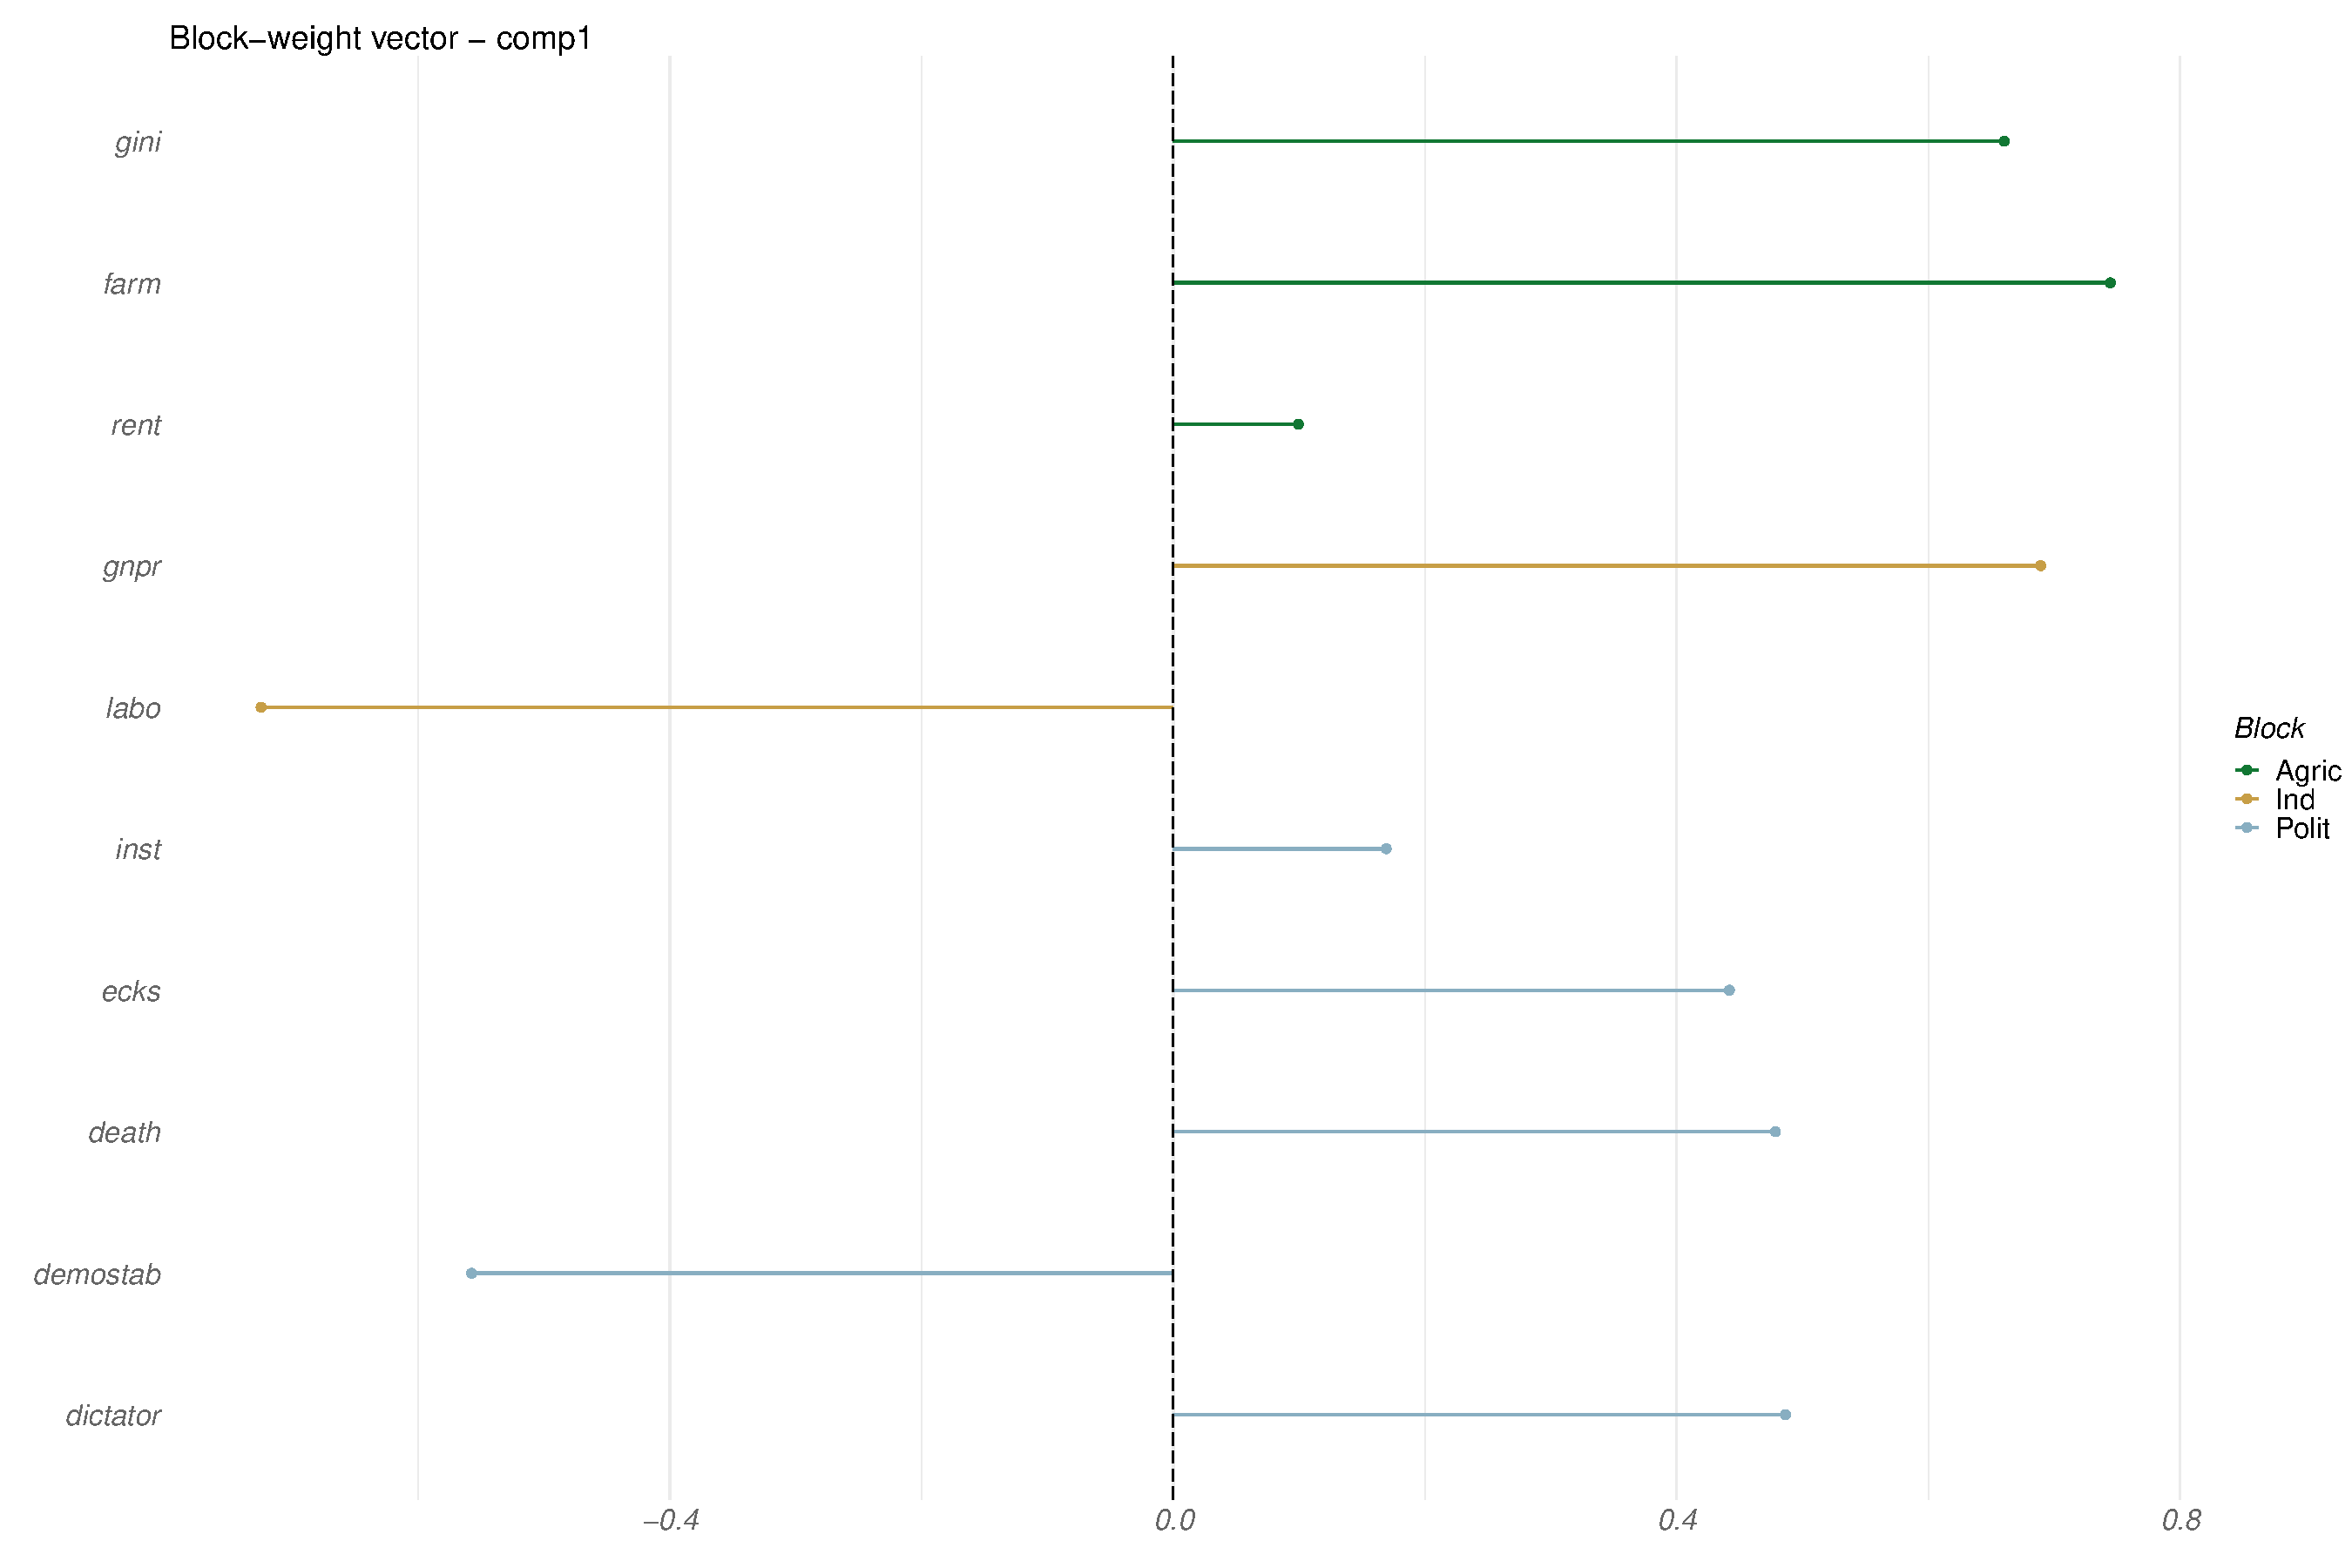
\includegraphics{RGCCA_vignette_files/figure-latex/unnamed-chunk-7-1} 

}

\caption[block weight vectors]{block weight vectors}\label{fig:unnamed-chunk-7}
\end{figure}
\end{CodeChunk}

\normalsize

As component-based method, the RGCCA package provides block components
as output of the \texttt{rgcca()} function in \texttt{fit\$Y} and
graphical representations, including factor plot
(\texttt{type\ =\ "sample"}), correlation circle
(\texttt{type\ =\ "cor\_circle"}) or biplot
(\texttt{type\ =\ "biplot"}). This graphical displays allows visualizing
the sources of variability within blocks, the relationships between
variables within and between blocks and the amount of correlation
between blocks. The graphical display of the countries obtained by
crossing \(\X_1 \ma a_1\) = Agricultural Inequality and \(\X_2 \ma a_2\)
= Industrial Development and marked with their political regime in 1960
is shown in below.

\footnotesize

\begin{CodeChunk}
\begin{CodeInput}
R> plot(fit, type = "sample",
+      block = 1:2, comp = 1,
+      resp = lab, repel = TRUE, cex = 1.3)
\end{CodeInput}
\begin{figure}

{\centering 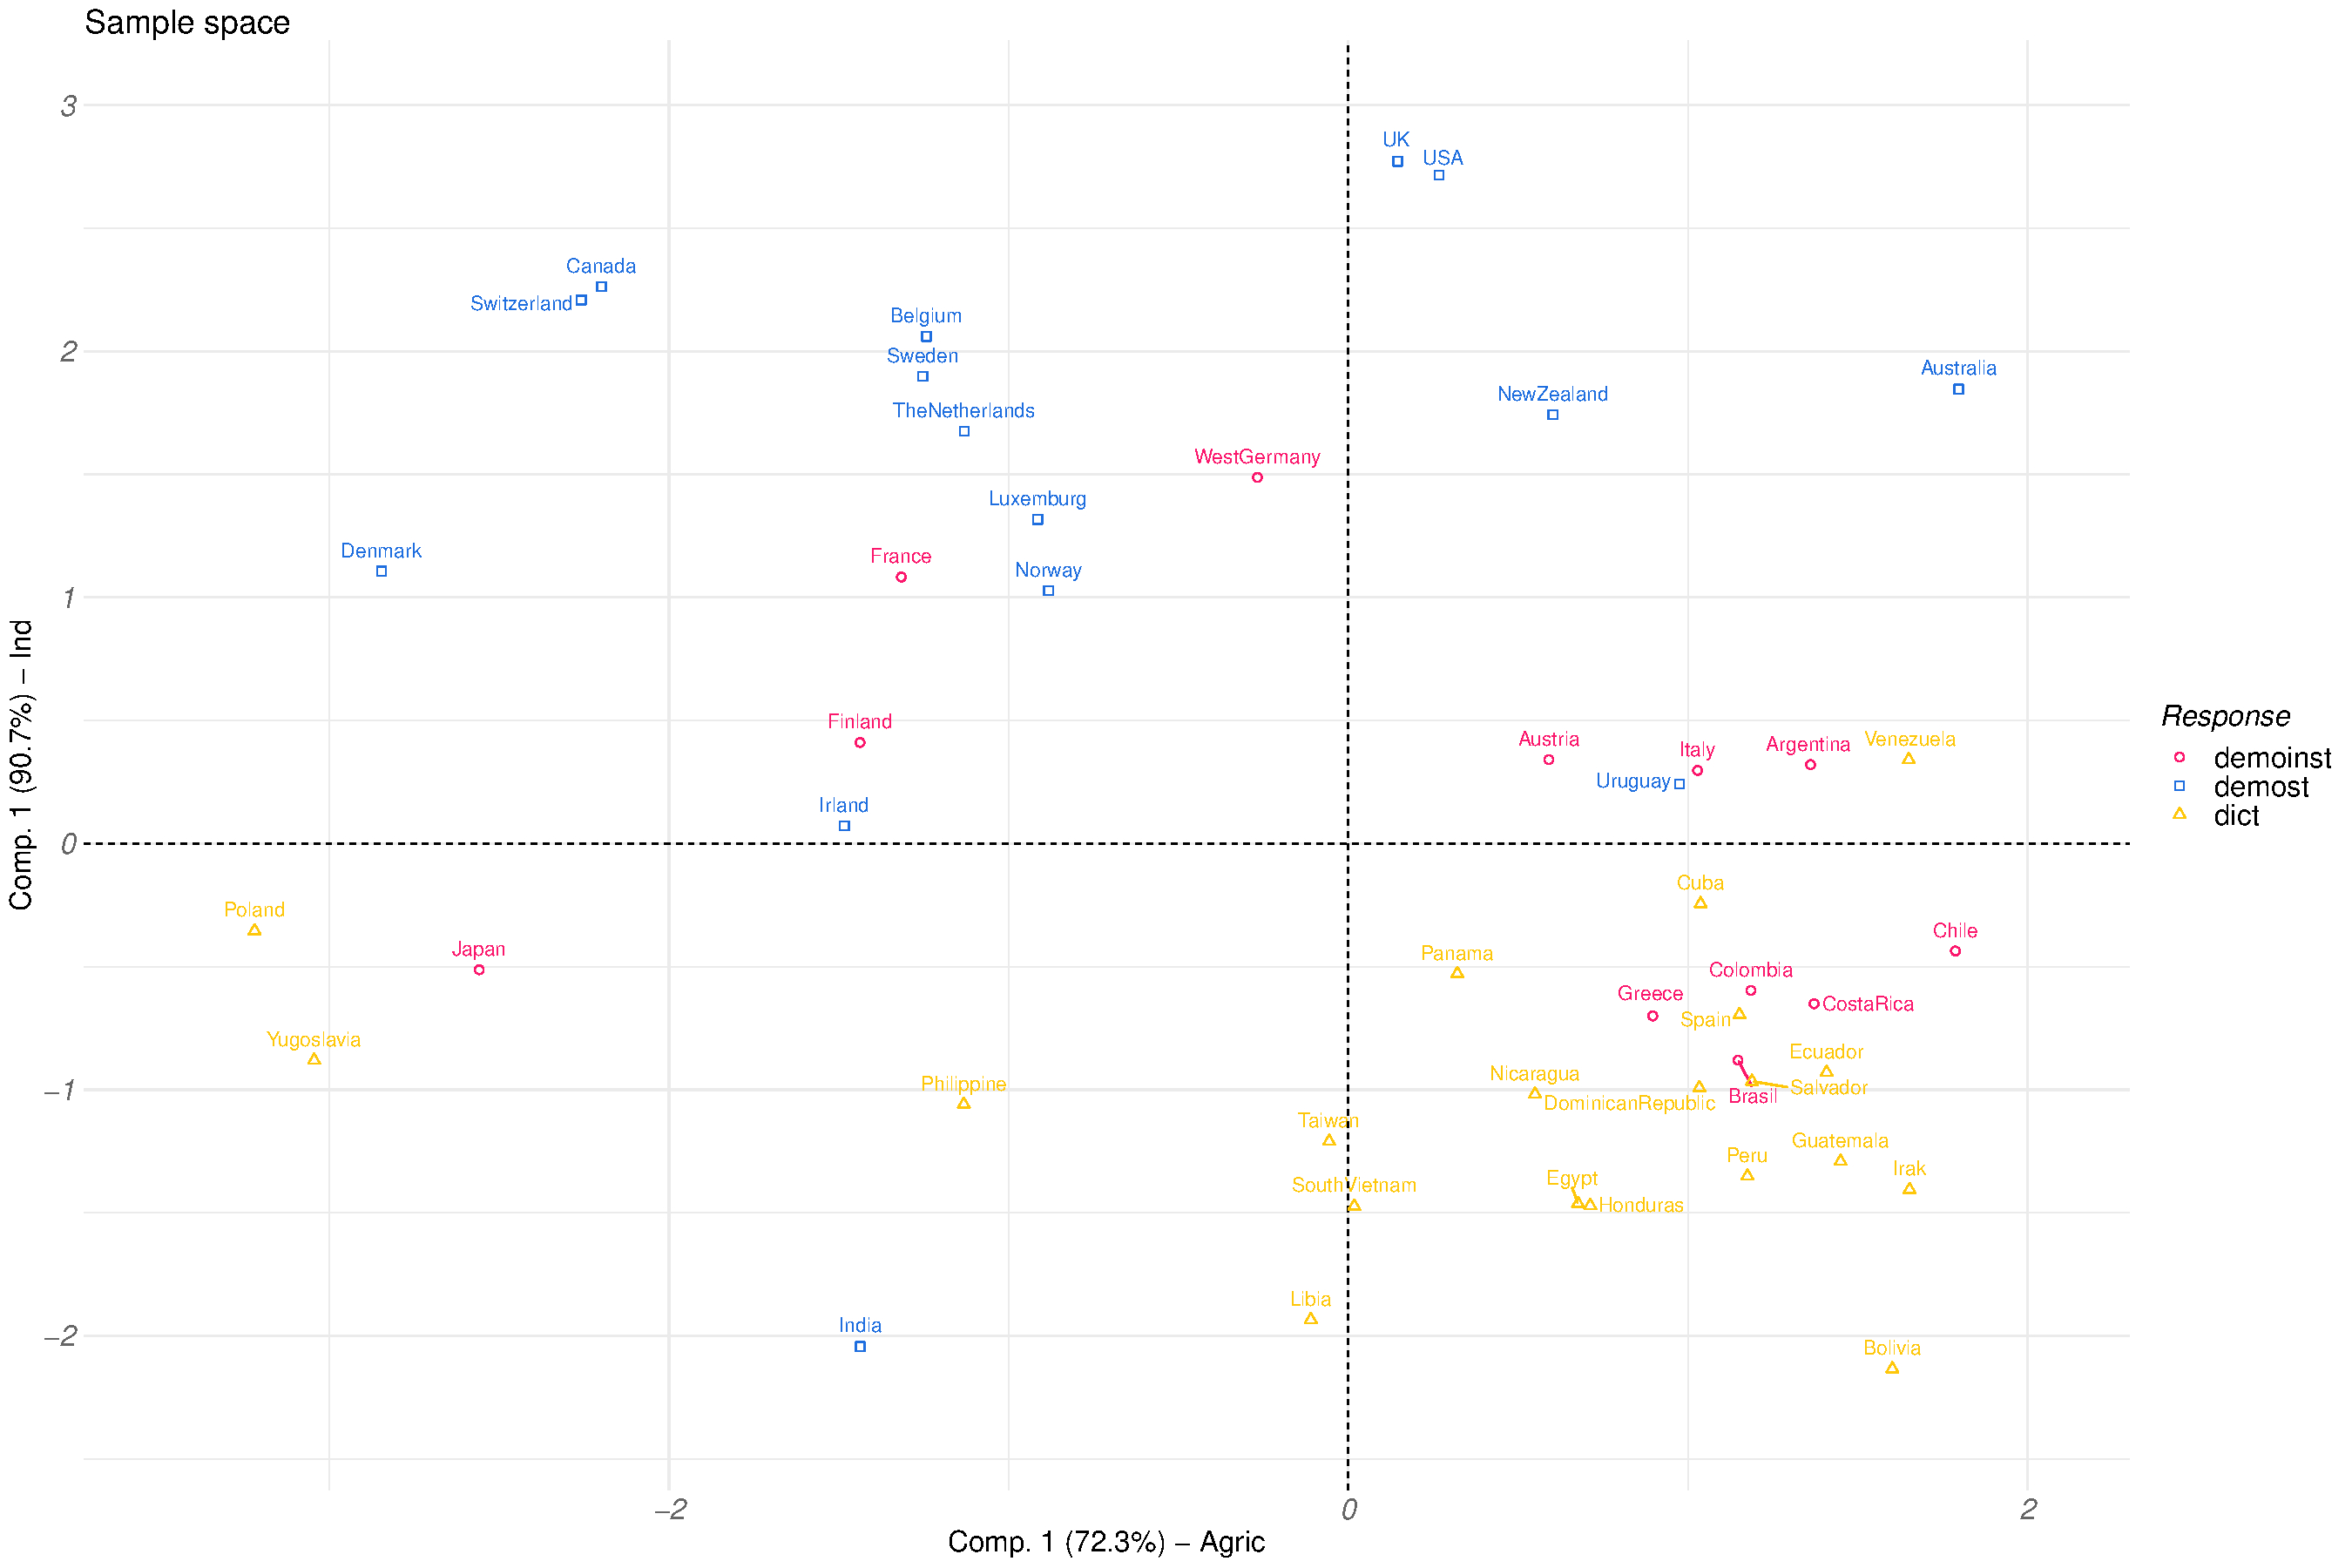
\includegraphics{RGCCA_vignette_files/figure-latex/unnamed-chunk-8-1} 

}

\caption[graphical display of the countries obtained by crossing y11 and y21 and labeled according to their political regime]{graphical display of the countries obtained by crossing y11 and y21 and labeled according to their political regime}\label{fig:unnamed-chunk-8}
\end{figure}
\end{CodeChunk}

\normalsize

Countries aggregate together when they share similarities. It may be
noted that the lower right quadrant concentrates on dictatorships. It is
difficult for a country to escape dictatorship when its industrial
development is below-average and its agricultural inequality is above
average. It is worth pointing out that some unstable democracies located
in this quadrant (or close to it) became dictatorships for a period of
time after 1960: Greece (1967-1974), Brazil (1964-1985), Chili
(1973-1990), and Argentina (1966-1973). The Average Variance Explained
(AVE) defined below is also reported in the axes of the Figure. The AVE
of block \(\mathbf{X}_j\) for a specific block component
\(\mathbf{y}_j\) is defined as:

\begin{equation}
\mathrm{AVE}(\X_j)=  \frac{1}{\Vert \X_j \Vert^2} \sum_{h=1}^{p_j} \text{var}(\mathbf{x}_{jh}) \times \text{cor}^2(\mathbf{x}_{jh},\mathbf{y}_j)
\end{equation}

AVE(\(\X_j\)) varies between 0 and 1 and reflects the proportion of
variance captured by \(\mathbf{y}_j\).

Additional indicators of model quality are also proposed:

\begin{itemize}
\tightlist
\item
  For all blocks:
\end{itemize}

\begin{equation}
\displaystyle \mathrm{AVE(outer model)} = \left( 1/\sum_j \Vert \X_j \Vert^2 \right) \sum_j \Vert \X_j \Vert^2 \mathrm{AVE}(\X_j)
\end{equation}

\begin{itemize}
\tightlist
\item
  For the inner model:
\end{itemize}

\begin{equation}
\displaystyle \mathrm{AVE(inner model)} = \left( 1/\sum_{j<k} c_{jk} \right) \sum_{j<k} c_{jk} \mathrm{cor}^2(\mathbf{y}_j , \mathbf{y}_k)
\end{equation}

These indicators of model quality are also available as output of the
\texttt{rgcca()} function in \texttt{fit\$AVE}. These AVEs can be
visualized using the generic \texttt{plot()} function.

\footnotesize

\begin{CodeChunk}
\begin{CodeInput}
R> plot(fit, type = "ave", cex = 1.3)
\end{CodeInput}
\begin{figure}[H]

{\centering 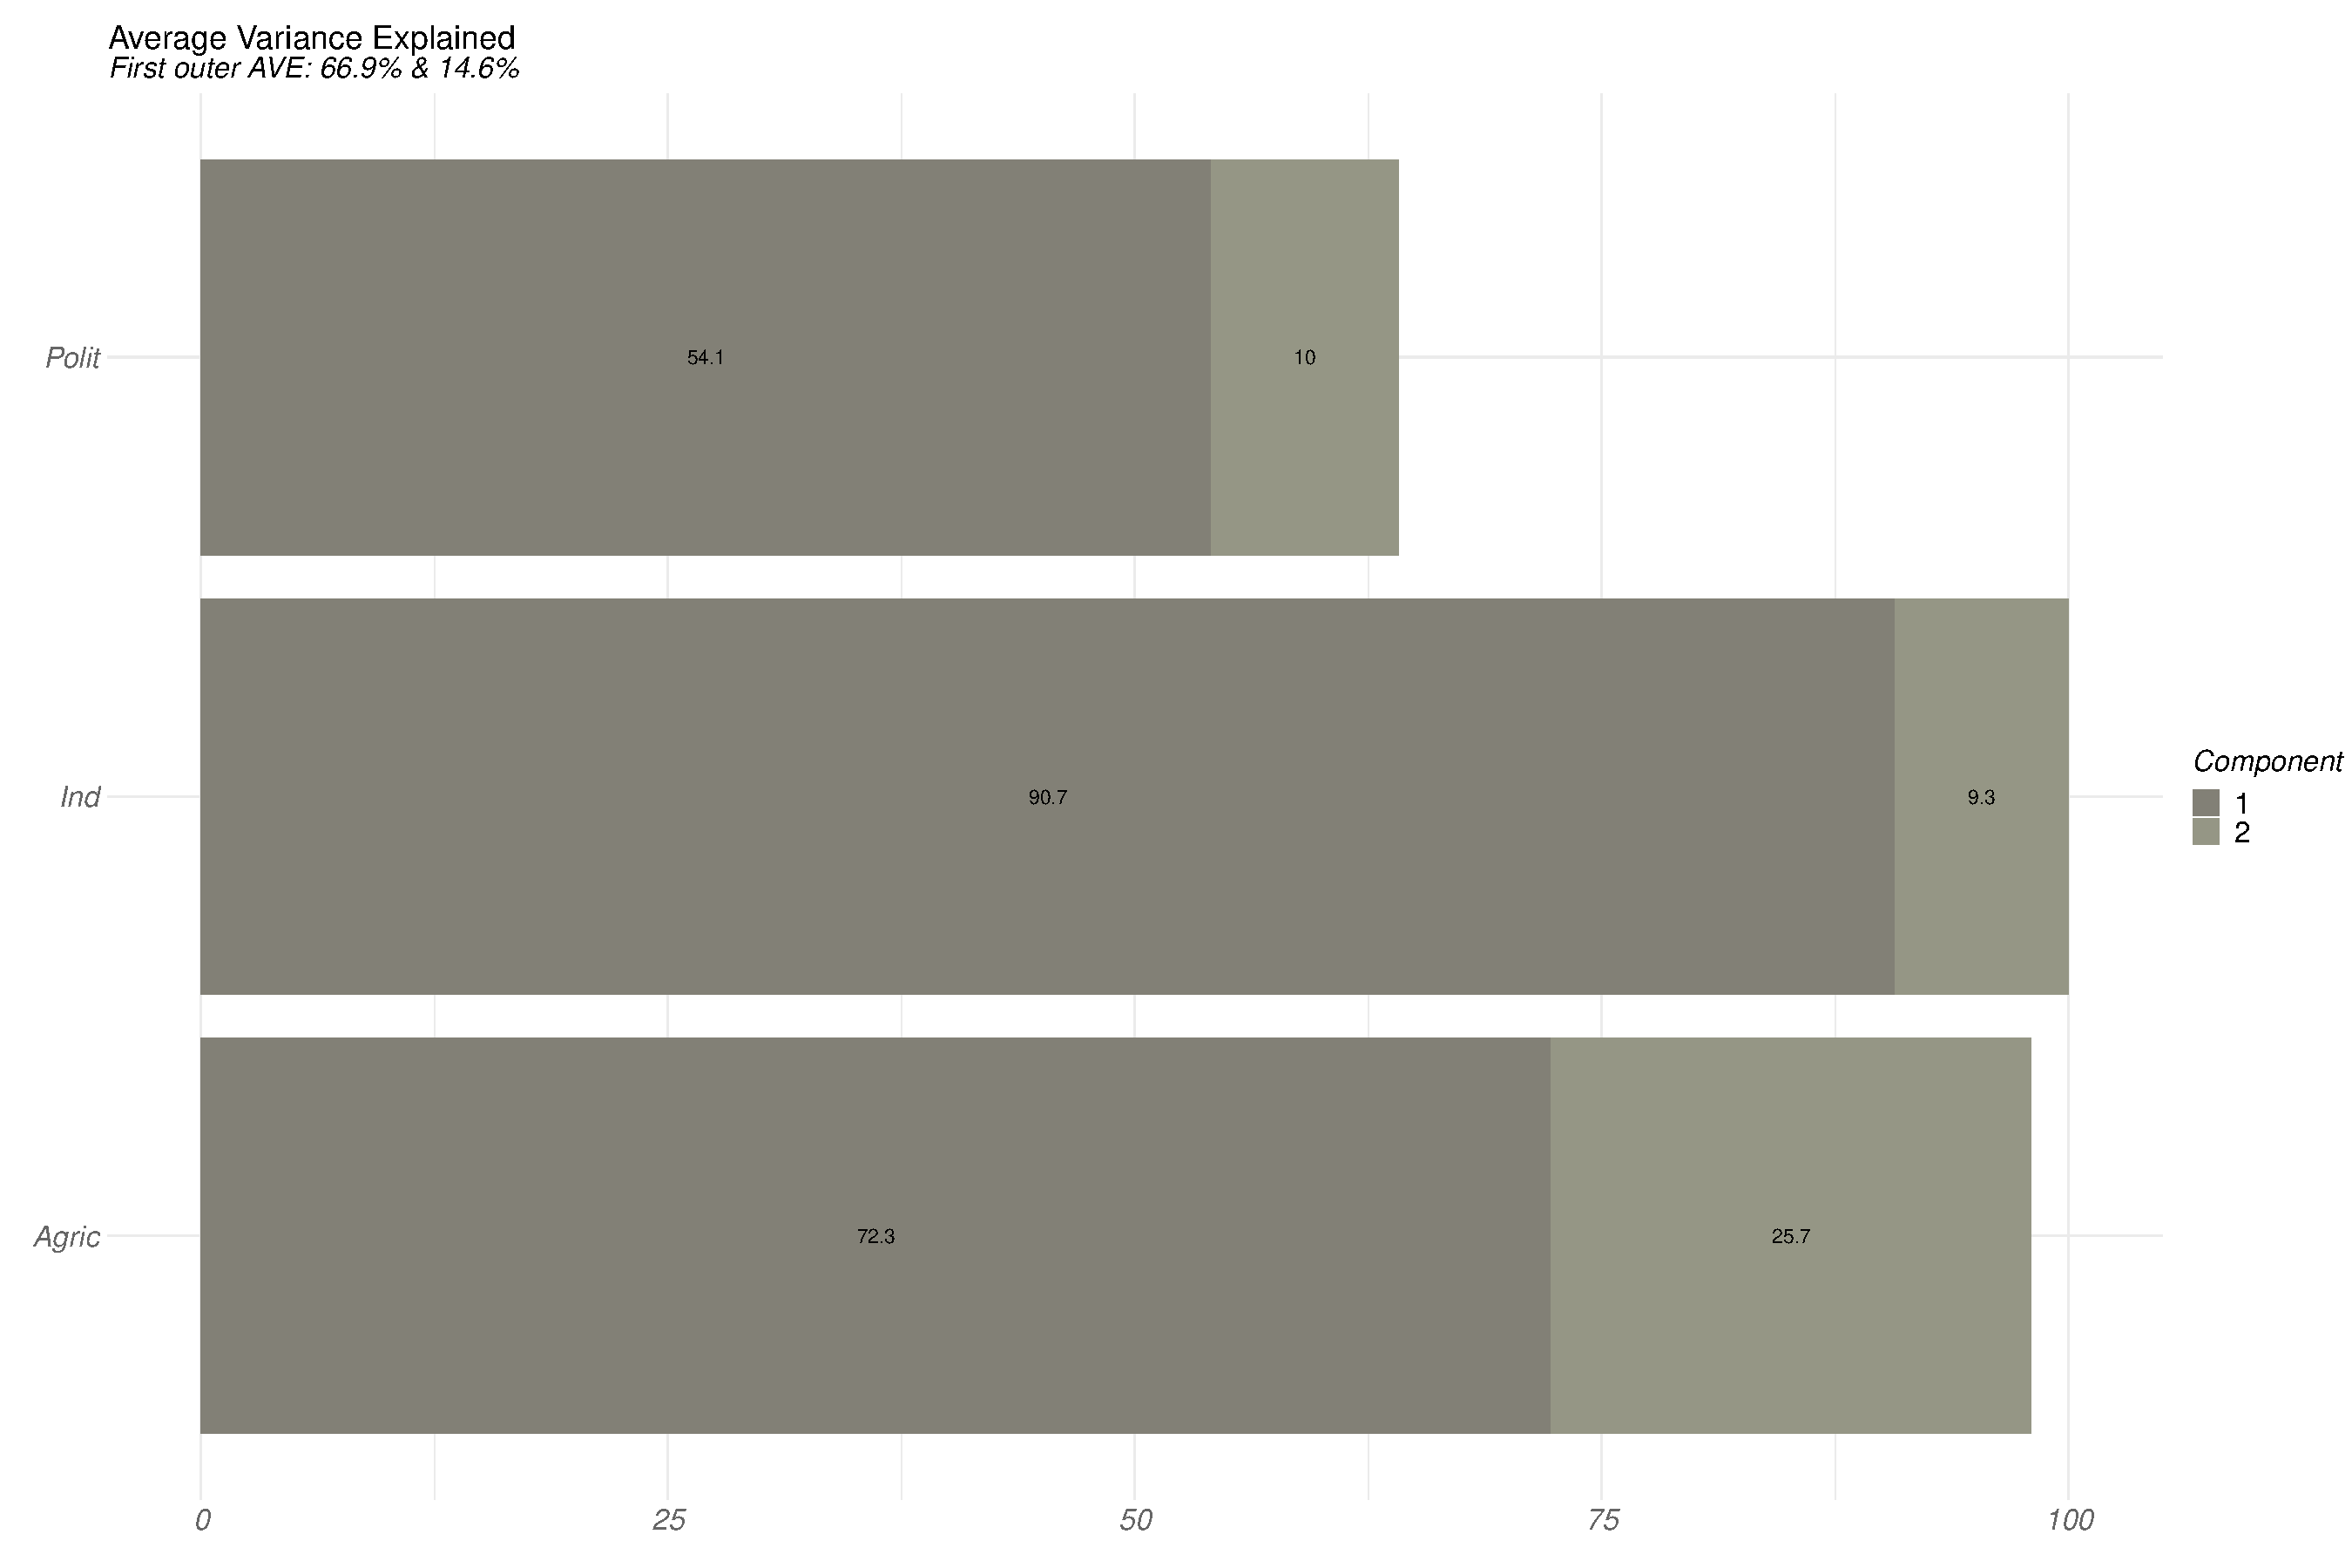
\includegraphics{RGCCA_vignette_files/figure-latex/unnamed-chunk-9-1} 

}

\caption[Average variance explained of the various blocks]{Average variance explained of the various blocks}\label{fig:unnamed-chunk-9}
\end{figure}
\end{CodeChunk}

\normalsize

The strength of the relations between each block component and each
variable can be visualized using correlation circle or biplot
representations.

\footnotesize

\begin{CodeChunk}
\begin{CodeInput}
R> plot(fit, type = "cor_circle", block = 1, comp = 1:2, display_blocks = 1:3)
\end{CodeInput}
\begin{figure}

{\centering 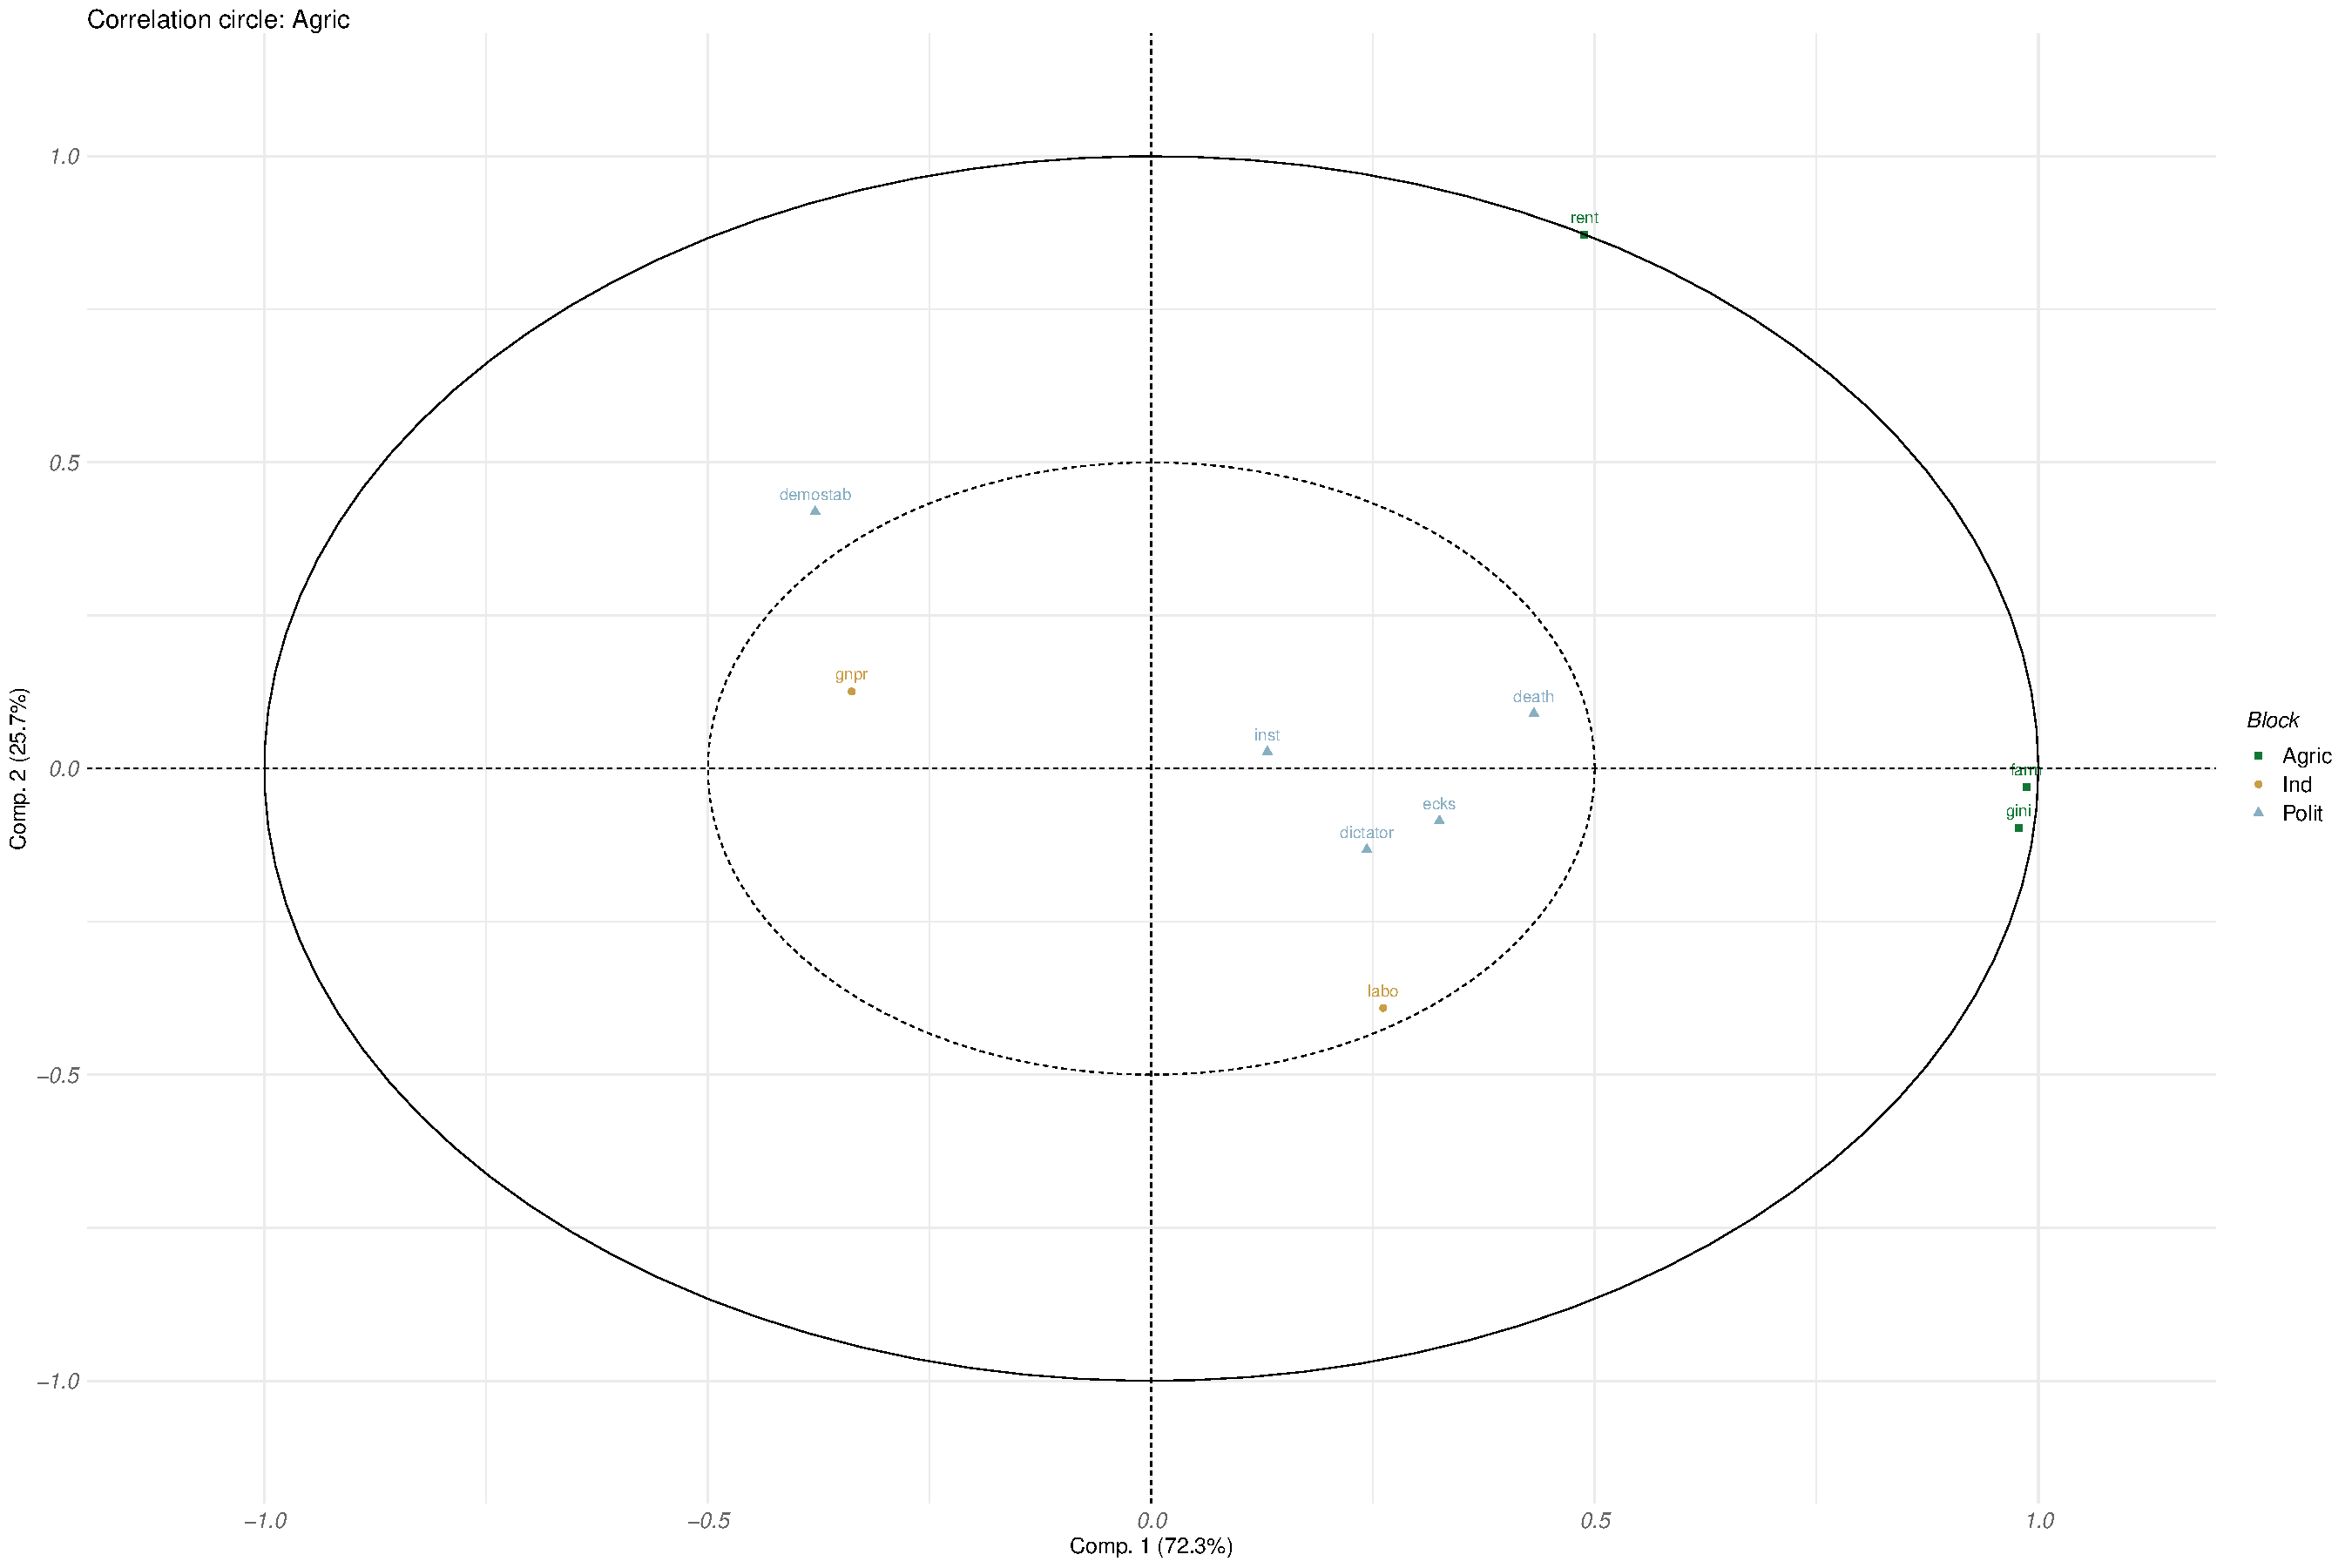
\includegraphics{RGCCA_vignette_files/figure-latex/unnamed-chunk-10-1} 

}

\caption[correlation circle associated with the two first components of Ariculture]{correlation circle associated with the two first components of Ariculture}\label{fig:unnamed-chunk-10}
\end{figure}
\end{CodeChunk}

\normalsize

By default all the variables are displayed on the correlation circle.
However, it is possible to choose the block(s) to display
(\texttt{display\_blocks})in the correlation\_circle.

\footnotesize

\begin{CodeChunk}
\begin{CodeInput}
R> plot(fit, type = "biplot", block = 1, 
+      comp = 1:2, repel = TRUE, 
+      resp = lab, 
+      show_arrow = TRUE)
\end{CodeInput}
\begin{figure}

{\centering 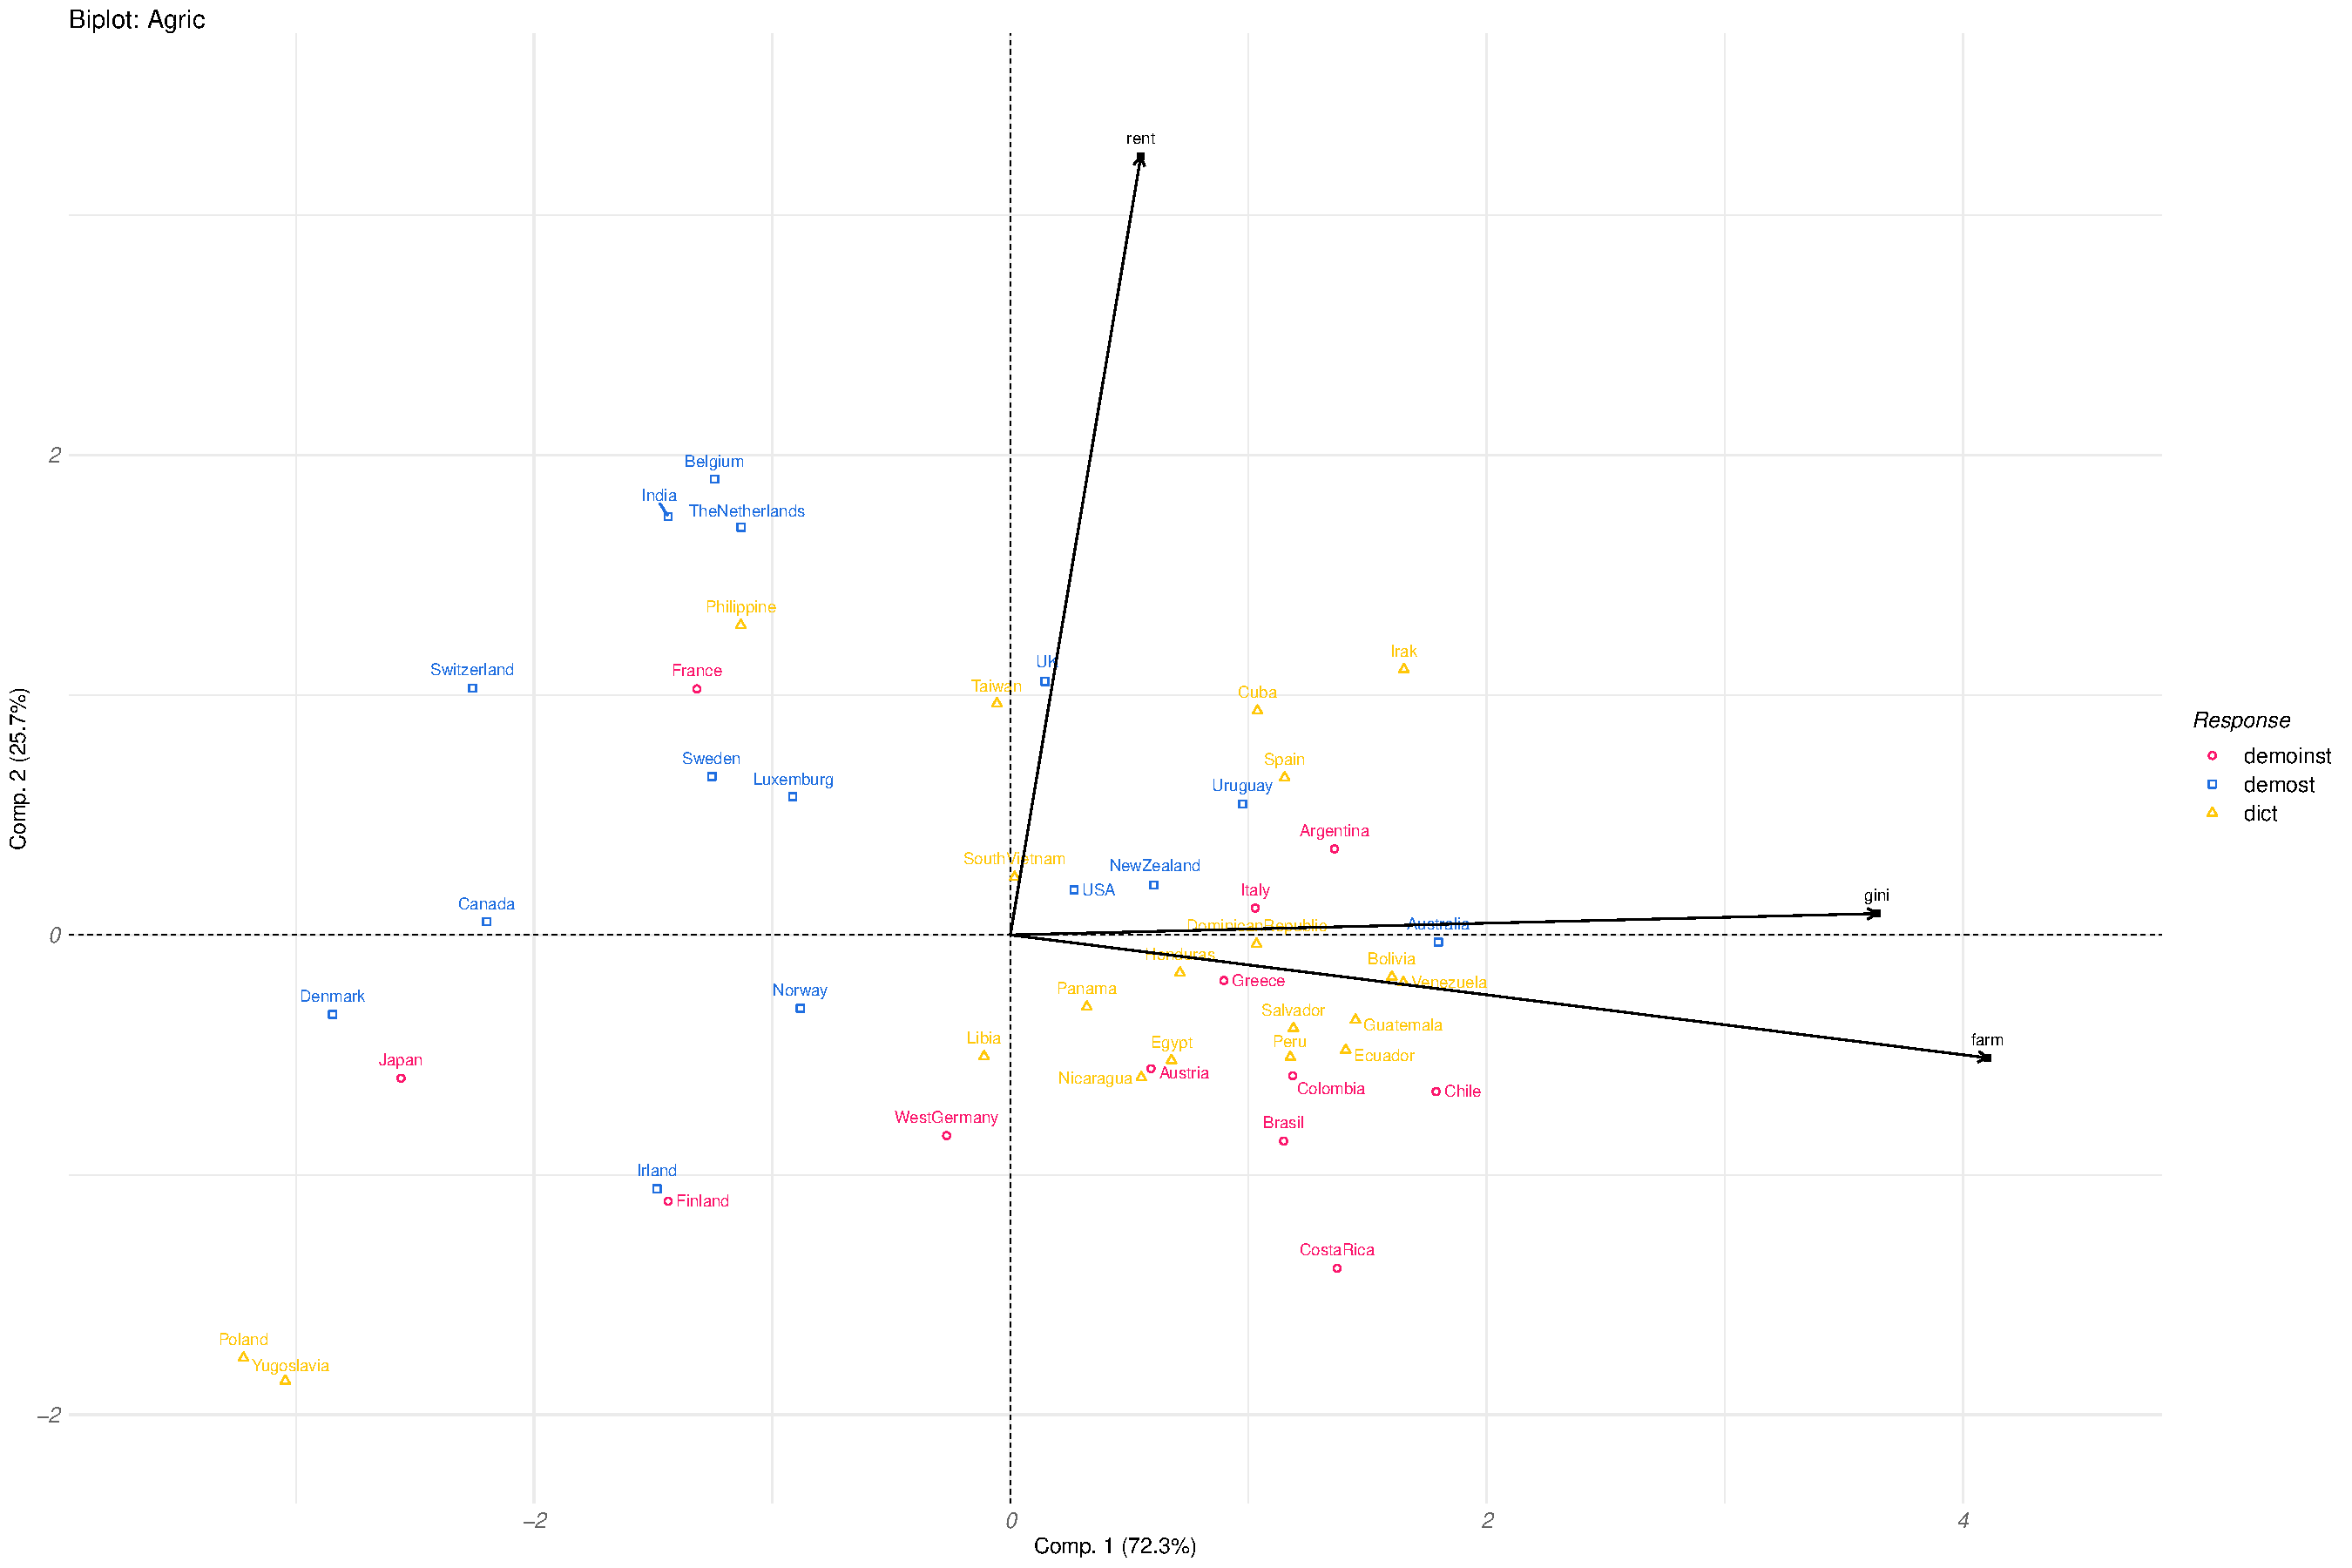
\includegraphics{RGCCA_vignette_files/figure-latex/unnamed-chunk-11-1} 

}

\caption[biplot associated with the two first components of Ariculture]{biplot associated with the two first components of Ariculture}\label{fig:unnamed-chunk-11}
\end{figure}
\end{CodeChunk}

\normalsize

As we will see in the next section, when the superblock option is
considered (\texttt{superblock\ =\ TRUE} or \texttt{method} set to a
method that induces the use of superblock) global components can be
derived. The space spanned by the global components can be viewed as a
consensus space that integrated all the modalities and facilitates the
visualization of the results and their interpretation.

\textbf{Assessment of the reliability of parameter estimates.} It is
possible to use a bootstrap resampling method to assess the reliability
of parameter estimates (block-weight/loading vectors) obtained using
RGCCA. \(B=\)\texttt{n\_boot} bootstrap samples of the same size as the
original data is repeatedly sampled with replacement from the original
data. RGCCA is then applied to each bootstrap sample to obtain the RGCCA
estimates. We calculate the standard deviation of the estimates across
the bootstrap samples, from which we derived, bootstrap confidence
intervals, t-ratio (defined as the ratio of the parameter estimate to
its bootstrap estimate of the standard deviation) and p-value (the
p-value is computed by assuming that the ratio of the parameter estimate
to its standard deviation follows the standardized normal distribution)
to indicate how reliably parameters were estimated. Since several
p-values are constructed simultaneously, FDR correction can be applied
for controlling the False Discovery Rate. This function is available
using the \texttt{rgcca\_bootstrap()} function of the RGCCA package.

\footnotesize

\begin{CodeChunk}
\begin{CodeInput}
R> boot_out = rgcca_bootstrap(fit, n_boot = 500, n_cores = 1)
\end{CodeInput}
\end{CodeChunk}

\normalsize

The bootstrap results are detailed using the \texttt{print()} function.

\footnotesize

\begin{CodeChunk}
\begin{CodeInput}
R> print(boot_out, block = 1:3, ncomp = 1)
\end{CodeInput}
\begin{CodeOutput}
Call: method='rgcca', superblock=FALSE, scale=TRUE, scale_block=FALSE, init='svd',
bias=TRUE, tol=1e-08, NA_method='nipals', ncomp=c(2,2,2), response=NULL,
comp_orth=TRUE 
There are J = 3 blocks.
The design matrix is:
      Agric Ind Polit
Agric     0   0     1
Ind       0   0     1
Polit     1   1     0

The factorial scheme is used.

Extracted statistics from 500 bootstrap samples.
Block-weight vectors for component 1: 
         estimate    mean     sd lower_bound upper_bound bootstrap_ratio
gini       0.6602  0.6347 0.0730      0.4575       0.734           9.050
farm       0.7445  0.7244 0.0928      0.6230       0.838           8.025
rent       0.0994  0.0788 0.2289     -0.4452       0.441           0.434
gnpr       0.6891  0.6885 0.0292      0.6236       0.740          23.610
labo      -0.7247 -0.7241 0.0271     -0.7817      -0.673         -26.768
inst       0.1692  0.1666 0.1119     -0.0655       0.364           1.512
ecks       0.4418  0.4347 0.0601      0.3046       0.532           7.356
death      0.4784  0.4708 0.0485      0.3771       0.563           9.857
demostab  -0.5574 -0.5518 0.0516     -0.6515      -0.452         -10.801
dictator   0.4864  0.4830 0.0521      0.3743       0.585           9.343
            pval adjust.pval
gini     0.00000     0.00000
farm     0.00402     0.00618
rent     0.44509     0.52363
gnpr     0.00000     0.00000
labo     0.00000     0.00000
inst     0.07066     0.10095
ecks     0.00000     0.00000
death    0.00000     0.00000
demostab 0.00000     0.00000
dictator 0.00000     0.00000
\end{CodeOutput}
\end{CodeChunk}

\normalsize

and displayed using the \texttt{plot()}function.

\footnotesize

\begin{CodeChunk}
\begin{CodeInput}
R> plot(boot_out, type = "weight", 
+      block = 1:3, comp = 1, 
+      display_order = FALSE, cex = 1.3,
+      show_stars = TRUE)
\end{CodeInput}


\begin{center}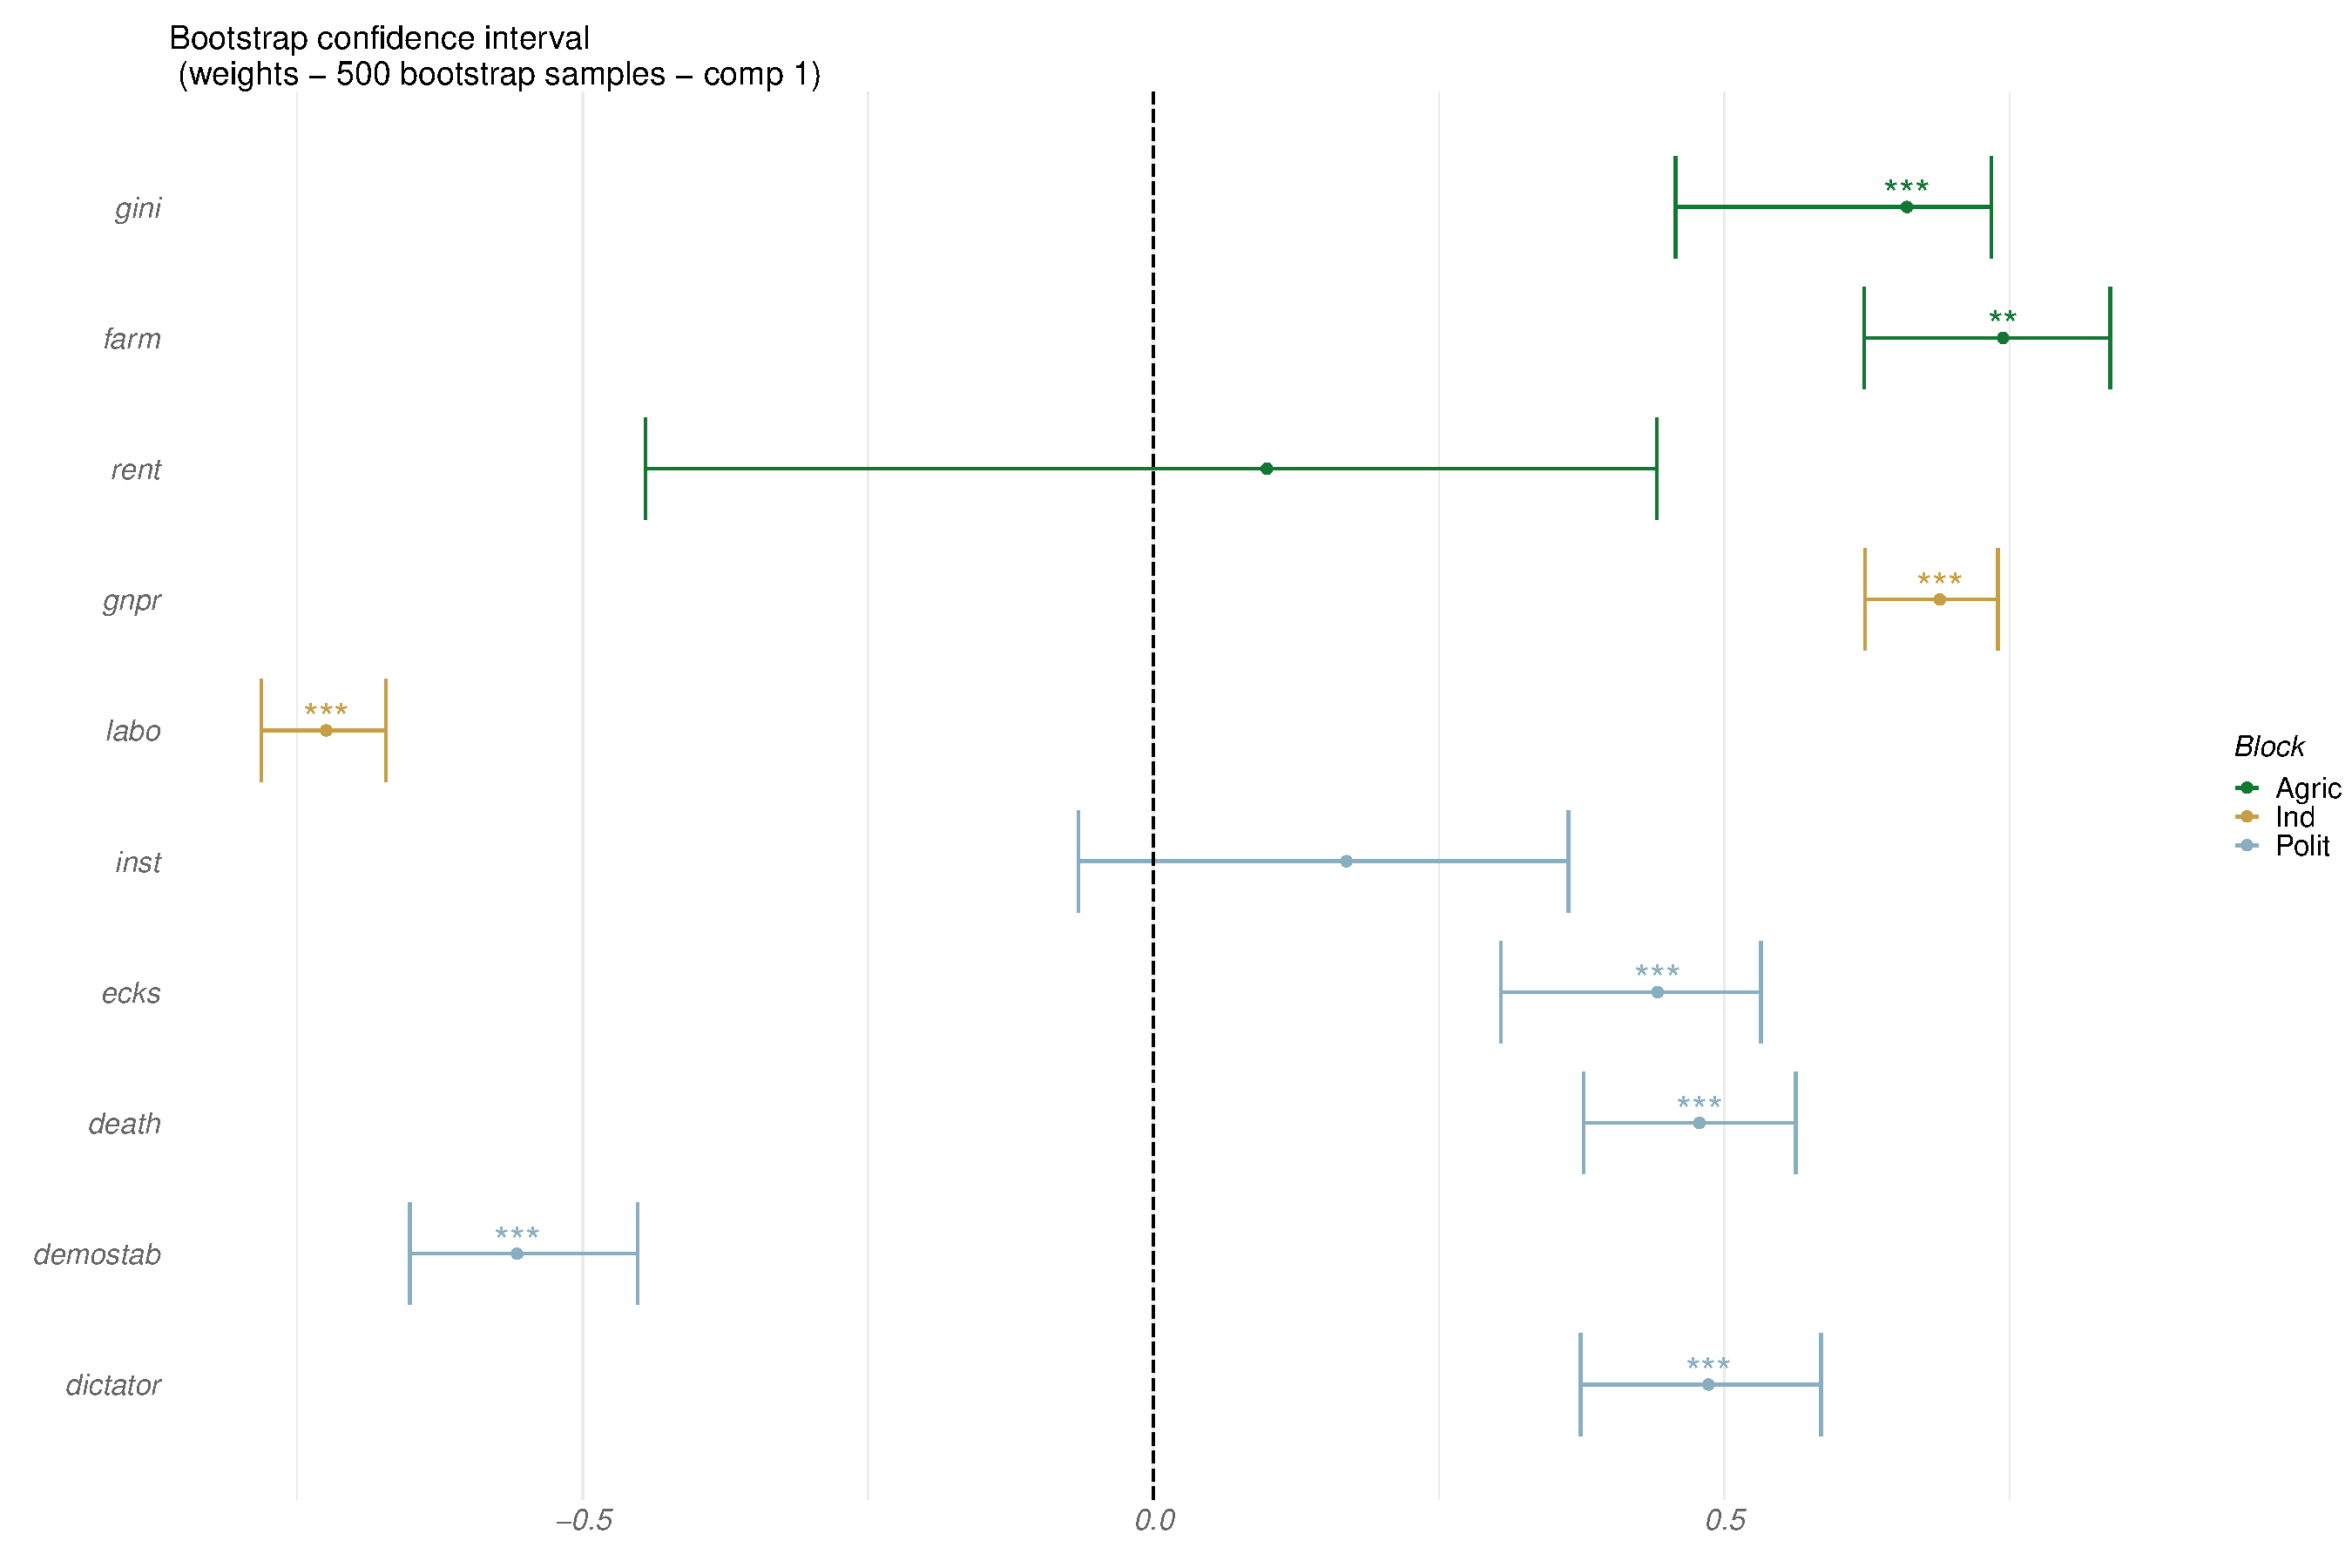
\includegraphics{RGCCA_vignette_files/figure-latex/unnamed-chunk-14-1} \end{center}

\end{CodeChunk}

\normalsize

Each weight is shown along with its associated bootstrap confidence
interval and stars (\texttt{show\_stars\ =\ TRUE}) reflecting the
p-value of assigning a strictly positive or negative weight to this
variable.

\hypertarget{rgcca-with-superblock}{%
\subsection{RGCCA with superblock}\label{rgcca-with-superblock}}

In this section, we consider Multiple Co-Inertia Analysis
\citep{Chessel1996} (MCOA, also called MCIA in \citep{Cantini2021}) with
\(2\) components per block.

See \texttt{available\_methods()} for a list of pre-specified multiblock
component methods.

\footnotesize

\begin{CodeChunk}
\begin{CodeInput}
R> fit.mcoa = rgcca(blocks=A, method = "mcoa", ncomp = 2)
\end{CodeInput}
\end{CodeChunk}

\normalsize

the \texttt{print()} function allows summarizing the RGCCA analysis.

\footnotesize

\begin{CodeChunk}
\begin{CodeInput}
R> print(fit.mcoa)
\end{CodeInput}
\begin{CodeOutput}
Call: method='mcoa', superblock=TRUE, scale=TRUE, scale_block='inertia', init='svd',
bias=TRUE, tol=1e-08, NA_method='nipals', ncomp=c(2,2,2,2), response=NULL,
comp_orth=FALSE 
There are J = 4 blocks.
The design matrix is:
           Agric Ind Polit superblock
Agric          0   0     0          1
Ind            0   0     0          1
Polit          0   0     0          1
superblock     1   1     1          0

The factorial scheme is used.
Sum_{j,k} c_jk g(cov(X_j a_j, X_k a_k) = 3.578 

The regularization parameter used for Agric is: 1
The regularization parameter used for Ind is: 1
The regularization parameter used for Polit is: 1
The regularization parameter used for superblock is: 0
\end{CodeOutput}
\end{CodeChunk}

\normalsize

Interestingly, this output reports the arguments that has been
implicitly specified to reach MCOA.

It is possible to display specific output as previously using the
generic \texttt{plot()} function by specifying the argument
\texttt{type} accordingly. MCOA enables the individuals to be
represented in the space spanned by the two first global components. The
biplot representation associated with this consensus space is given
below.

\footnotesize

\begin{CodeChunk}
\begin{CodeInput}
R> plot(fit.mcoa, type = "biplot", 
+      block = 4, comp = 1:2, 
+      response = lab, 
+      repel = TRUE, cex = 1.3)
\end{CodeInput}
\begin{figure}

{\centering 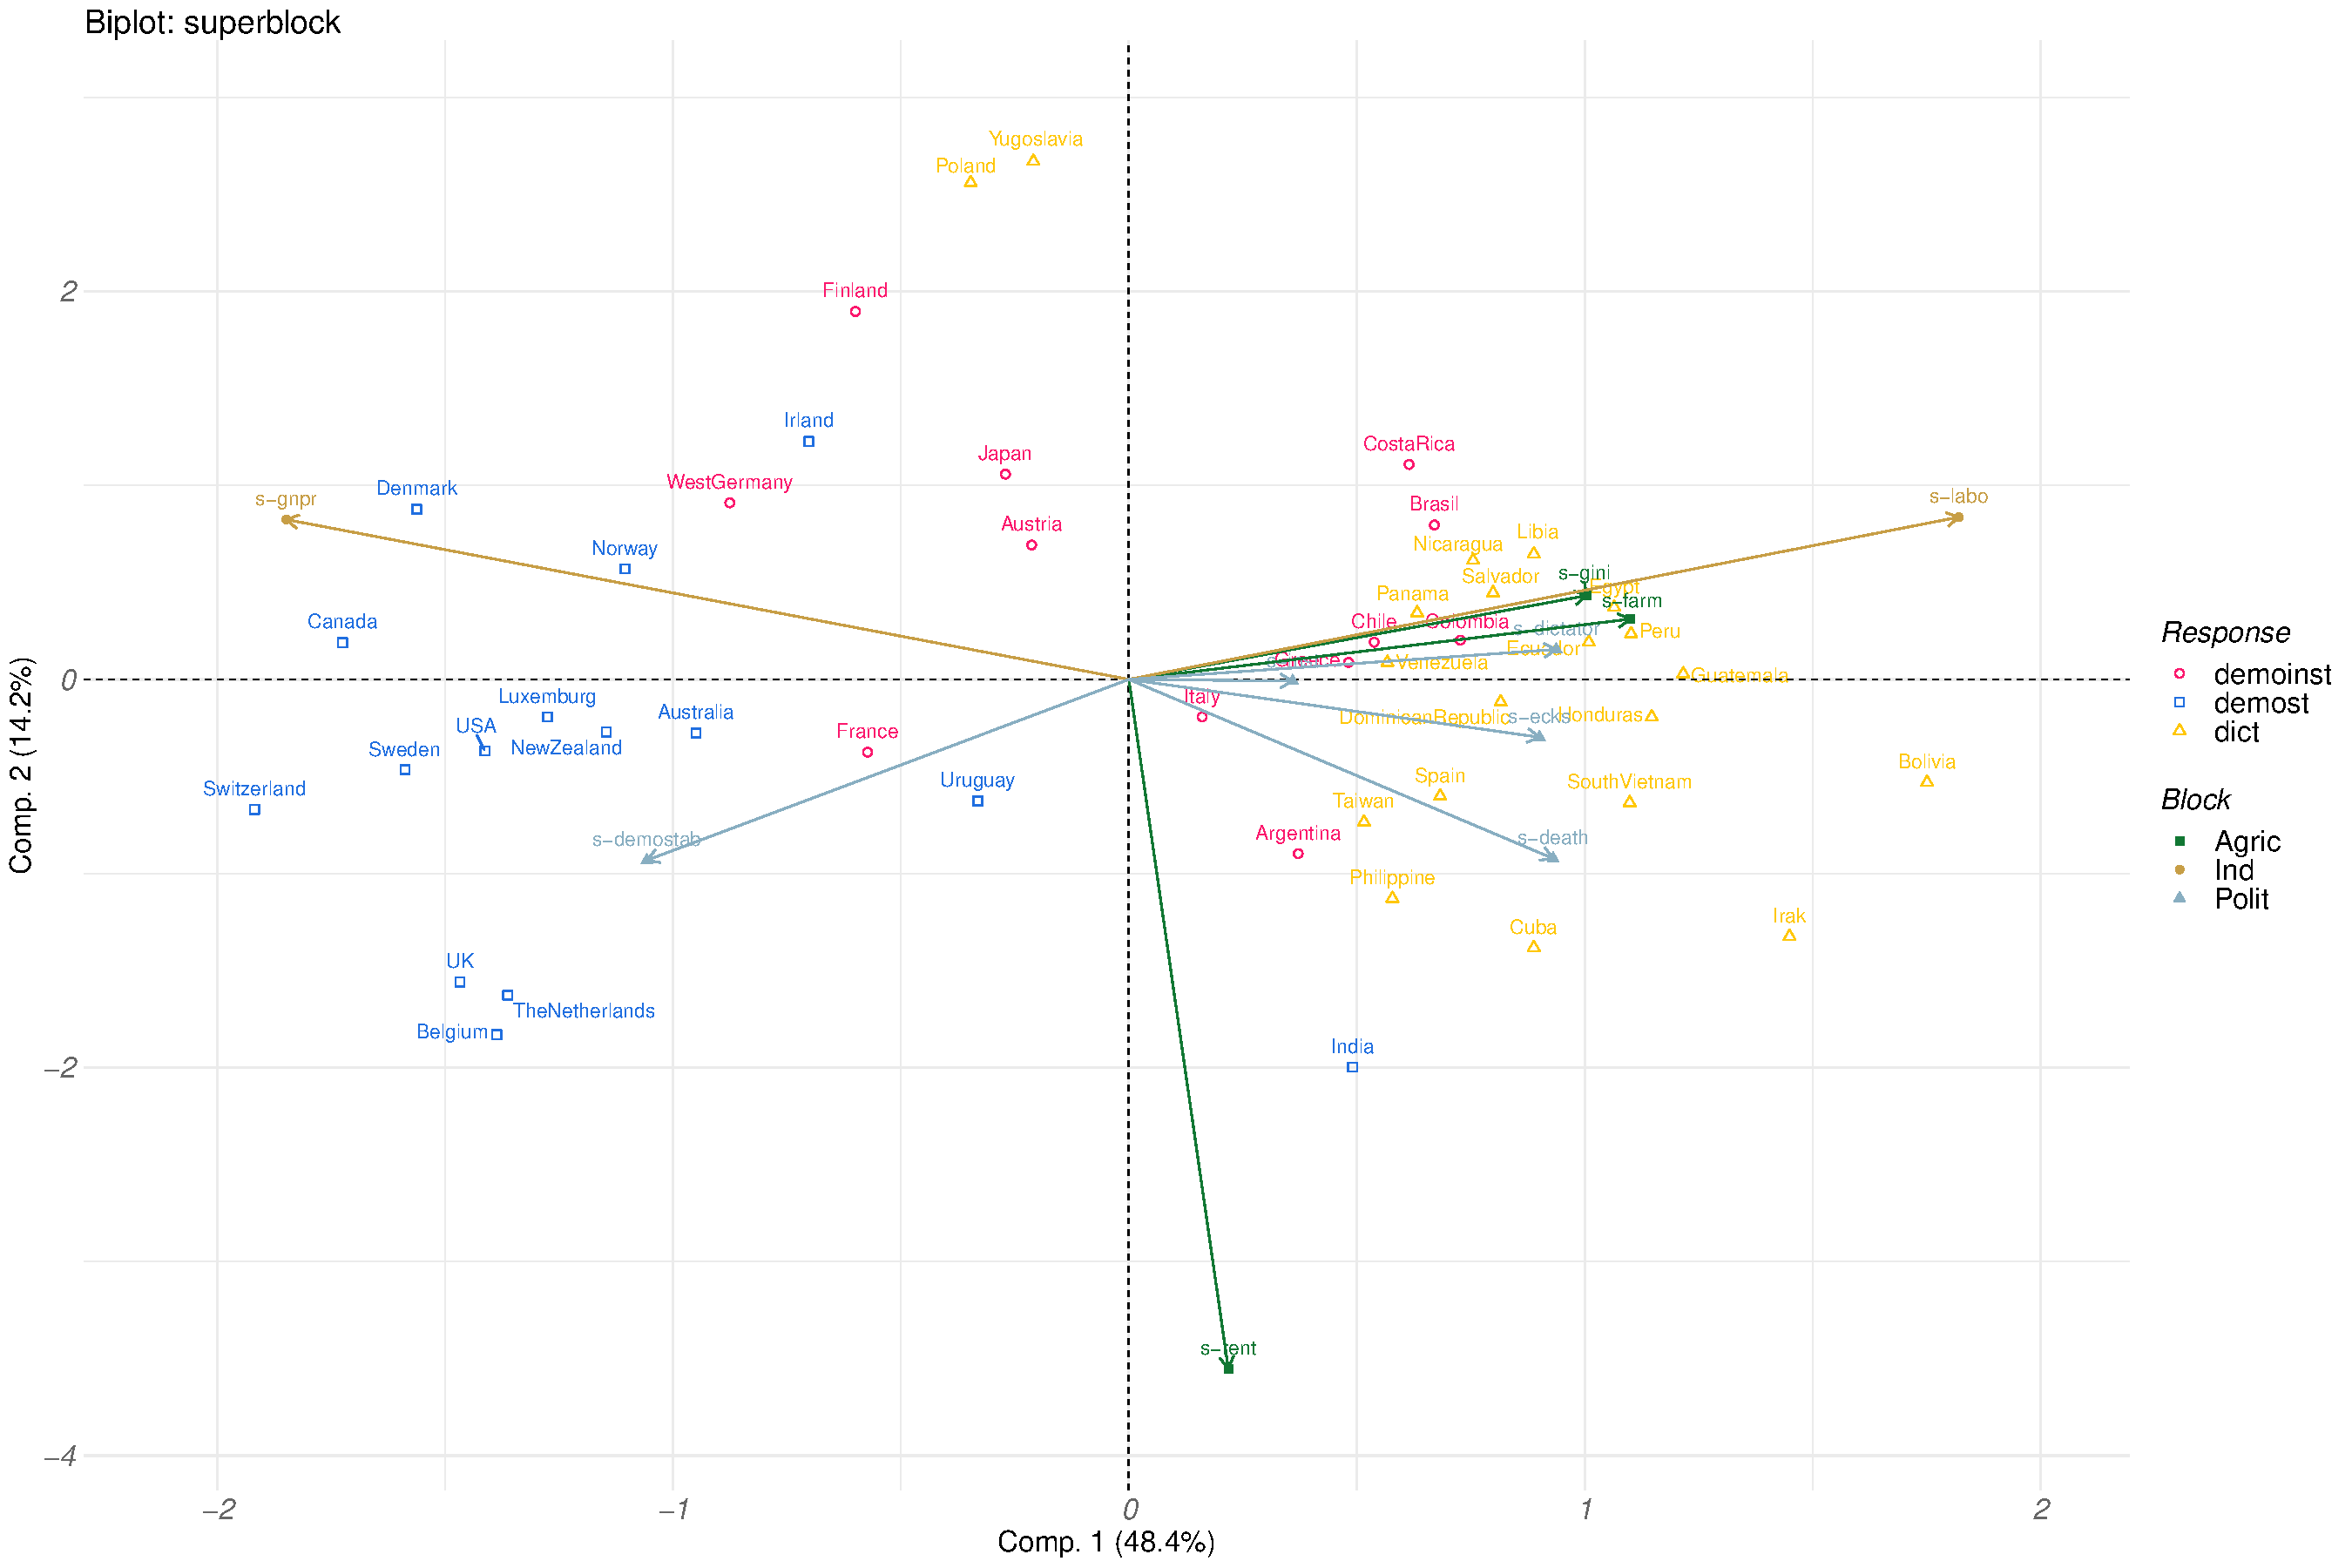
\includegraphics{RGCCA_vignette_files/figure-latex/unnamed-chunk-17-1} 

}

\caption[A biplot graphical display of the countries obtained by crossing the two first components of the superblock]{A biplot graphical display of the countries obtained by crossing the two first components of the superblock. Individuals are labeled according to their political regime and variables according to their block membership.}\label{fig:unnamed-chunk-17}
\end{figure}
\end{CodeChunk}

\normalsize

As previously, this model can be easily bootstrapped using the
\texttt{rgcca\_bootstrap()} function and the bootstrap confidence
intervals are still available using the \texttt{print()/plot()}
functions.

\hypertarget{choice-of-the-shrinkage-parameters}{%
\subsection{Choice of the shrinkage
parameters}\label{choice-of-the-shrinkage-parameters}}

Three fully automatic strategies are proposed to select the optimal
shrinkage parameters:

\textbf{The Schafer and Strimmer analytical formula.} For each block
\(j\), an ``optimal'' shrinkage parameter \(\tau_j\) can be obtained
using the Schafer and Strimmer analytical formula \citep{Schafer2005} by
setting the \texttt{tau} argument of the \texttt{rgcca()} function to
\texttt{"optimal"}.

\footnotesize

\begin{CodeChunk}
\begin{CodeInput}
R> fit = rgcca(blocks = A, connection=C, response=3,
+             tau = "optimal", scheme = "factorial")
\end{CodeInput}
\end{CodeChunk}

\normalsize

The optimal shrinkage parameters are given by:

\footnotesize

\begin{CodeChunk}
\begin{CodeInput}
R> fit$call$tau
\end{CodeInput}
\begin{CodeOutput}
[1] 0.08853216 0.02703256 0.08422566
\end{CodeOutput}
\end{CodeChunk}

\normalsize

This automatic estimation of the shrinkage parameters allows one to come
closer to the correlation criterion, even in the case of high
multicollinearity or when the number of individuals is smaller than the
number of variables.

As previously, all the fitted RGCCA object can be visualized/bootstraped
using the \texttt{print}, \texttt{plot()} and
\texttt{rgcca\_bootstrap()} functions.

\textbf{Permutation strategy.} A permutation based strategy very similar
to the one proposed in \citep{Witten2009a} has been also integrated
within the RGCCA package through the \texttt{rgcca\_permutation()}
function. This function is used to select automatically the
regularization parameters for R/SGCCA.

For each set of regularization parameters (generally this will be a
\(J\)-dimensional vector), repeat the following \texttt{n\_perm} times,
for (\texttt{n\_perm} large):

\begin{enumerate}
\item [\label{p1}] The rows of $\mathbf X_1, \ldots, \mathbf X_J$ are
randomly permuted to obtained permuted data sets $\mathbf X_1^*, \ldots, \mathbf X_J^*$.

\item [\label{p2}] S/RGCCA is run on the permuted data set
$\mathbf X_1^*, \ldots, \mathbf X_J^*$ and we record the value of the 
objective function, denoted $t^*$.

\item [\label{p3}]  S/RGCCA is run on the original data 
$\mathbf X_1, \ldots, \mathbf X_J$ and we record the value of the objective 
function, denoted $t$.

\item [\label{p4}]  The resulting p-value is given by the fraction of permuted
$t*$ that exceed the real $t$t obtained from the non-permuted blocks.
\end{enumerate}

Then choose the set of tuning parameters that yields the smallest value
in step (\ref{p4}). This procedure is available though the
\texttt{rgcca\_permutation()} function.

\footnotesize

\begin{CodeChunk}
\begin{CodeInput}
R> set.seed(123)
R> perm_out = rgcca_permutation(blocks = A, connection=C, 
+                              par_type = "tau",
+                              par_value = c(.51, .13, 0),
+                              par_length = 10,
+                              n_cores = 1,
+                              n_perms = 10)
\end{CodeInput}
\end{CodeChunk}

\normalsize

By default, the \texttt{rgcca\_permutation()} function takes 10 sets of
tuning parameters between min values (0 for RGCCA and \(1/sqrt(ncol)\)
for SGCCA) and 1. Results of the permutation procedure are
summarized/displayed using the generic \texttt{print()/plot()} function

\footnotesize

\begin{CodeChunk}
\begin{CodeInput}
R> print(perm_out)
\end{CodeInput}
\begin{CodeOutput}
Call: method='rgcca', superblock=FALSE, scale=TRUE, scale_block=TRUE, init='svd',
bias=TRUE, tol=1e-08, NA_method='nipals', ncomp=c(1,1,1), response=NULL,
comp_orth=TRUE 
There are J = 3 blocks.
The design matrix is:
      Agric Ind Polit
Agric     0   0     1
Ind       0   0     1
Polit     1   1     0

The factorial scheme is used.

Tuning parameters (tau) used: 
   Agric   Ind Polit
1  0.510 0.130     0
2  0.453 0.116     0
3  0.397 0.101     0
4  0.340 0.087     0
5  0.283 0.072     0
6  0.227 0.058     0
7  0.170 0.043     0
8  0.113 0.029     0
9  0.057 0.014     0
10 0.000 0.000     0

   Tuning parameters Criterion Permuted criterion    sd zstat p-value
1              Set 1      1.52              0.392 0.165  6.87       0
2              Set 2      1.54              0.400 0.168  6.76       0
3              Set 3      1.55              0.409 0.172  6.63       0
4              Set 4      1.57              0.420 0.176  6.50       0
5              Set 5      1.58              0.433 0.181  6.36       0
6              Set 6      1.61              0.448 0.187  6.20       0
7              Set 7      1.63              0.467 0.194  6.02       0
8              Set 8      1.67              0.493 0.203  5.82       0
9              Set 9      1.73              0.531 0.214  5.61       0
10            Set 10      1.93              0.665 0.230  5.52       0
The best combination is: Set 1 for a z score of 6.87 and a p-value of 0.
\end{CodeOutput}
\end{CodeChunk}

\normalsize

and displayed using the \texttt{plot()} function.

\footnotesize

\begin{CodeChunk}
\begin{CodeInput}
R> plot(perm_out, cex = 1.3)
\end{CodeInput}


\begin{center}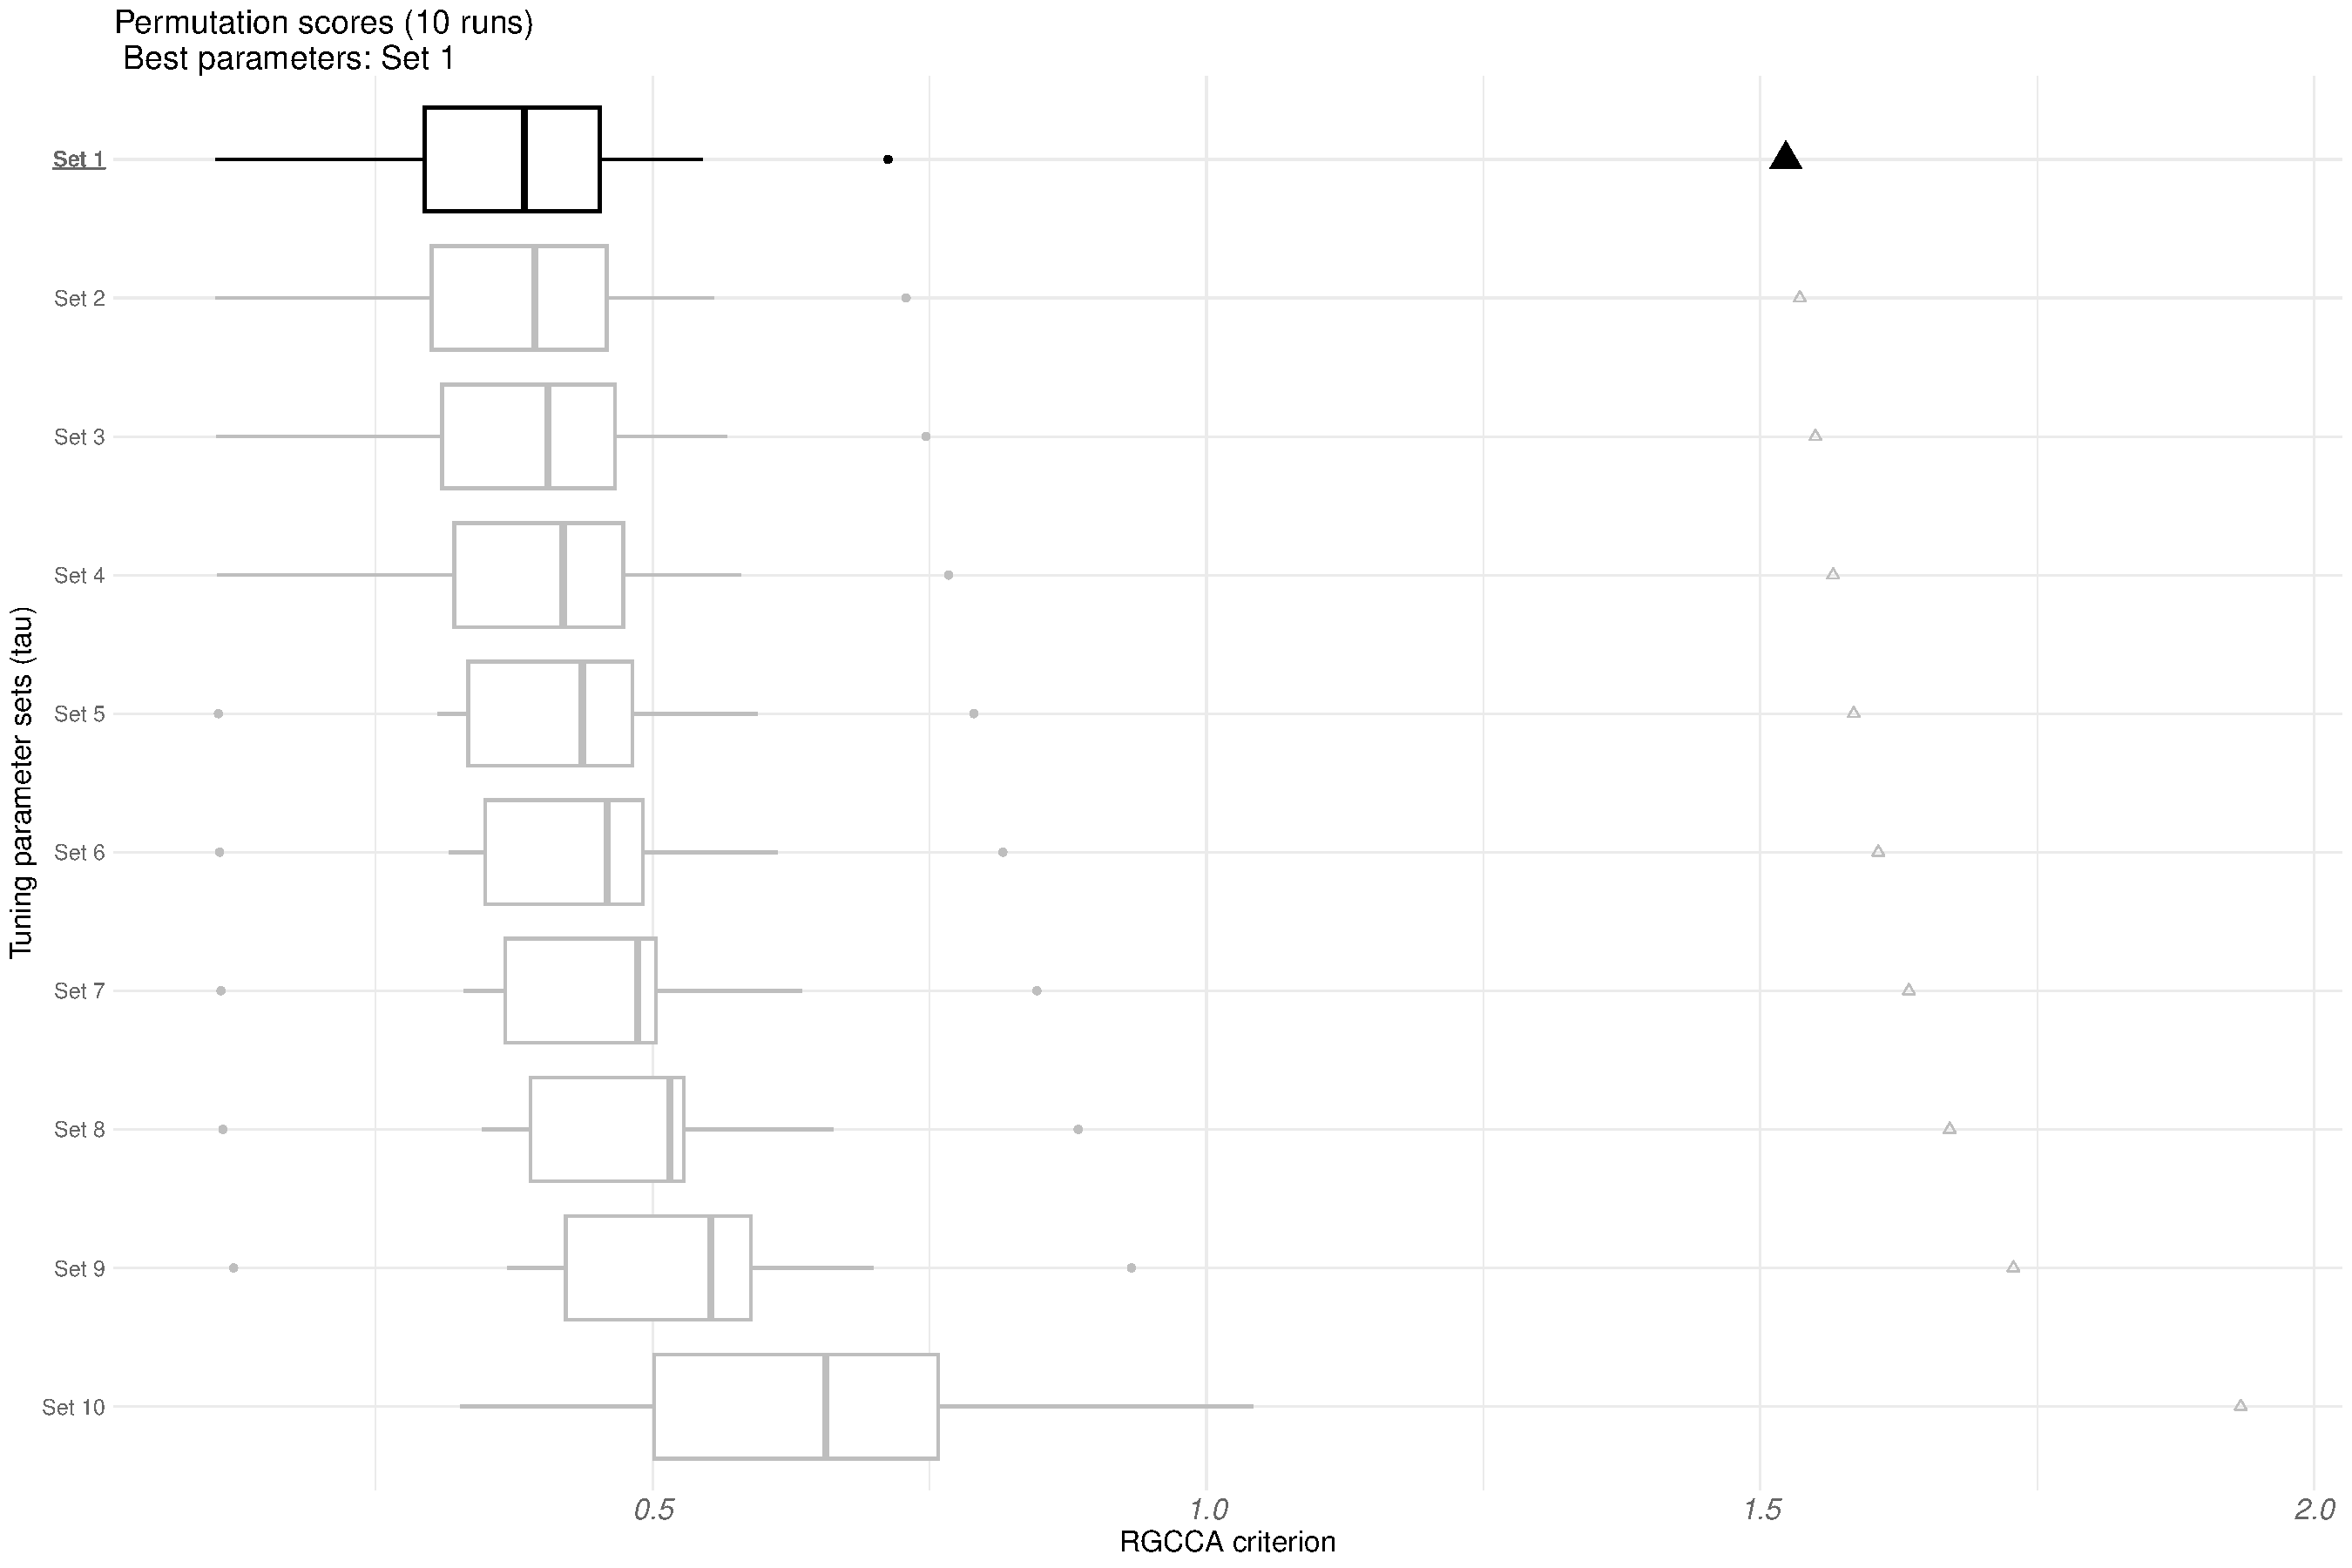
\includegraphics{RGCCA_vignette_files/figure-latex/unnamed-chunk-22-1} \end{center}

\end{CodeChunk}

\normalsize

The fitted permutation object, \texttt{perm\_out}, can be directly
provided as output of \texttt{rgcca()} and visualized/bootstrapped as
usual.

\footnotesize

\begin{CodeChunk}
\begin{CodeInput}
R> fit = rgcca(perm_out)
\end{CodeInput}
\end{CodeChunk}

\normalsize

Of course, it is possible to define explicitly the combination of
regularization parameters to be tested. In that case a matrix of
dimension \(K \times J\) is required. Each row of this matrix
corresponds to one set of tuning parameters.

\footnotesize

\begin{CodeChunk}
\begin{CodeInput}
R> fit.perm = rgcca_permutation(A, connection = C,
+                              par_type = "tau",
+                              par_value = rbind(rep(1, 3),
+                                                seq(0, 1, l=3),
+                                                rep(0, 3),
+                                                sapply(A, RGCCA:::tau.estimate)),
+                              n_cores = 1, n_perms = 5)
\end{CodeInput}
\end{CodeChunk}

\normalsize

Alternatively a numeric vector of length \(J\) indicating the range of
values to be tested: from the minimum values (0 for RGCCA and
\(1/sqrt(ncol)\) for SGCCA) to the maximum values specified by the user
with \texttt{par\_value}.

\footnotesize

\begin{CodeChunk}
\begin{CodeInput}
R> fit.perm = rgcca_permutation(A, connection = C,
+                              par_type = "tau",
+                              par_value = seq(0, 1, l=3),
+                              n_cores = 1, n_perms = 5)
\end{CodeInput}
\end{CodeChunk}

\normalsize

\textbf{Cross-validation strategy.} The optimal tuning parameters can
also be determined by cross-validating different indicators of quality,
namely:

\begin{itemize}
\item
  For Classification: \texttt{Accuracy}, \texttt{Kappa}, \texttt{F1},
  \texttt{Sensitivity}, \texttt{Specificity}, \texttt{Pos\_Pred\_Value},
  \texttt{Neg\_Pred\_Value}, \texttt{Precision}, \texttt{Recall},
  \texttt{Detection\_Rate}, \texttt{Balanced\_Accuracy}.
\item
  For regression: \texttt{RMSE} and \texttt{MAE}.
\end{itemize}

This cross-validation protocol is made available through the
\texttt{rgcca\_cv()} functionand is used here for predicting the
qualitative variable political regime from the two blocks
\texttt{Agriculture\ inequality} and \texttt{Industrial\ development}.

\footnotesize

\begin{CodeChunk}
\begin{CodeInput}
R> blocks <- 
+   list(agriculture = Russett[, seq(3)],
+        industry = Russett[, 4:5],
+        lab = as.matrix(factor(apply(Russett[, 9:11], 1, which.max),
+                        labels = c("Stable", 
+                                   "Unstable",
+                                   "Dictator")))
+                )
R> 
R> set.seed(27) #my favorite number
R> inTraining <- caret:::createDataPartition(blocks[[3]], 
+                                   p = .75, list = FALSE)
R> training <- lapply(blocks, 
+                    function(x) x[inTraining, , drop = FALSE])
R> 
R> testing  <- lapply(blocks, 
+                    function(x) x[-inTraining, , drop = FALSE])
R> 
R> cv_out = rgcca_cv(blocks = training, response = 3, 
+                   par_type = "tau", 
+                   prediction_model = "lda", 
+                   n_run = 10, k = 3,
+                   validation = "kfold", 
+                   ncomp = 1, metric = "Accuracy")
\end{CodeInput}
\end{CodeChunk}

\normalsize

\texttt{rgcca\_cv()} relies on the \texttt{caret} package. As direct
consequence an astonishing large number of models are made available
(see \texttt{caret::modelLookup()}). Results of the cross validation
procedure are reported/displayed using the generic
\texttt{print()/plot()} function

\footnotesize

\begin{CodeChunk}
\begin{CodeInput}
R> print(cv_out)
\end{CodeInput}
\begin{CodeOutput}
Call: method='rgcca', superblock=FALSE, scale=TRUE, scale_block=TRUE, init='svd',
bias=TRUE, tol=1e-08, NA_method='nipals', ncomp=c(1,1,1), response=3,
comp_orth=TRUE 
There are J = 3 blocks.
The design matrix is:
            agriculture industry lab
agriculture           0        0   1
industry              0        0   1
lab                   1        1   0

The factorial scheme is used.

Tuning parameters (tau) used: 
   agriculture industry lab
1        1.000    1.000   0
2        0.889    0.889   0
3        0.778    0.778   0
4        0.667    0.667   0
5        0.556    0.556   0
6        0.444    0.444   0
7        0.333    0.333   0
8        0.222    0.222   0
9        0.111    0.111   0
10       0.000    0.000   0

Validation: kfold with 3 folds and 10 run(s)) 
Prediction model: lda 

   Tuning parameters Mean Accuracy     Sd
1     1.00/1.00/0.00         0.711 0.1043
2     0.89/0.89/0.00         0.714 0.1065
3     0.78/0.78/0.00         0.714 0.1065
4     0.67/0.67/0.00         0.714 0.1065
5     0.56/0.56/0.00         0.722 0.1101
6     0.44/0.44/0.00         0.722 0.1101
7     0.33/0.33/0.00         0.722 0.0987
8     0.22/0.22/0.00         0.719 0.0941
9     0.11/0.11/0.00         0.725 0.0982
10    0.00/0.00/0.00         0.739 0.0922

The best combination is: 0.00/0.00/0.00 for a mean Accuracy of 0.739.
\end{CodeOutput}
\end{CodeChunk}

\normalsize

and displayed using the \texttt{plot()} function.

\footnotesize

\begin{CodeChunk}
\begin{CodeInput}
R> plot(cv_out, cex = 1.3)
\end{CodeInput}


\begin{center}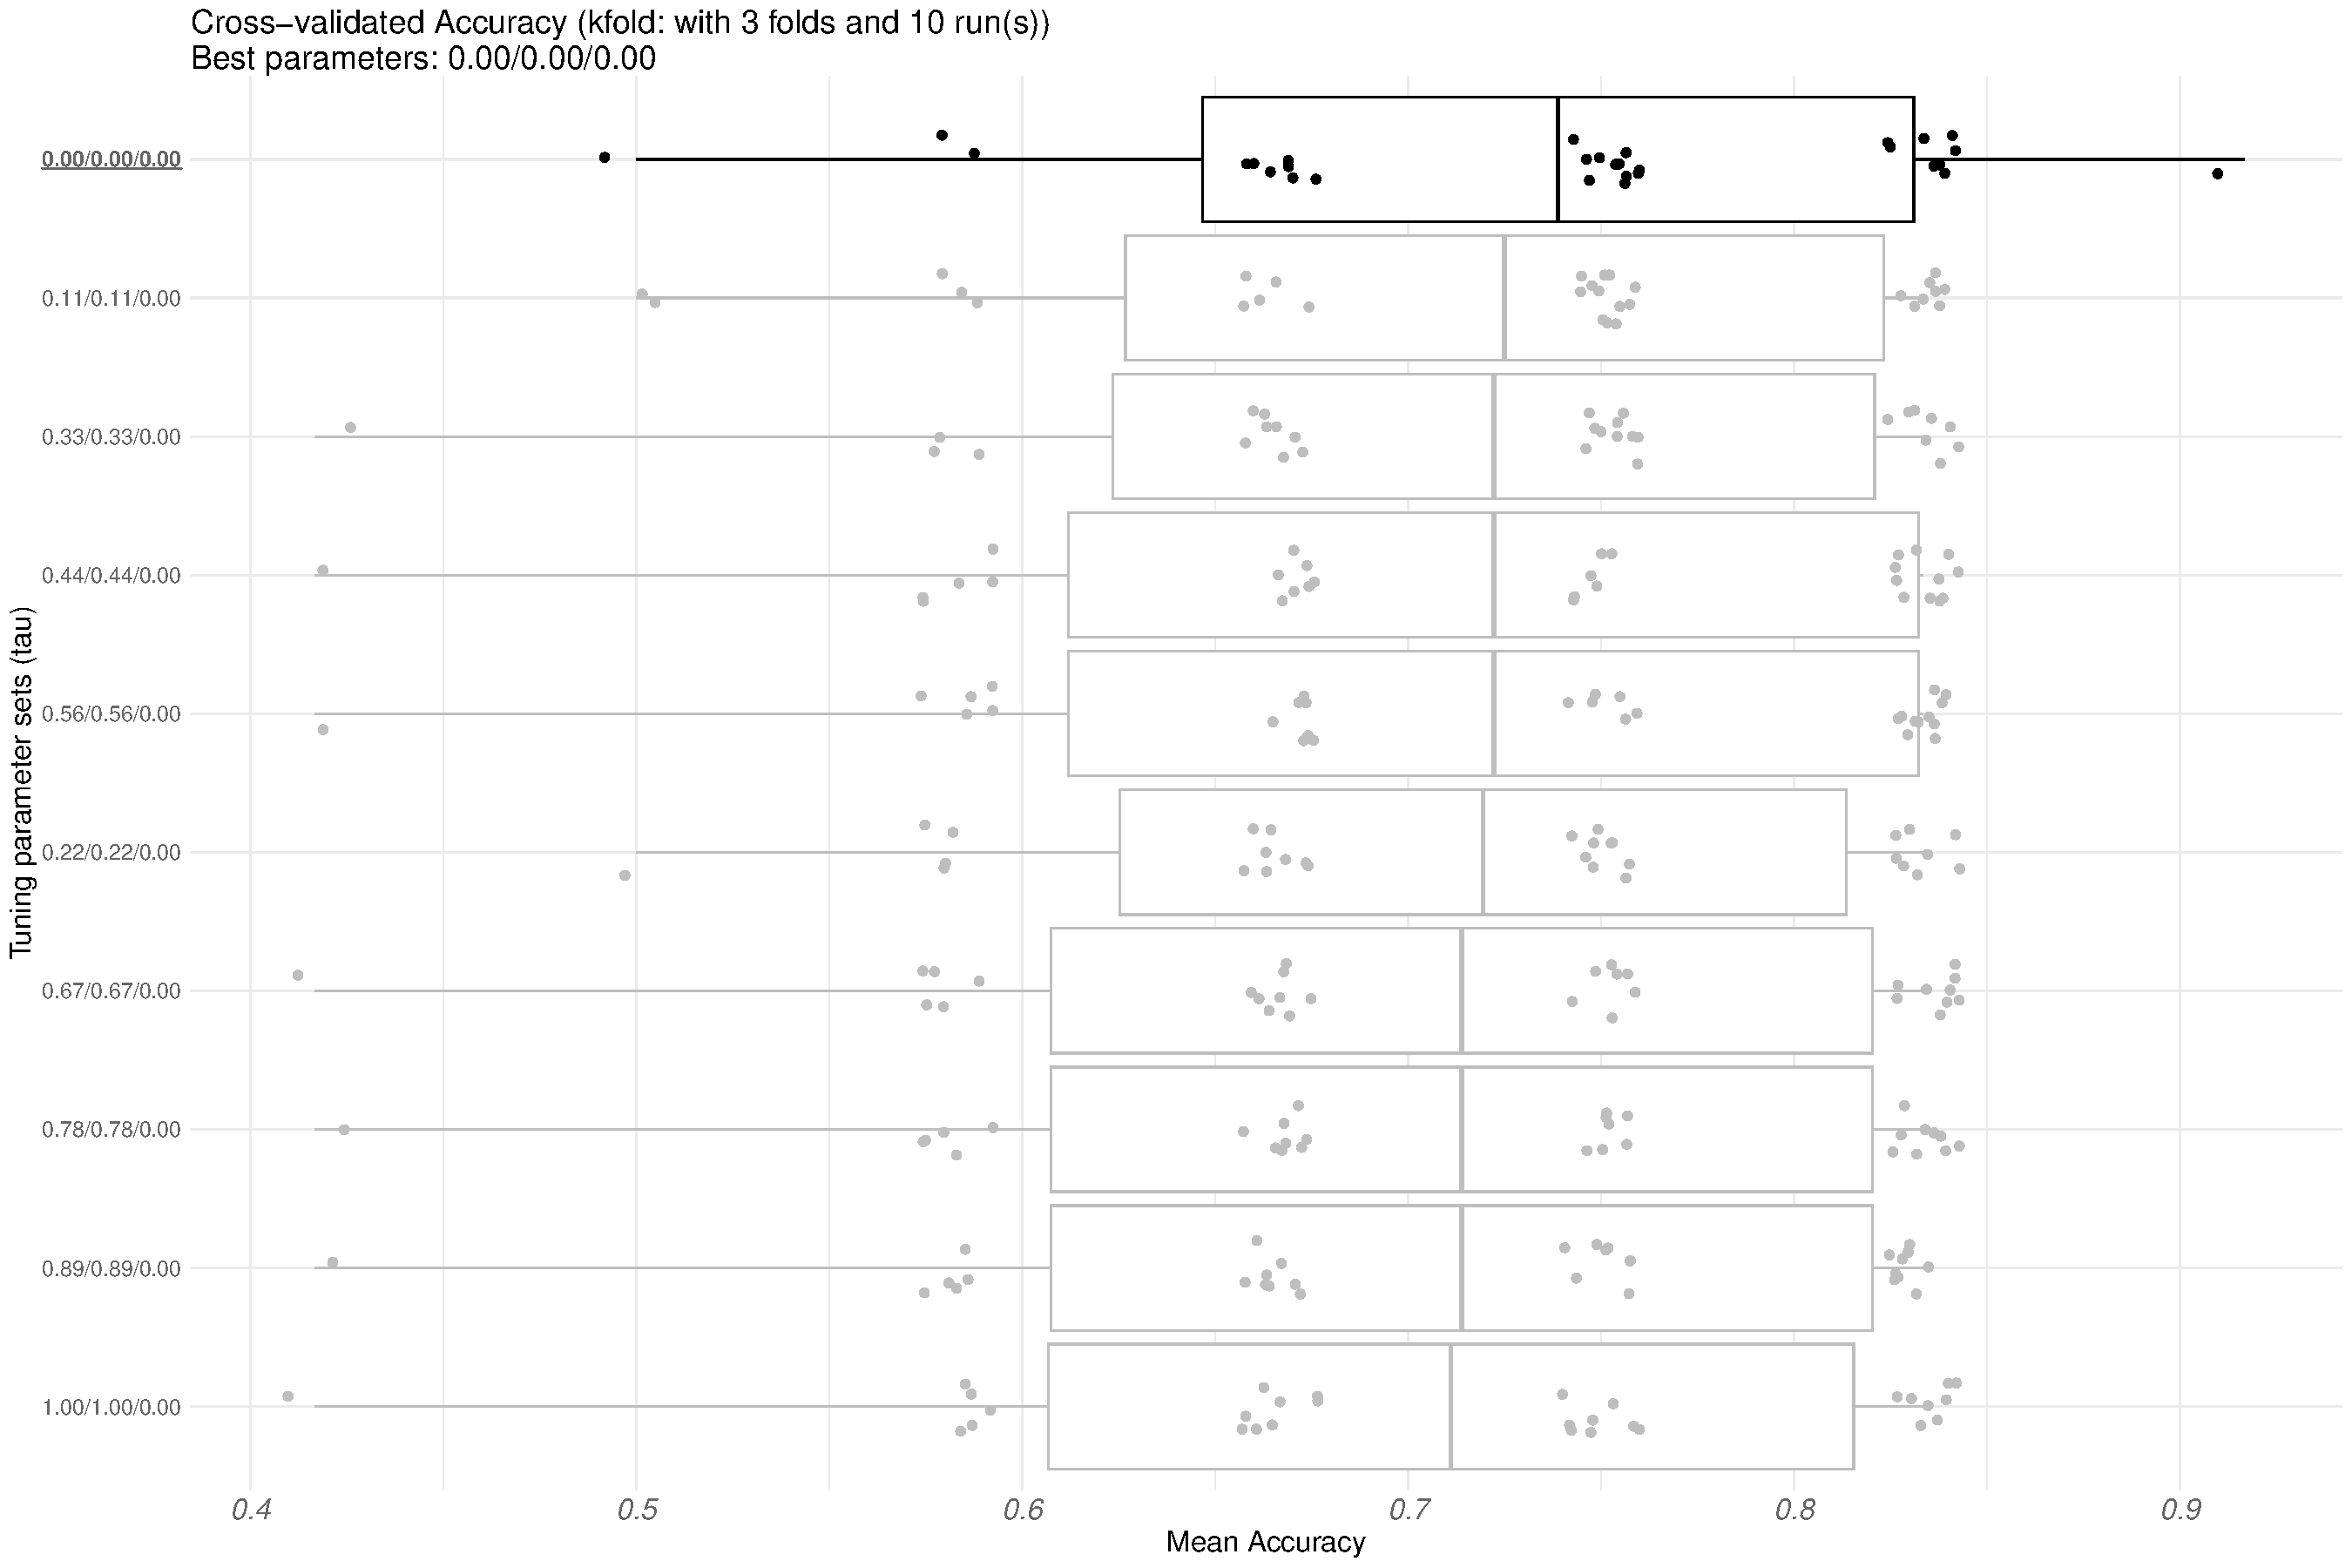
\includegraphics{RGCCA_vignette_files/figure-latex/unnamed-chunk-28-1} \end{center}

\end{CodeChunk}

\normalsize

The fitted cval object can be provided as output of \texttt{rgcca()} and
the resulting optimal model can be visualized/bootstrapped as usual.

\footnotesize

\begin{CodeChunk}
\begin{CodeInput}
R> fit = rgcca(cv_out)
\end{CodeInput}
\end{CodeChunk}

\normalsize

At last, \texttt{rgcca\_predict()} can be used for predicting new
blocks.

\footnotesize

\begin{CodeChunk}
\begin{CodeInput}
R> perf = rgcca_predict(fit, blocks_test = testing, prediction_model = "lda")
\end{CodeInput}
\end{CodeChunk}

\normalsize

and a \texttt{caret} summary of the performances be reported

\footnotesize

\begin{CodeChunk}
\begin{CodeInput}
R> perf$confusion$test
\end{CodeInput}
\begin{CodeOutput}
Confusion Matrix and Statistics

          Reference
Prediction Dictator Stable Unstable
  Dictator        5      0        2
  Stable          0      3        1
  Unstable        0      0        0

Overall Statistics
                                          
               Accuracy : 0.7273          
                 95% CI : (0.3903, 0.9398)
    No Information Rate : 0.4545          
    P-Value [Acc > NIR] : 0.06478         
                                          
                  Kappa : 0.5541          
                                          
 Mcnemar's Test P-Value : NA              

Statistics by Class:

                     Class: Dictator Class: Stable Class: Unstable
Sensitivity                   1.0000        1.0000          0.0000
Specificity                   0.6667        0.8750          1.0000
Pos Pred Value                0.7143        0.7500             NaN
Neg Pred Value                1.0000        1.0000          0.7273
Prevalence                    0.4545        0.2727          0.2727
Detection Rate                0.4545        0.2727          0.0000
Detection Prevalence          0.6364        0.3636          0.0000
Balanced Accuracy             0.8333        0.9375          0.5000
\end{CodeOutput}
\end{CodeChunk}

\normalsize

All the functions presented previously are designed for sparse analysis.
This will be illustrated in the next section.

\hypertarget{high-dimensional-case-study-glioma-data}{%
\section{High dimensional case study: Glioma
Data}\label{high-dimensional-case-study-glioma-data}}

\textbf{Biological problem.} Brain tumors are the most common solid
tumors in children and have the highest mortality rate of all pediatric
cancers. Despite advances in multimodality therapy, children with pHGG
invariably have an overall survival of around 20\% at 5 years. Depending
on their location (e.g.~brainstem, central nuclei, or supratentorial),
pHGG present different characteristics in terms of radiological
appearance, histology, and prognosis. Our hypothesis is that pHGG have
different genetic origins and oncogenic pathways depending on their
location. Thus, the biological processes involved in the development of
the tumor may be different from one location to another, as it has been
frequently suggested.

\textbf{Description of the data.} Pretreatment frozen tumor samples were
obtained from 53 children with newly diagnosed pHGG from Necker Enfants
Malades (Paris, France) \citep{Puget2012}. The 53 tumors are divided
into 3 locations: supratentorial (HEMI), central nuclei (MIDL), and
brain stem (DIPG). The final dataset is organized in 3 blocks of
variables defined for the 53 tumors: the first block \(\mathbf{X}_1\)
provides the expression of \(15702\) genes (GE). The second block
\(\mathbf{X}_2\) contains the imbalances of \(1229\) segments (CGH) of
chromosomes. \(\mathbf{X}_3\) is a block of dummy variables describing
the categorical variable location. One dummy variable has been left out
because of redundancy with the others.

\footnotesize

\begin{CodeChunk}
\begin{CodeInput}
R> # Download the dataset's package at http://biodev.cea.fr/sgcca/.
R> # --> gliomaData_0.4.tar.gz
R> 
R> require(gliomaData)
\end{CodeInput}
\begin{CodeOutput}
Loading required package: gliomaData
\end{CodeOutput}
\begin{CodeInput}
R> data(ge_cgh_locIGR)
R> 
R> blocks <- ge_cgh_locIGR$multiblocks
R> Loc <- factor(ge_cgh_locIGR$y)
R> levels(Loc) <- colnames(ge_cgh_locIGR$multiblocks$y)
R> blocks[[3]] = Loc
R> 
R> # check dimensions of the blocks
R> sapply(blocks, NCOL)
\end{CodeInput}
\begin{CodeOutput}
   GE   CGH     y 
15702  1229     1 
\end{CodeOutput}
\end{CodeChunk}

\normalsize

We impose \(\mathbf{X}_1\) and \(\mathbf{X}_2\) to be connected to
\(\mathbf{X}_3\). This design is commonly used in many applications and
is oriented toward the prediction of the location. The argument
\texttt{response=3} of the \texttt{rgcca()} function encodes this
design.

\footnotesize

\begin{CodeChunk}
\begin{CodeInput}
R> fit.rgcca = rgcca(blocks = blocks, response = 3, ncomp = 2, verbose = TRUE)
\end{CodeInput}
\begin{CodeOutput}
Computation of the RGCCA block components based on the factorial scheme 
Shrinkage intensity parameters are chosen manually 
Computation of the RGCCA block components #1 is under progress...
 Iter:    1  Fit:  0.13465500  Dif:  0.12507270 
 Iter:    2  Fit:  0.15313643  Dif:  0.01848143 
 Iter:    3  Fit:  0.15844550  Dif:  0.00530907 
 Iter:    4  Fit:  0.15963587  Dif:  0.00119037 
 Iter:    5  Fit:  0.15988694  Dif:  0.00025107 
 Iter:    6  Fit:  0.15993920  Dif:  0.00005226 
 Iter:    7  Fit:  0.15995005  Dif:  0.00001085 
 Iter:    8  Fit:  0.15995230  Dif:  0.00000225 
 Iter:    9  Fit:  0.15995277  Dif:  0.00000047 
 Iter:   10  Fit:  0.15995286  Dif:  0.00000010 
 Iter:   11  Fit:  0.15995288  Dif:  0.00000002 
 Iter:   12  Fit:  0.15995289  Dif:  0.00000000 
\end{CodeOutput}
\begin{CodeOutput}
The RGCCA algorithm converged to a stationary point after 11 iterations 
\end{CodeOutput}
\begin{CodeOutput}
Computation of the RGCCA block components #2 is under progress...
 Iter:    1  Fit:  0.06987951  Dif:  0.06715811 
 Iter:    2  Fit:  0.07066188  Dif:  0.00078237 
 Iter:    3  Fit:  0.07073615  Dif:  0.00007427 
 Iter:    4  Fit:  0.07074309  Dif:  0.00000694 
 Iter:    5  Fit:  0.07074374  Dif:  0.00000065 
 Iter:    6  Fit:  0.07074380  Dif:  0.00000006 
 Iter:    7  Fit:  0.07074380  Dif:  0.00000001 
\end{CodeOutput}
\begin{CodeOutput}
The RGCCA algorithm converged to a stationary point after 6 iterations 
\end{CodeOutput}


\begin{center}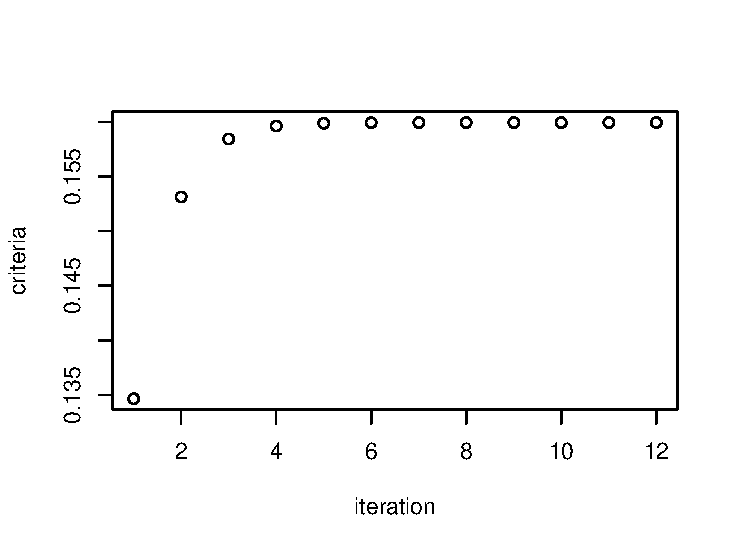
\includegraphics{RGCCA_vignette_files/figure-latex/unnamed-chunk-33-1} \end{center}



\begin{center}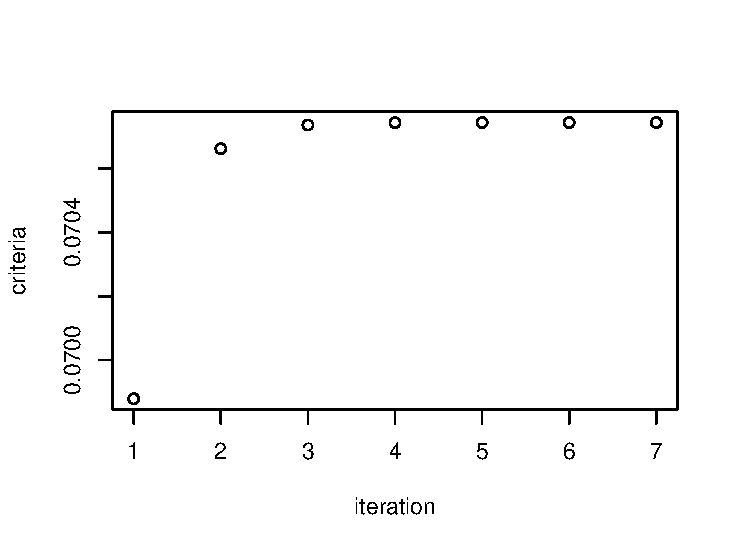
\includegraphics{RGCCA_vignette_files/figure-latex/unnamed-chunk-33-2} \end{center}

\end{CodeChunk}

\normalsize

When the response variable is qualitative, two steps are implicitly
performed: (i) disjunctive coding and (ii) the associated shrinkage
parameter is set to \(0\) regardless of the value specified by the user.

\footnotesize

\begin{CodeChunk}
\begin{CodeInput}
R> fit.rgcca$call$connection
\end{CodeInput}
\begin{CodeOutput}
    GE CGH y
GE   0   0 1
CGH  0   0 1
y    1   1 0
\end{CodeOutput}
\begin{CodeInput}
R> fit.rgcca$call$tau
\end{CodeInput}
\begin{CodeOutput}
[1] 1 1 0
\end{CodeOutput}
\end{CodeChunk}

\normalsize

From the dimension of each block (\(n>p\) or \(n\leq p\)),
\texttt{rgcca()} selects automatically the dual formulation for
\(\mathbf{X}_1\) and \(\mathbf{X}_2\) and the primal one for
\(\mathbf{X}_3\). The formulation used for each block is returned using
the following command:

\footnotesize

\begin{CodeChunk}
\begin{CodeInput}
R> fit.rgcca$primal_dual
\end{CodeInput}
\begin{CodeOutput}
[1] "dual"   "dual"   "primal"
\end{CodeOutput}
\end{CodeChunk}

\normalsize

The dual formulation make the RGCCA algorithm highly efficient even in a
high dimensional setting.

\footnotesize

\begin{CodeChunk}
\begin{CodeInput}
R> system.time(
+   rgcca(blocks = blocks, response = 3)
+ )
\end{CodeInput}
\begin{CodeOutput}
   user  system elapsed 
   1.66    0.00    1.68 
\end{CodeOutput}
\end{CodeChunk}

\normalsize

RGCCA enables visual inspection of the spatial relationships between
classes. This facilitates assessment of the quality of the
classification and makes it possible to readily determine which
components capture the discriminant information.

\footnotesize

\begin{CodeChunk}
\begin{CodeInput}
R> plot(fit.rgcca, type = "sample", block=1:2,
+      comp = 1, response = Loc)
\end{CodeInput}


\begin{center}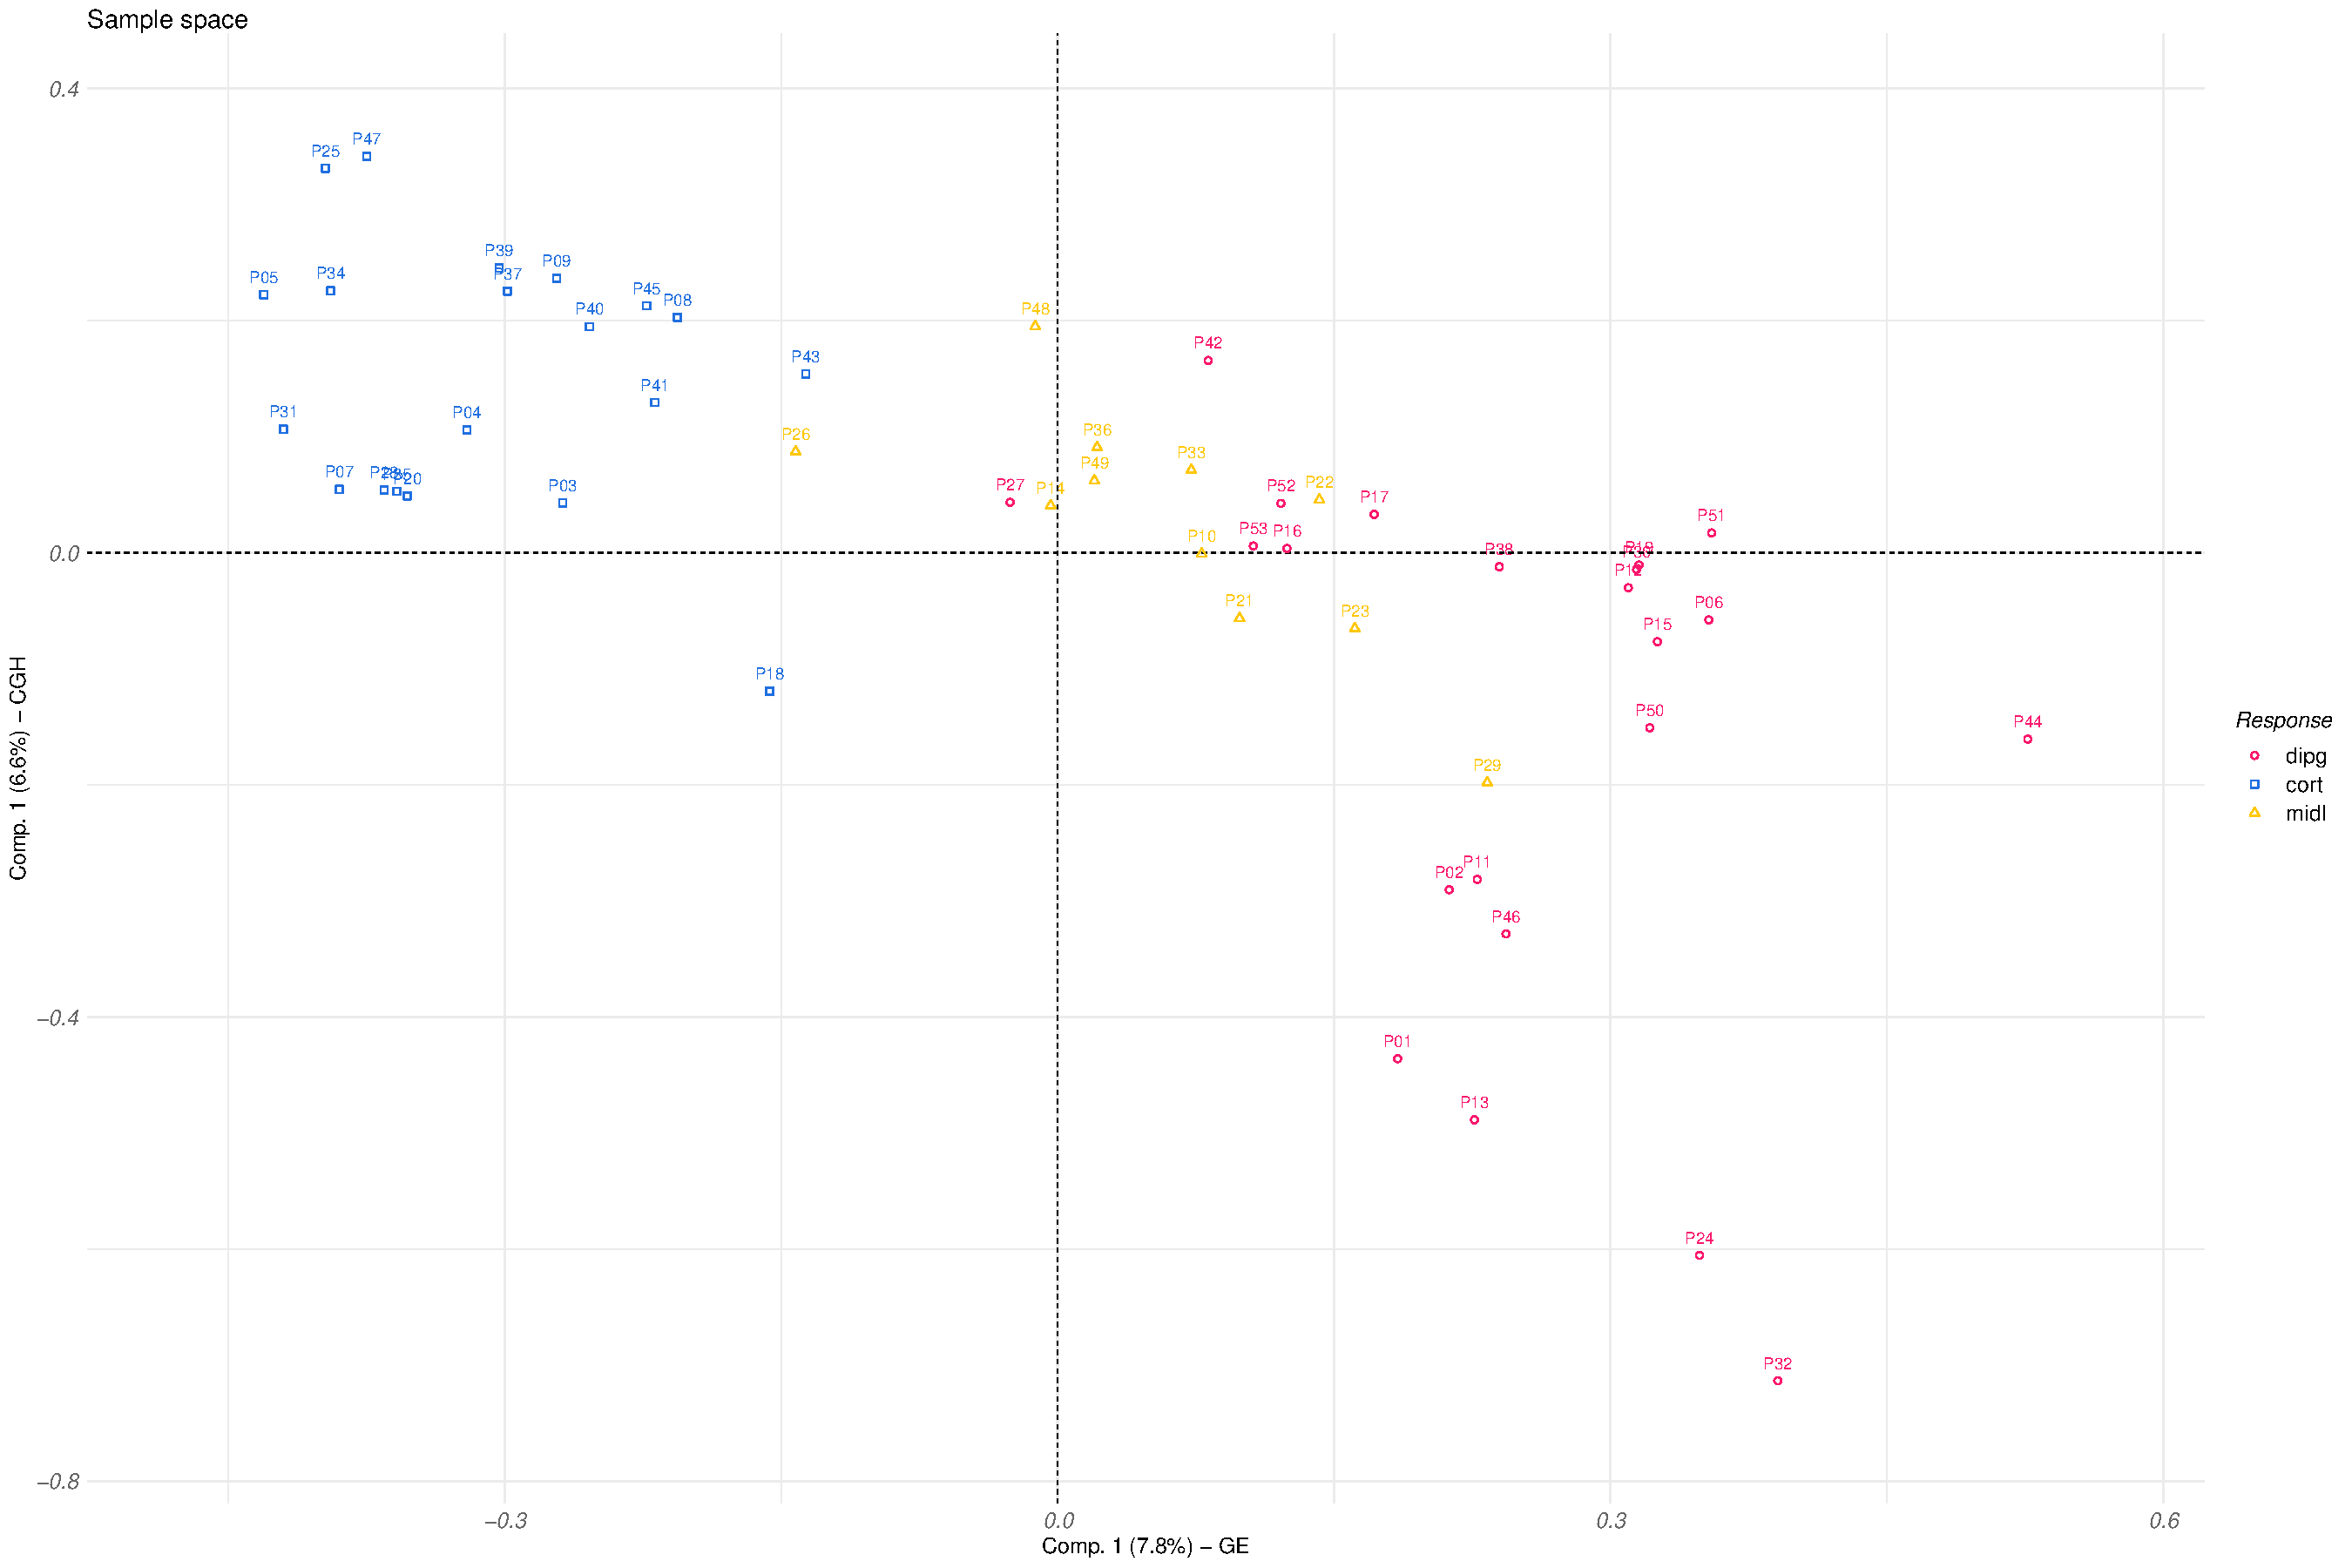
\includegraphics{RGCCA_vignette_files/figure-latex/unnamed-chunk-37-1} \end{center}

\end{CodeChunk}

\normalsize

For easier interpretation of the results, especially in high-dimensional
settings, it is often appropriate to add, within the RGCCA optimization
problem, penalties promoting sparsity. For that purpose, an \(\ell_1\)
penalization on the weight vectors
\(\mathbf{a}_1, \ldots, \mathbf{a}_J\) is applied. the \texttt{sparsity}
argument of \texttt{rgcca()} varies between 1/sqrt(ncol) and 1 (larger
values of \texttt{sparsity} correspond to less penalization) and control
the amount of sparsity of the weight vectors
\(\mathbf{a}_1, \ldots, \mathbf{a}_J\). If \texttt{sparsity} is a
vector, \(\ell_1\)-penalties are the same for all the weights
corresponding to the same block but different components:

\begin{equation}
\forall h, \Vert \mathbf{a}_j^{(h)} \Vert_{\ell_1} \leq c_{1j} \sqrt{p_j},
\end{equation}

with \(p_j\) the number of variables of \(\X_j\).

If \texttt{sparsity} is a matrix, row \(h\) of \texttt{sparsity} defines
the constraints applied to the weights corresponding to components
\(h\):

\begin{equation}
\forall h, \Vert \mathbf{a}_j^{(h)} \Vert_{\ell_1} \leq c_1[h,j] \sqrt{p_j}.
\end{equation}

\hypertarget{sgcca-for-the-glioma-dataset}{%
\subsection{SGCCA for the Glioma
dataset}\label{sgcca-for-the-glioma-dataset}}

The algorithm associated with the optimization problem
(\ref{optim_SGCCA}) is available through the function \texttt{rgcca()}
with the argument \texttt{method="sgcca"}.

\footnotesize

\begin{CodeChunk}
\begin{CodeInput}
R> fit.sgcca = rgcca(blocks = blocks, response = 3, ncomp = 2, 
+                   sparsity = c(0.0710, 0.2000, 1),
+                   verbose = TRUE)
\end{CodeInput}
\begin{CodeOutput}
Computation of the SGCCA block components based on the factorial scheme 
Computation of the SGCCA block components #1 is under progress...
 Iter:    1  Fit:  0.01102201  Dif:  0.01084380 
 Iter:    2  Fit:  0.01185962  Dif:  0.00083761 
 Iter:    3  Fit:  0.01251465  Dif:  0.00065502 
 Iter:    4  Fit:  0.01280624  Dif:  0.00029159 
 Iter:    5  Fit:  0.01286779  Dif:  0.00006155 
 Iter:    6  Fit:  0.01288261  Dif:  0.00001483 
 Iter:    7  Fit:  0.01288695  Dif:  0.00000434 
 Iter:    8  Fit:  0.01288830  Dif:  0.00000135 
 Iter:    9  Fit:  0.01288872  Dif:  0.00000043 
 Iter:   10  Fit:  0.01288886  Dif:  0.00000014 
 Iter:   11  Fit:  0.01288891  Dif:  0.00000004 
 Iter:   12  Fit:  0.01288892  Dif:  0.00000001 
 Iter:   13  Fit:  0.01288893  Dif:  0.00000000 
\end{CodeOutput}
\begin{CodeOutput}
The SGCCA algorithm converged to a stationary point after 12 iterations 
\end{CodeOutput}
\begin{CodeOutput}
Computation of the SGCCA block components #2 is under progress...
 Iter:    1  Fit:  0.00649703  Dif:  0.00645637 
 Iter:    2  Fit:  0.00879433  Dif:  0.00229731 
 Iter:    3  Fit:  0.00905191  Dif:  0.00025758 
 Iter:    4  Fit:  0.00906832  Dif:  0.00001641 
 Iter:    5  Fit:  0.00906923  Dif:  0.00000090 
 Iter:    6  Fit:  0.00906928  Dif:  0.00000005 
 Iter:    7  Fit:  0.00906928  Dif:  0.00000000 
\end{CodeOutput}
\begin{CodeOutput}
The SGCCA algorithm converged to a stationary point after 6 iterations 
\end{CodeOutput}


\begin{center}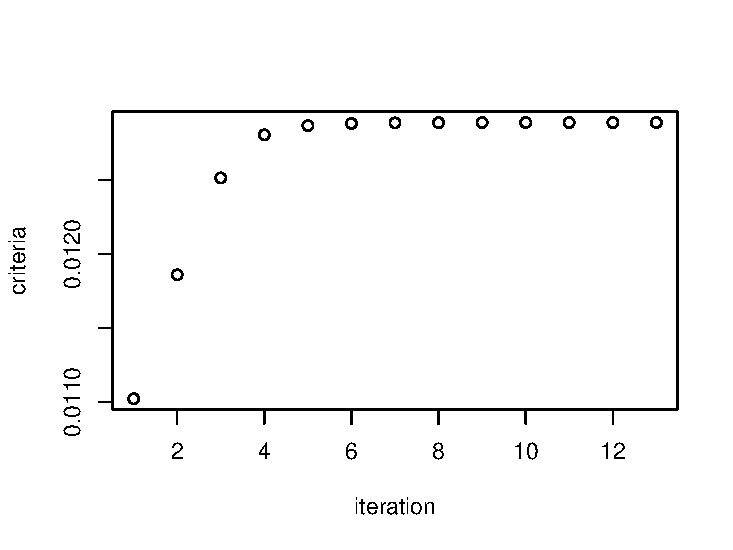
\includegraphics{RGCCA_vignette_files/figure-latex/unnamed-chunk-38-1} \end{center}



\begin{center}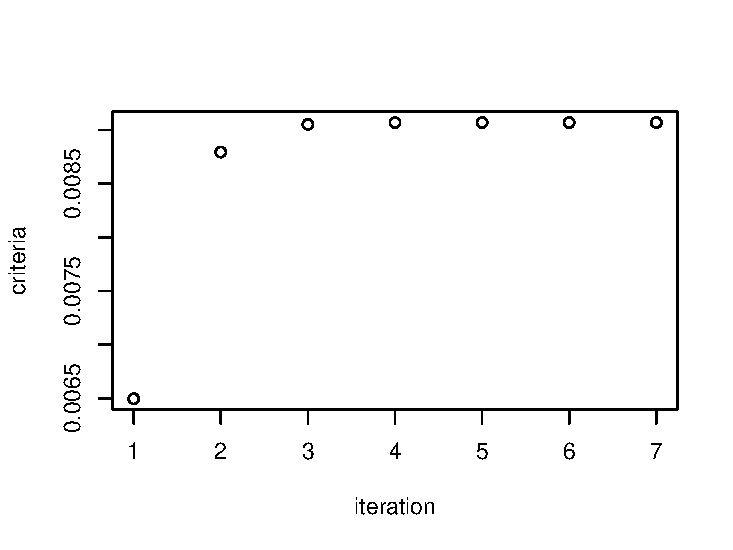
\includegraphics{RGCCA_vignette_files/figure-latex/unnamed-chunk-38-2} \end{center}

\end{CodeChunk}

\normalsize

the \texttt{print()} function allows summarizing the SGCCA analysis.

\footnotesize

\begin{CodeChunk}
\begin{CodeInput}
R> print(fit.sgcca)
\end{CodeInput}
\begin{CodeOutput}
Call: method='sgcca', superblock=FALSE, scale=TRUE, scale_block='inertia',
init='svd', bias=TRUE, tol=1e-08, NA_method='nipals', ncomp=c(2,2,2),
response=3, comp_orth=TRUE 
There are J = 3 blocks.
The design matrix is:
    GE CGH y
GE   0   0 1
CGH  0   0 1
y    1   1 0

The factorial scheme is used.
Sum_{j,k} c_jk g(cov(X_j a_j, X_k a_k) = 0.022 

The sparsity parameter used for GE is: 0.071 (with 146, 145 variables selected)
The sparsity parameter used for CGH is: 0.2 (with 84, 76 variables selected)
The regularization parameter used for y is: 0
\end{CodeOutput}
\end{CodeChunk}

\normalsize

and the \texttt{plot()} returns the same graphical displays as RGCCA. We
skip these representations for sake of brevity.

In this situation, the optimal sparsity parameters is usually chosen by
cross-validation using the \texttt{rgcca\_cv()} function. The goal is to
maximize the cross-validated accuracy (\texttt{metric\ =\ Accuracy}) in
a model where we try to predict the response block from all the block
components with a user-defined classifier (\texttt{prediction\_model}).
also, we decide to upper bound the sparsity parameters for \(X_1\) and
\(X_2\) to \(0.2\), to achieve an attractive amount of sparsity.

\footnotesize

\begin{CodeChunk}
\begin{CodeInput}
R> set.seed(27) #my favorite number
R> cv_out <- rgcca_cv(blocks, response = 3, 
+                    par_type = "sparsity",
+                    par_value = c(.2, .2, 0), 
+                    par_length = 10, 
+                    prediction_model = "lda",
+                    validation = "kfold",
+                    k = 3, n_run = 10, metric = "Accuracy",
+                    n_cores = 15)
\end{CodeInput}
\end{CodeChunk}

\normalsize

We can report the results of this cross-validation using the generic
\texttt{print()} and \texttt{plot()} functions and build the optimal
model using the fitted \texttt{cval} object as argument of
\texttt{rgcca()}:

\footnotesize

\begin{CodeChunk}
\begin{CodeInput}
R> print(cv_out)
\end{CodeInput}
\begin{CodeOutput}
Call: method='sgcca', superblock=FALSE, scale=TRUE, scale_block=TRUE, init='svd',
bias=TRUE, tol=1e-08, NA_method='nipals', ncomp=c(1,1,1), response=3,
comp_orth=TRUE 
There are J = 3 blocks.
The design matrix is:
    GE CGH y
GE   0   0 1
CGH  0   0 1
y    1   1 0

The factorial scheme is used.

Tuning parameters (sparsity) used: 
      GE   CGH y
1  0.200 0.200 0
2  0.179 0.181 0
3  0.157 0.162 0
4  0.136 0.143 0
5  0.115 0.124 0
6  0.093 0.105 0
7  0.072 0.086 0
8  0.051 0.067 0
9  0.029 0.048 0
10 0.008 0.029 0

Validation: kfold with 3 folds and 10 run(s)) 
Prediction model: lda 

   Tuning parameters Mean Accuracy     Sd
1              Set 1         0.760 0.0598
2              Set 2         0.760 0.0615
3              Set 3         0.760 0.0613
4              Set 4         0.774 0.0690
5              Set 5         0.777 0.0840
6              Set 6         0.771 0.0844
7              Set 7         0.747 0.1329
8              Set 8         0.748 0.1386
9              Set 9         0.664 0.1937
10            Set 10         0.567 0.1674

The best combination is: Set 5 for a mean Accuracy of 0.777.
\end{CodeOutput}
\end{CodeChunk}

\normalsize

\footnotesize

\begin{CodeChunk}
\begin{CodeInput}
R> plot(cv_out)
\end{CodeInput}


\begin{center}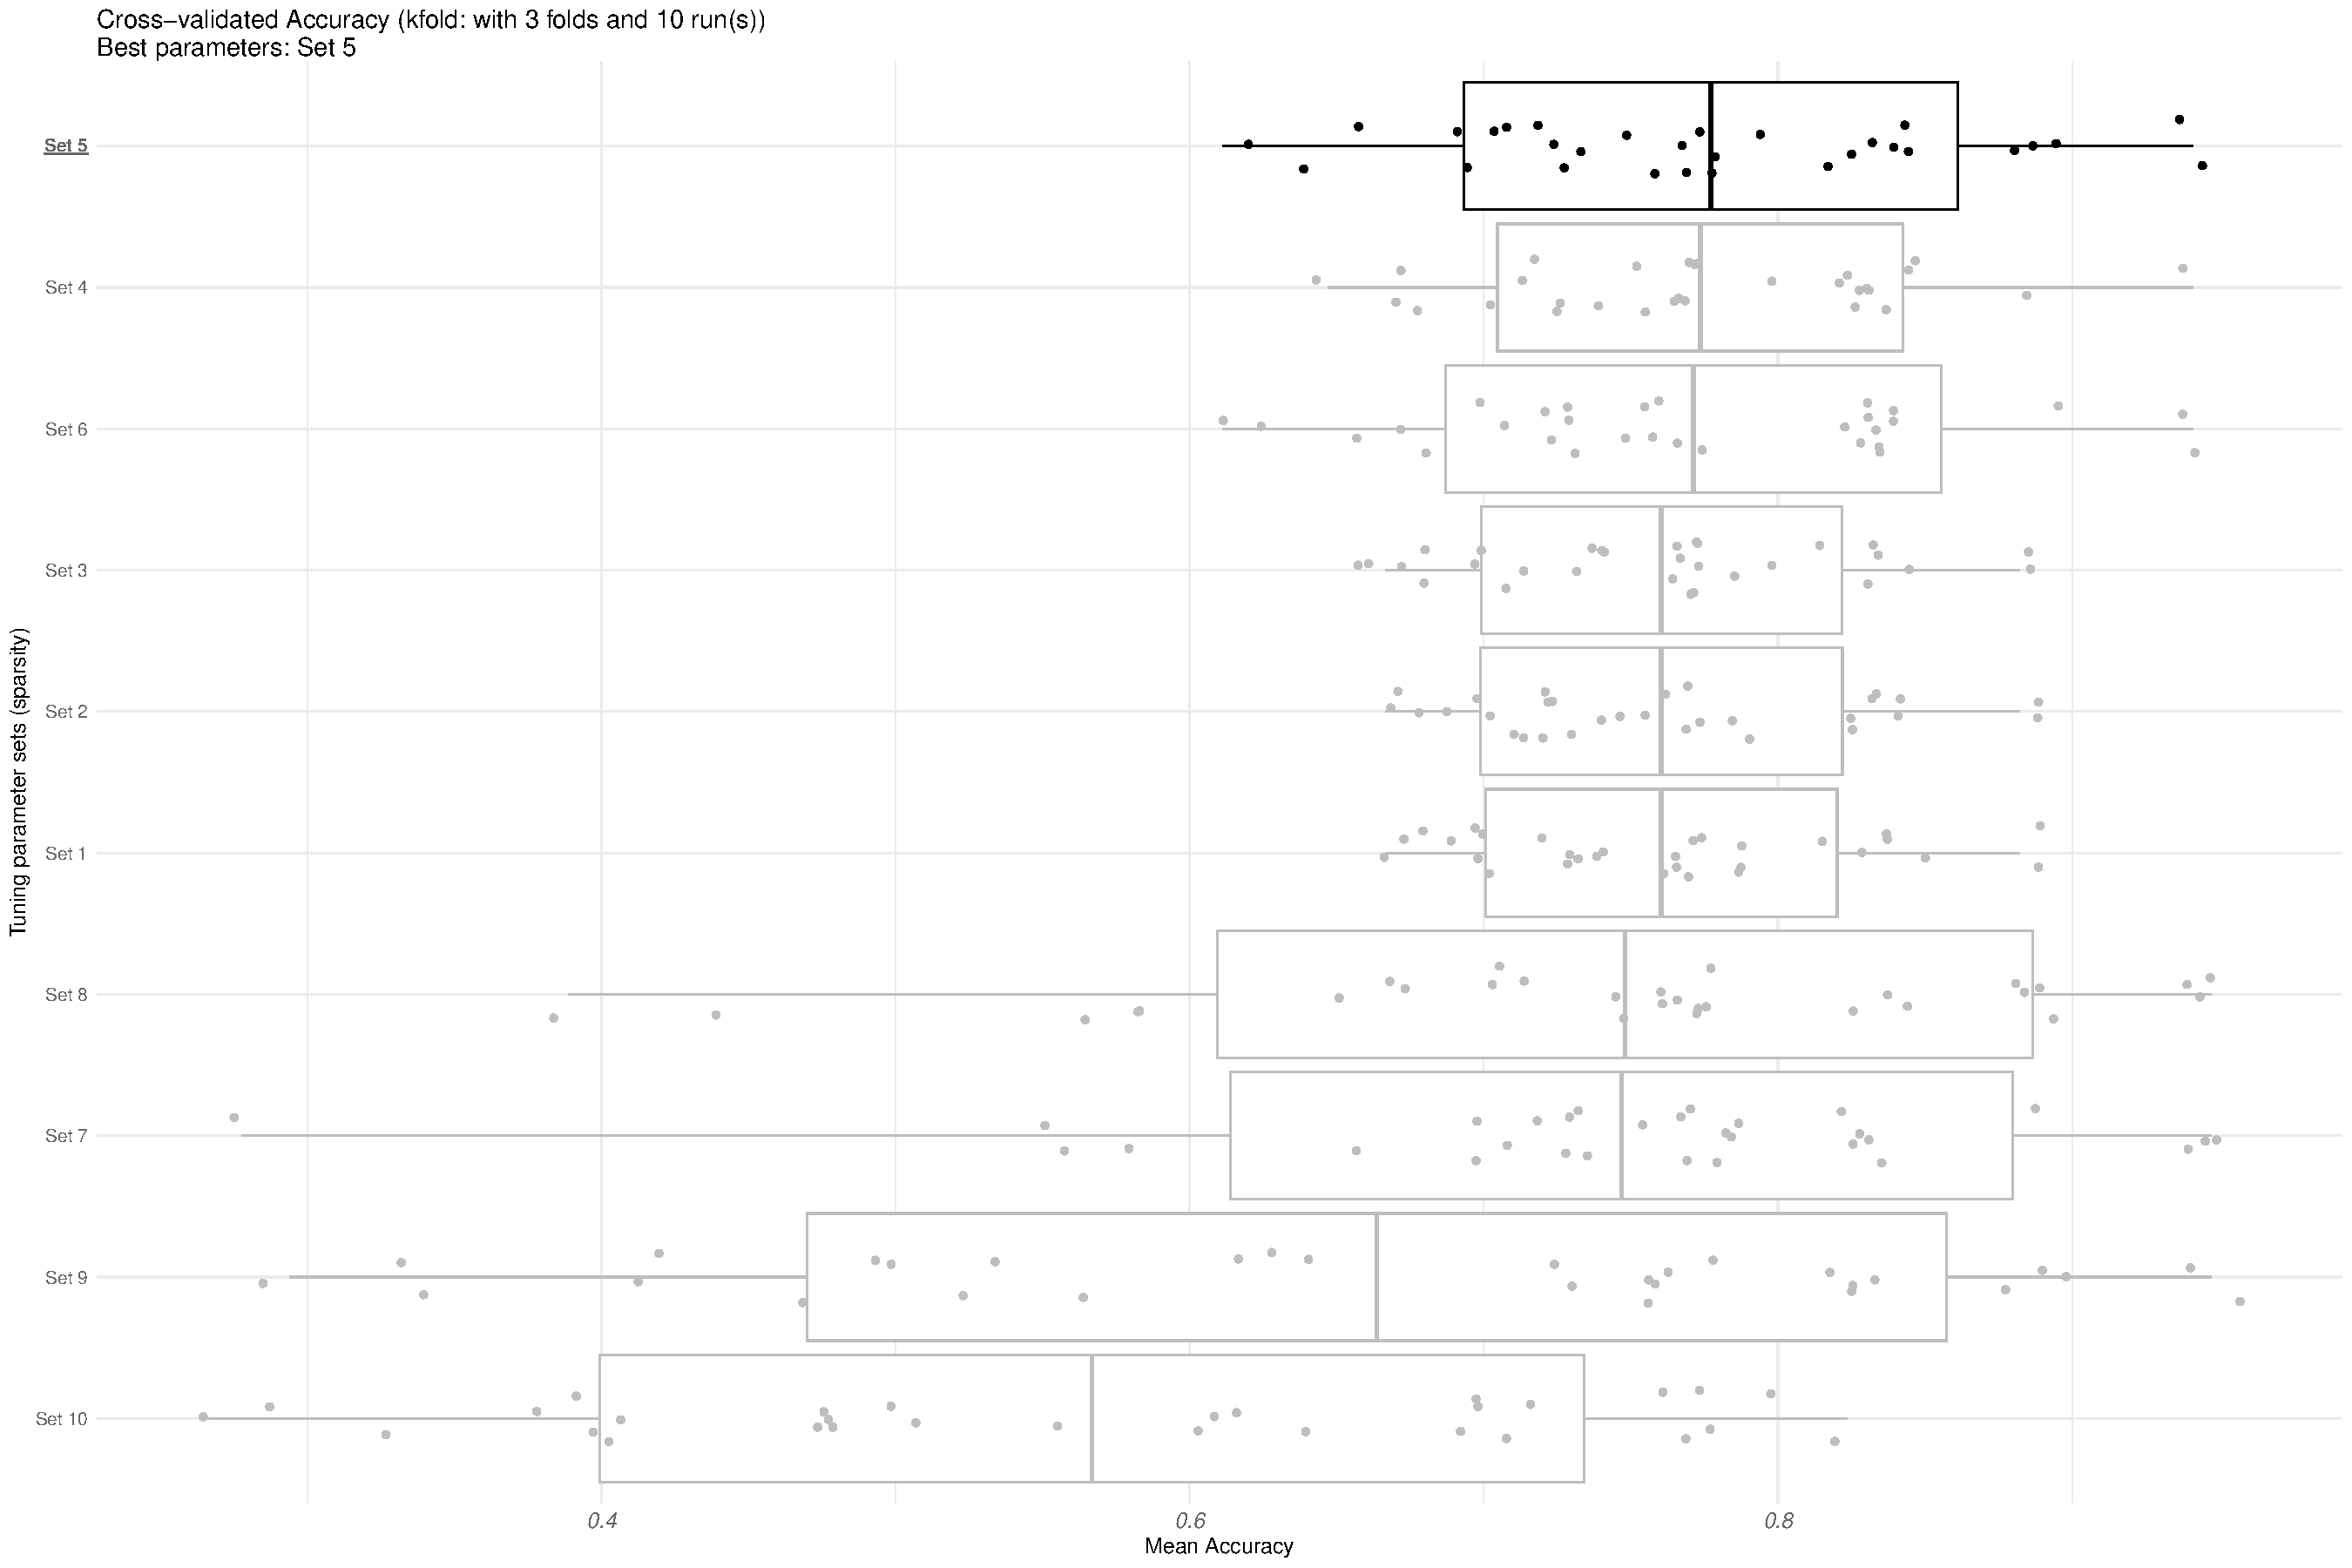
\includegraphics{RGCCA_vignette_files/figure-latex/unnamed-chunk-42-1} \end{center}

\end{CodeChunk}

\normalsize

\footnotesize

\begin{CodeChunk}
\begin{CodeInput}
R> fit = rgcca(cv_out)
\end{CodeInput}
\end{CodeChunk}

\normalsize

Notice that the sparsity parameter associated with \(\mathbf{X}_3\)
switches automatically to regularization parameter set to
\(\tau_3 = 0\). This choice is justified by the fact that we were not
looking for a block component \(\y_3\) that explained its own block well
(since \(\mathbf{X}_3\) is a group coding matrix) but one that
correlated with its neighboring components.

Also it is possible to stabilize the selected variables using the
\texttt{rgcca\_stability()} function.

\footnotesize

\begin{CodeChunk}
\begin{CodeInput}
R> fit_stab = rgcca_stability(fit, 
+                            keep = sapply(fit$a, 
+                                          function(x) mean(x!=0)),
+                            n_boot = 100, verbose = TRUE, n_cores = 15)
\end{CodeInput}
\end{CodeChunk}

\normalsize

and then apply the bootstrap procedure on the most stable variables.

\footnotesize

\begin{CodeChunk}
\begin{CodeInput}
R> boot_out = rgcca_bootstrap(fit_stab, n_boot = 500)
\end{CodeInput}
\begin{CodeOutput}
All the parameters were imported from the fitted rgcca_stability object.
\end{CodeOutput}
\begin{CodeOutput}
Bootstrap samples sanity check...OK
\end{CodeOutput}
\end{CodeChunk}

\normalsize

The bootstrap results can be visualized using the generic
\texttt{plot()} function.

\footnotesize

\begin{CodeChunk}
\begin{CodeInput}
R> plot(boot_out, block = 1:2, 
+      display_order = FALSE, 
+      n_mark = 2000, cex = 1.3, 
+      show_star = FALSE)
\end{CodeInput}


\begin{center}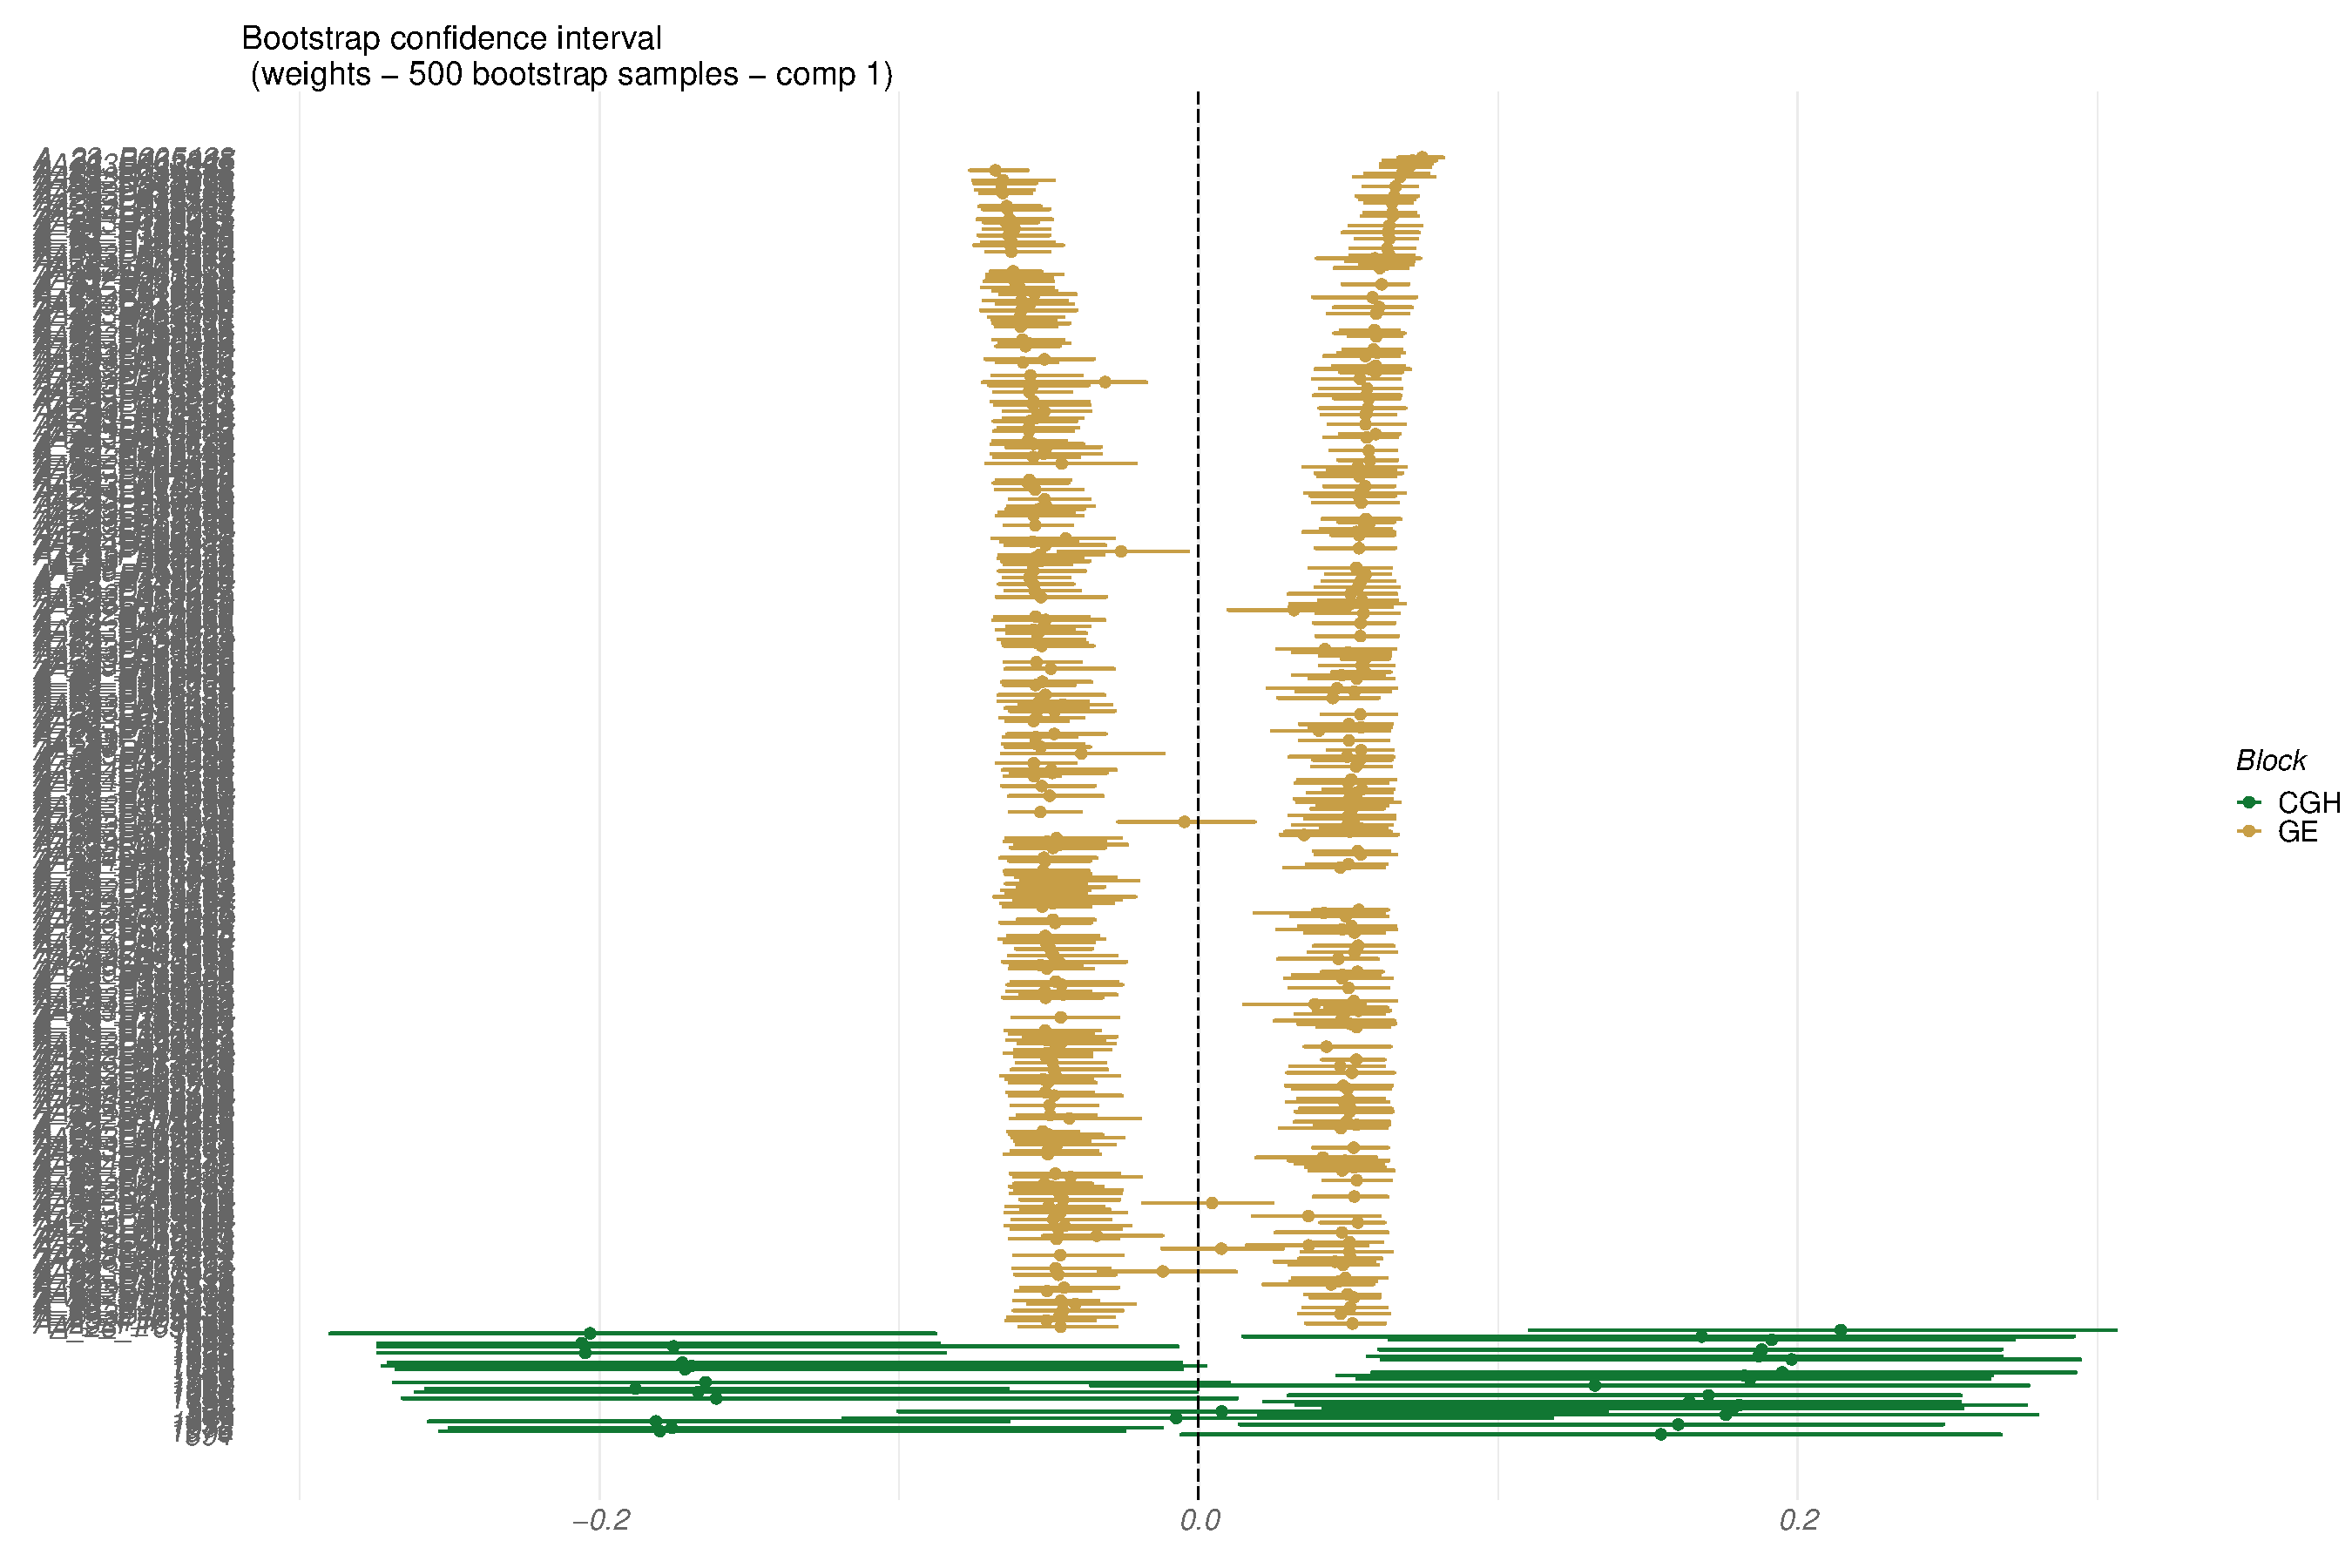
\includegraphics{RGCCA_vignette_files/figure-latex/unnamed-chunk-46-1} \end{center}

\end{CodeChunk}

\normalsize

Of course, it is still possible to determine the optimal sparsity
parameters by permutation. This is made possible by setting the
\texttt{par\_type} argument to \texttt{"sparsity"} (instead of
\texttt{"tau"}) within the \texttt{rgcca\_permutation()} function.

\footnotesize

\begin{CodeChunk}
\begin{CodeInput}
R> set.seed(123456) # -> very sparse model
R> perm_out = rgcca_permutation(blocks, connection = C, response = 3,
+                                 par_type = "sparsity",
+                                 par_value = 
+                                   matrix(c(0.1, 0.25, 1, 
+                                            0.0710, 0.2000, 1,
+                                            0.0552, 0.1571, 1, 
+                                            0.0395, 0.1143, 1,
+                                            0.0237, 0.0714, 1, 
+                                            0.0080, 0.029, 1), 6, 3, 
+                                          byrow = TRUE),
+                                 n_perms = 5, n_cores = 10)
\end{CodeInput}
\end{CodeChunk}

\normalsize

\footnotesize

\begin{CodeChunk}
\begin{CodeInput}
R> plot(perm_out, cex = 1.3)
\end{CodeInput}


\begin{center}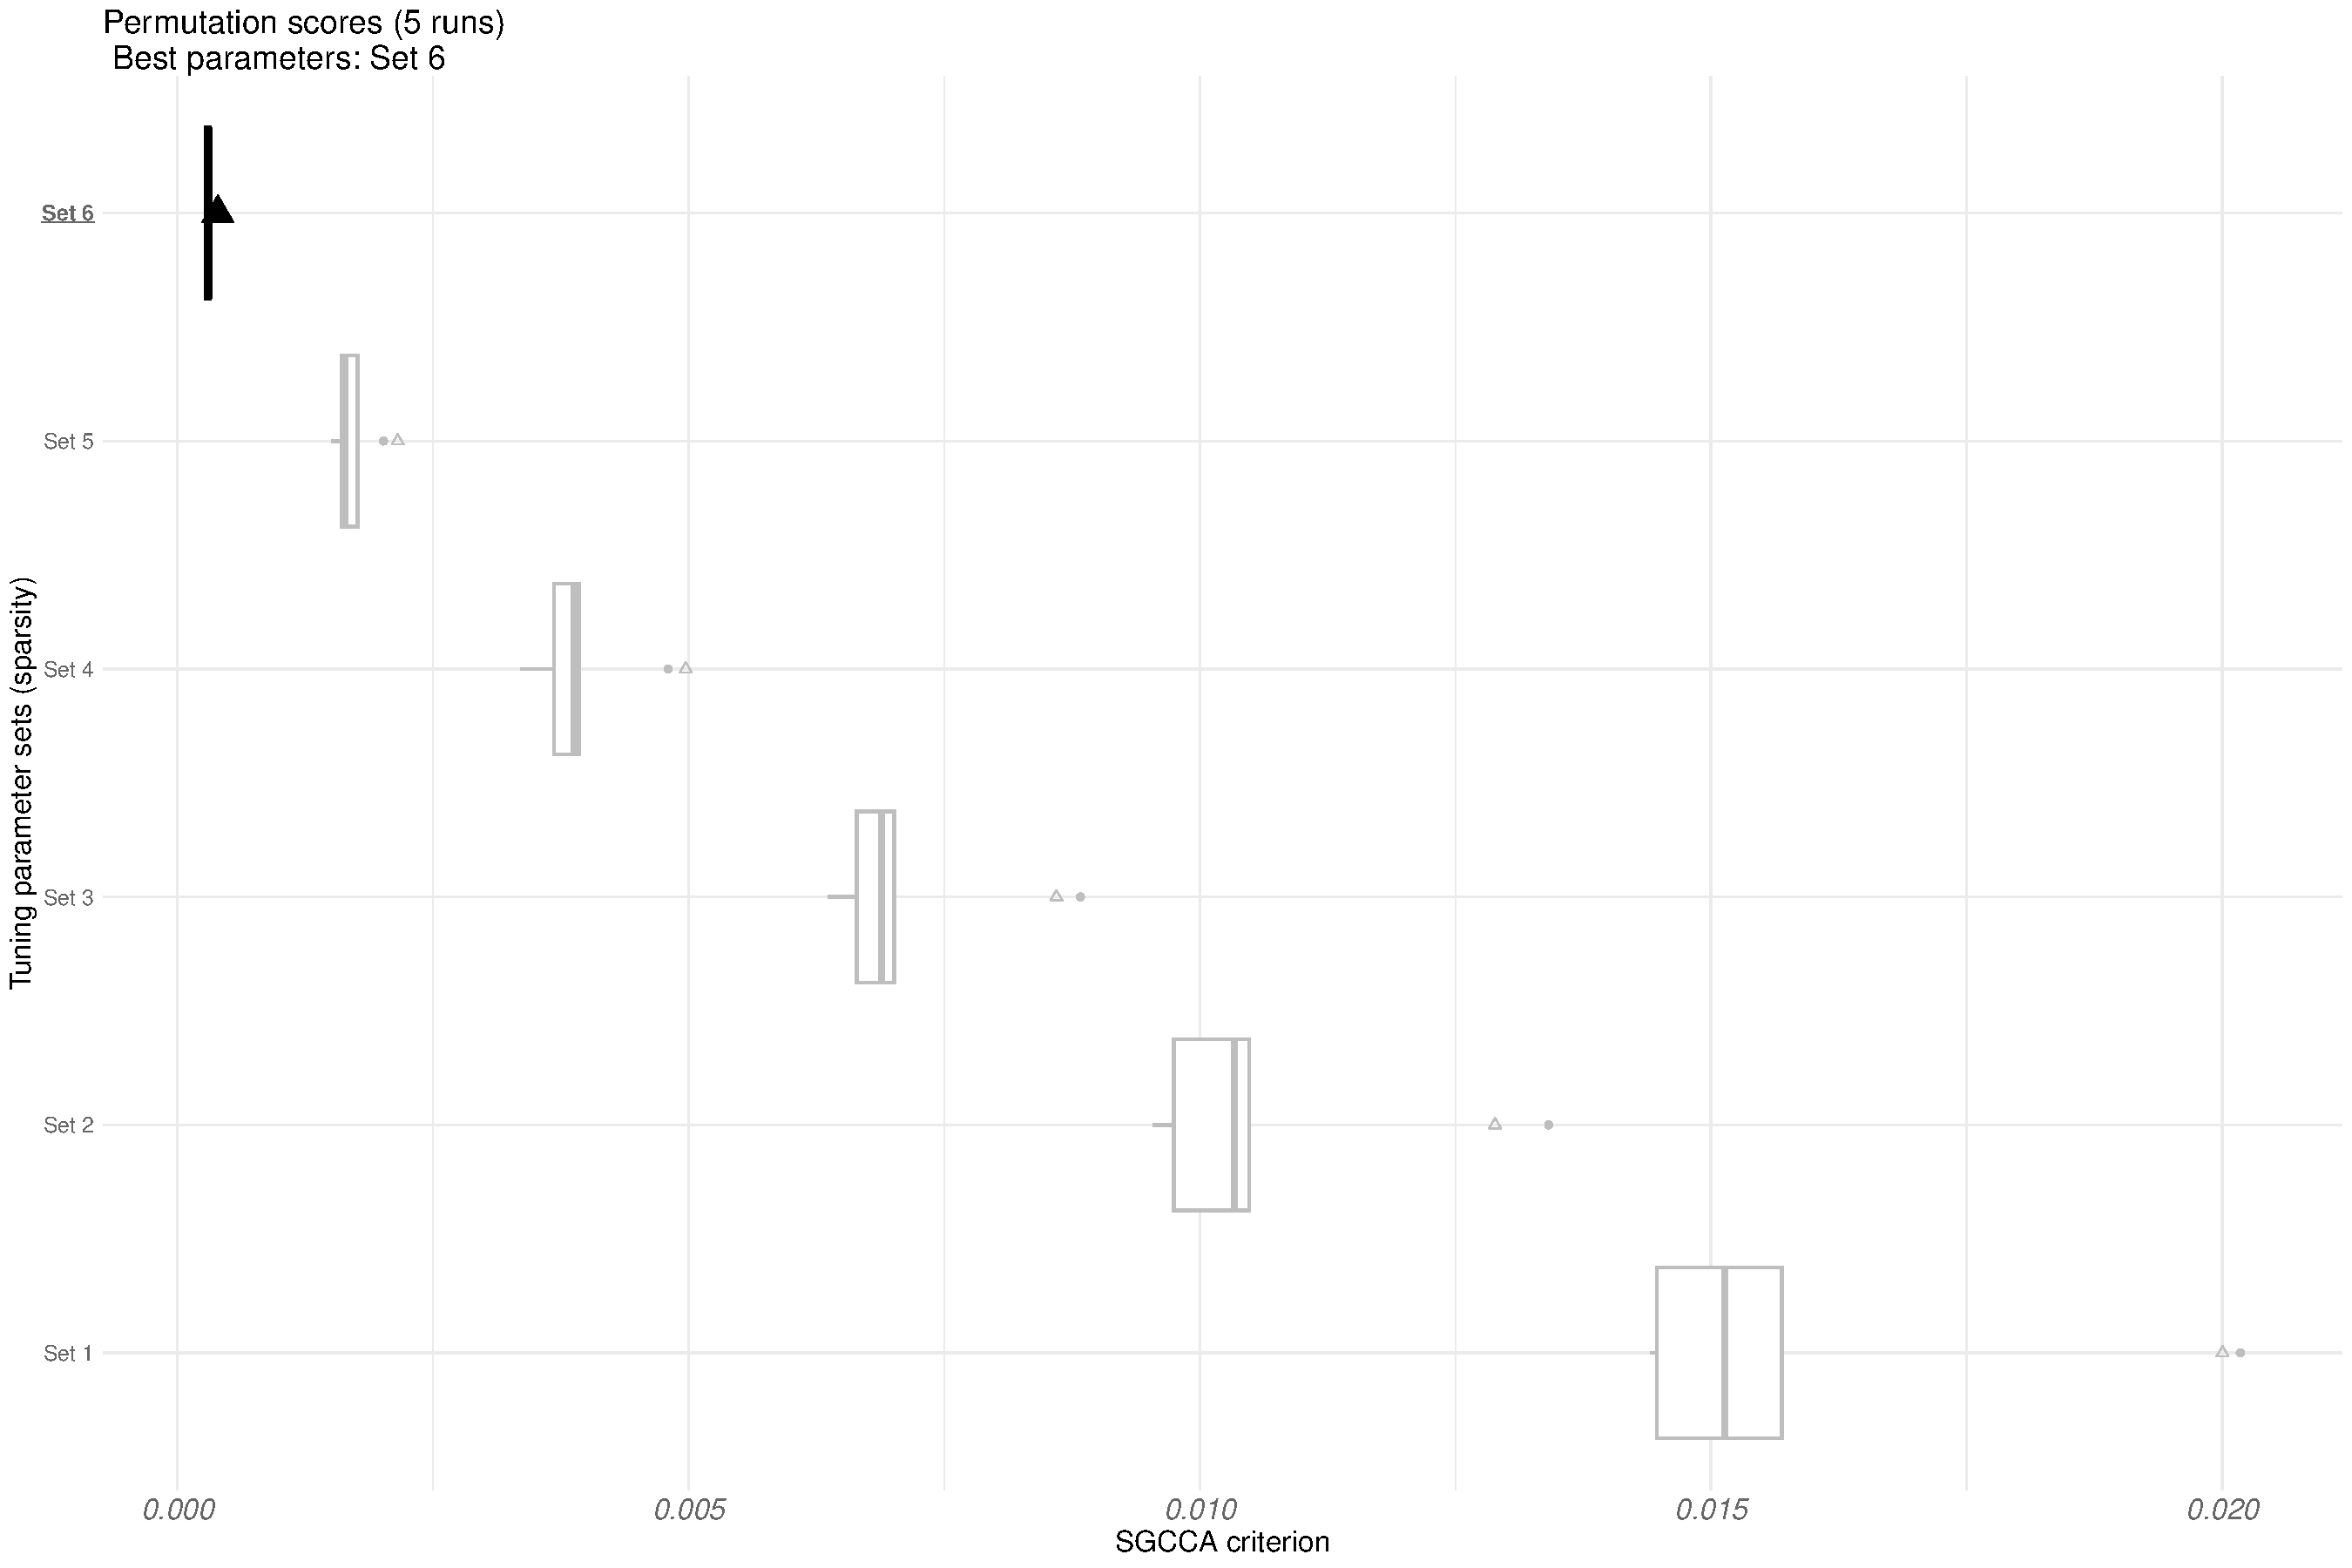
\includegraphics{RGCCA_vignette_files/figure-latex/unnamed-chunk-48-1} \end{center}

\end{CodeChunk}

\normalsize

and then directly used the optimal sparsity parameters as previously:

\footnotesize

\begin{CodeChunk}
\begin{CodeInput}
R> rgcca_opt = rgcca(perm_out)
\end{CodeInput}
\end{CodeChunk}

\normalsize

\footnotesize

\begin{CodeChunk}
\begin{CodeInput}
R> fit_stab = rgcca_stability(rgcca_opt, 
+                            keep = sapply(rgcca_opt$a, 
+                                          function(x) mean(x!=0)),
+                            n_boot = 100, verbose = TRUE, n_cores = 15)
\end{CodeInput}
\begin{CodeOutput}
Bootstrap samples sanity check...OK
\end{CodeOutput}
\end{CodeChunk}

\normalsize

and then apply the bootstrap procedure on the most stable variables.

\footnotesize

\begin{CodeChunk}
\begin{CodeInput}
R> boot_out = rgcca_bootstrap(fit_stab, n_boot = 500)
\end{CodeInput}
\begin{CodeOutput}
All the parameters were imported from the fitted rgcca_stability object.
\end{CodeOutput}
\begin{CodeOutput}
Bootstrap samples sanity check...OK
\end{CodeOutput}
\end{CodeChunk}

\normalsize

The bootstrap results can be visualized using the generic
\texttt{plot()} function.

\footnotesize

\begin{CodeChunk}
\begin{CodeInput}
R> plot(boot_out, block = 1:2, 
+      display_order = FALSE, 
+      n_mark = 2000, cex = 1.3)
\end{CodeInput}


\begin{center}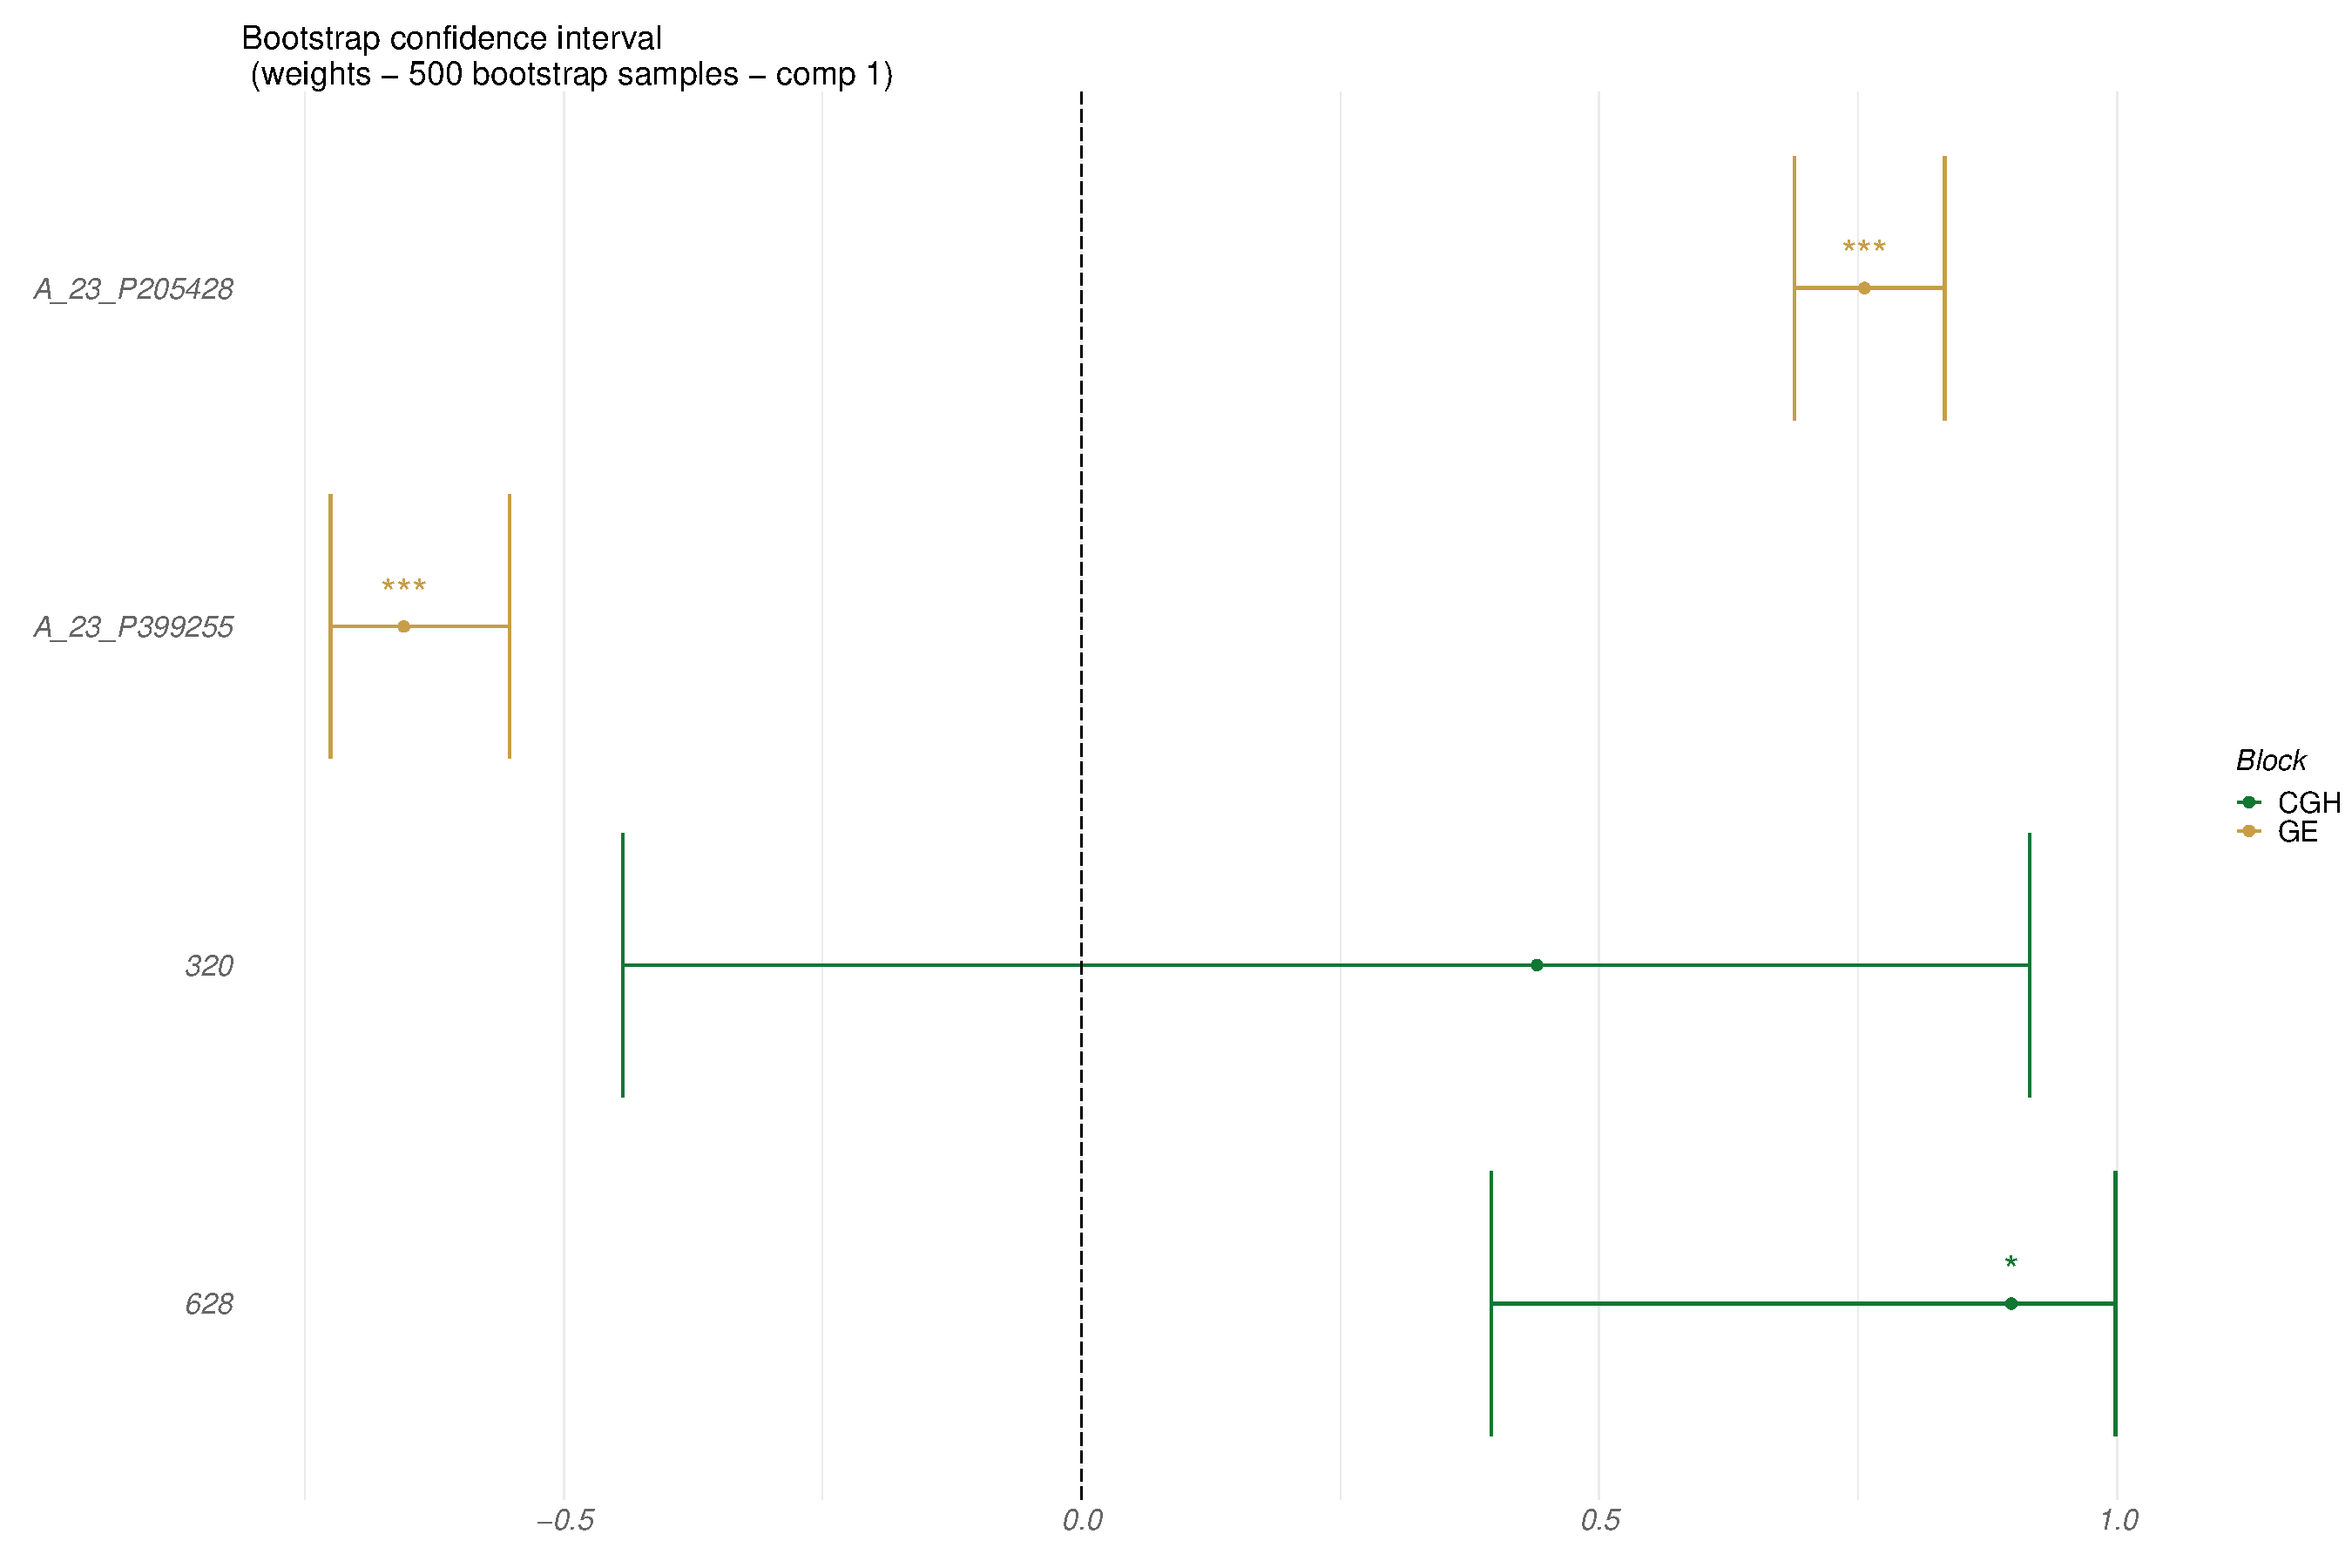
\includegraphics{RGCCA_vignette_files/figure-latex/unnamed-chunk-52-1} \end{center}

\end{CodeChunk}

\normalsize

One component per block has been built (GE1 for \(\mathbf{X}_1\) and
CGH1 \(\mathbf{X}_2\)), and the graphical display of the tumors obtained
by crossing GE1 and CGH1 and labeled according to their location is
shown below.

\footnotesize

\begin{CodeChunk}
\begin{CodeInput}
R> plot(fit_stab, type = "sample", block=1:2, 
+      comp=1, resp = as.character(Loc), 
+      cex = 1.3
+      )
\end{CodeInput}
\begin{figure}

{\centering 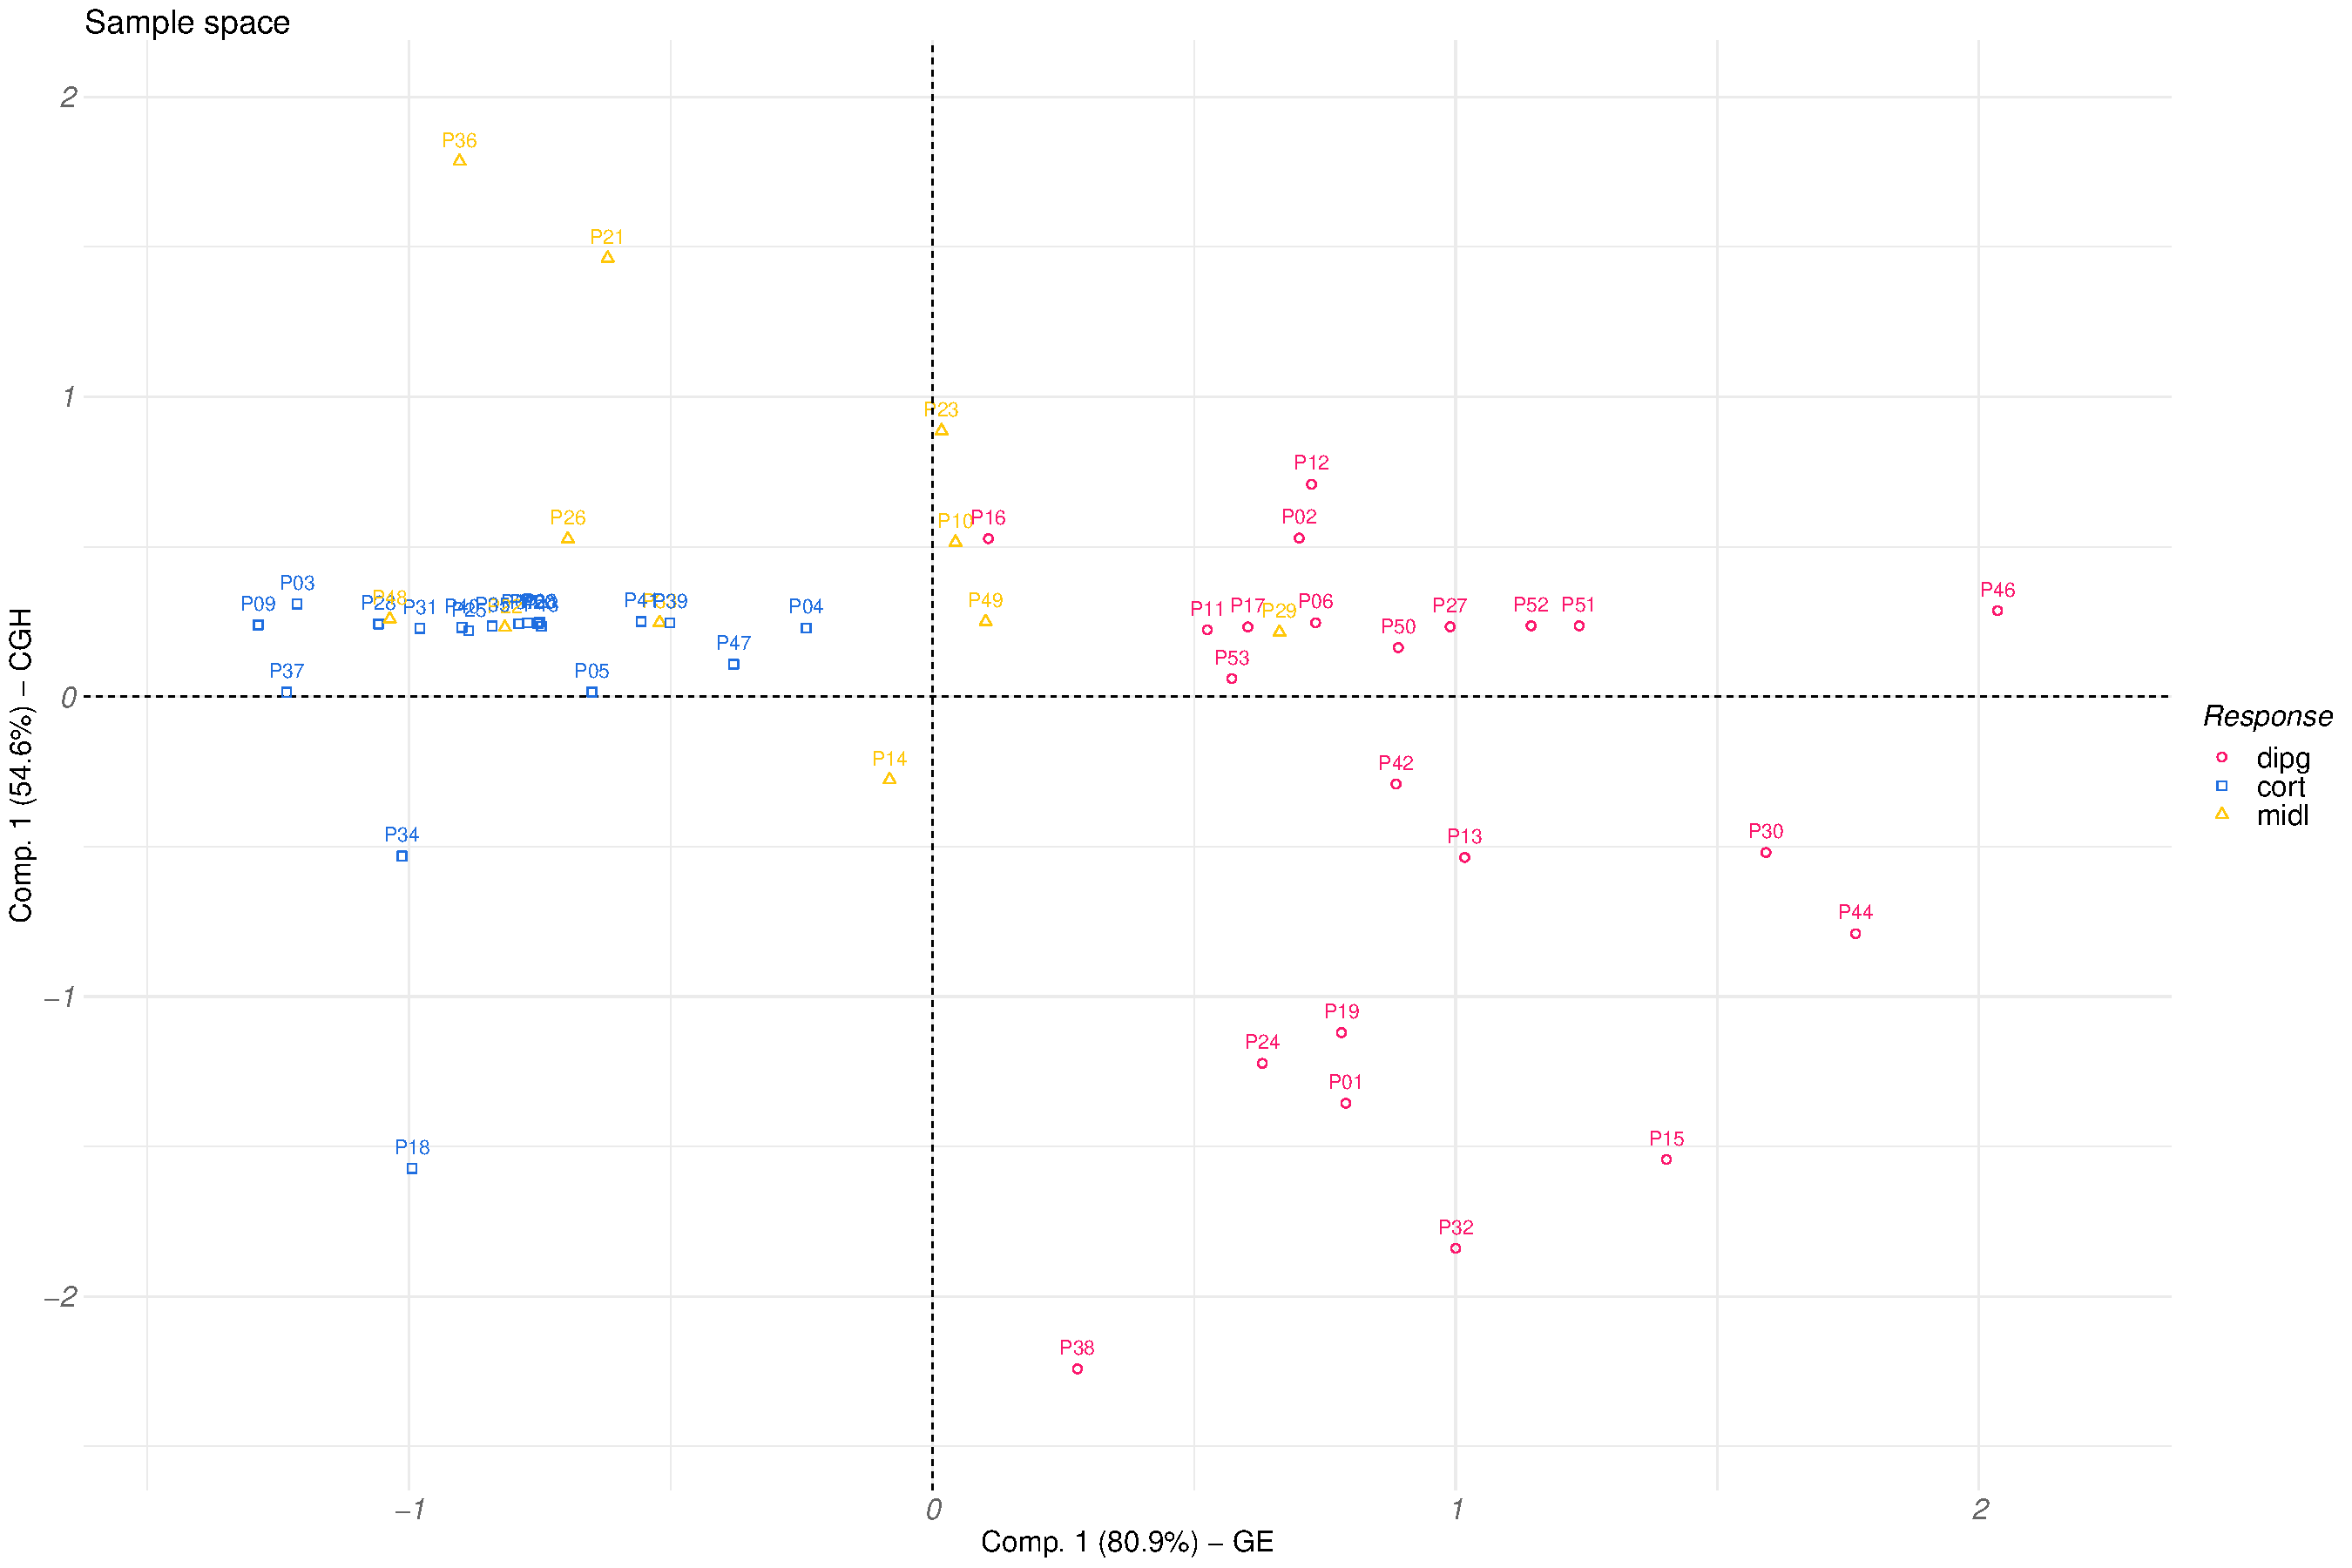
\includegraphics{RGCCA_vignette_files/figure-latex/unnamed-chunk-53-1} 

}

\caption[graphical display of the tumors obtained by crossing GE1 and CGH1 and labeled according to their location]{graphical display of the tumors obtained by crossing GE1 and CGH1 and labeled according to their location.}\label{fig:unnamed-chunk-53}
\end{figure}
\end{CodeChunk}

\normalsize

We observe that \texttt{GE} contains much more discriminative
information than \texttt{CGH}.

\hypertarget{conclusion}{%
\section{Conclusion}\label{conclusion}}

The RGCCA framework gathers sixty years of multiblock component methods
and offers a unified implementation strategy for these methods. The
RGCCA package is available on the Comprehensive R Archive Network (CRAN)
and on github \url{https://github.com/rgcca-factory/RGCCA}. This release
of the RGCCA package includes:

\begin{itemize}
\item Several strategies for determining automatically the shrinkage 
parameters/level of sparsity: Schaffer \& Strimmer's analytical formulae,  
cross-validation or permutation strategy.

\item A bootstrap resampling procedure for assessing the reliability of the 
parameters estimates of S/RGCCA.

\item Dedicated functions for graphical displays of the output of RGCCA 
(sample plot, correlation circle, biplot, ...).

\item Multiblock data faces two types of missing data structure: (i) if an 
observation $i$ has missing values on a whole block j and (ii) if an 
observation i has some missing values on a block j (but not all). For these two 
situations, it is possible to exploit the algorithmic solution proposed for PLS 
path modeling to deal with missing data (see [@Tenenhaus2005], page 171).

\item Special attention has been paid to recover the results of other R packages 
of the literature including `ade4` and `factomineR`.
\end{itemize}

The RGCCA framework is constantly evolving and extended. Indeed, we
propose RGCCA for multigroup data \citep{Tenenhaus2014b} and RGCCA for
multiway data \citep[\citet{Girka2023}]{Gloaguen2020}. In addition,
maximizing successive criteria may be seen as suboptimal from an
optimization point of view where a single global criterion might be
preferred. A global version of RGCCA \citep{Gloaguen2020b} which allows
extracting simultaneously several components per block (no deflation
procedure required) has been proposed. Work in progress includes the
integration of this novel approaches in the next release of the package.

\renewcommand\refname{References}
\bibliography{biblio.bib}



\end{document}
